
\documentclass[12pt]{ociamthesis}  % default square logo
%\documentclass[12pt,beltcrest]{ociamthesis} % use old belt crest logo
%\documentclass[12pt,shieldcrest]{ociamthesis} % use older shield crest logo

%\usepackage[activate={true,nocompatibility},draft,tracking=true,kerning=true,spacing=true,factor=1100,stretch=10,shrink=10]{microtype}
%\DisableLigatures[T]{encoding = *, family = * }
% activate={true,nocompatibility} - activate protrusion and expansion
\usepackage{microtype}
\DisableLigatures[T]{}
\usepackage{setspace}


% final - enable microtype; use "draft" to disable
% tracking=true, kerning=true, spacing=true - activate these techniques
% factor=1100 - add 10% to the protrusion amount (default is 1000)
% stretch=10, shrink=10 - reduce stretchability/shrinkability (default is 20/20)

%%%%%%%%%%%%%%%%%%%%%%%%%% FONTS %%%%%%%%%%%%%%%%%%%%%%%%%
%Palatino
\usepackage[sc]{mathpazo}
\renewcommand{\normalsize}{\fontsize{11pt}{13pt}\selectfont}
\usepackage[light]{kpfonts}

% Latin modern
%\usepackage{lmodern}

%\usepackage[T1]{fontenc}
%\usepackage{kpfonts,baskervald}
% Times
%\usepackage[varg]{txfonts}


% New Century Schoolbook
%\usepackage{fouriernc}

% Minion pro
%\usepackage{MnSymbol}
%\usepackage[mathlf,textlf,minionint]{MinionPro}
% - use below for mix of text and maths numbers
%%\usepackage[mathlf,minionint]{MinionPro}
%\usepackage[T1]{fontenc}
%\usepackage{textcomp}

% Utopia
%\usepackage{fourier}

% bitstream charter
\usepackage[T1]{fontenc}
%\usepackage[latin1]{inputenc}
%\usepackage[bitstream-charter]{mathdesign}
%\usepackage[urw-garamond]{mathdesign}

% Linux libertine
%\usepackage[T1]{fontenc}
%\usepackage{libertine}

%%%%%%%%%%%%%%%%%%%%%%%%%%%%%%%%%%%%%%%%%%%%%%%%%%%%%%%%%

% Line numbers
%\usepackage[displaymath, mathlines]{lineno}
%\linenumbers

%\renewcommand{\sfdefault}{phv}

% Changing section headings
\usepackage{titlesec}
\titleformat{\section}
  {\normalfont\fontsize{14}{16}\bfseries}{\thesection}{1em}{}
\titleformat{\subsection}
  {\normalfont\fontsize{14}{16}\bfseries\itshape}{\thesubsection}{1em}{}
\titleformat{\subsubsection}
  {\normalfont\fontsize{12}{14}\bfseries\itshape}{\thesubsubsection}{1em}{}

% Paragraph indent larger
\setlength{\parindent}{2em}


\usepackage[font=footnotesize,labelfont=sc]{caption}
%\usepackage[libertine,cmintegrals,cmbraces,vvarbb]{newtxmath}
\usepackage{hyperref}
\usepackage{xcolor}

\usepackage{amsmath}

%alphabetical lists
\usepackage{enumerate}

%chemical formulas
\usepackage[version=3]{mhchem}

%appendices in chapters
\usepackage{appendix}

%to surpress page numbers on full page figs
%\usepackage{floatpag}
%\floatpagestyle{empty}

\usepackage{mdwlist}  % allows tightly spaced lists using the * command


% This part makes nicer chapter headings
% uses the fancychap package
\usepackage[Sonny]{fncychap}
\ChNameVar{\Large}
\ChNumVar{\Huge}
\ChTitleVar{\Large}
\ChRuleWidth{0.5pt}
\ChNameUpperCase



% This part uses fancyhdr to make nice headers
\usepackage{fancyhdr}
\newcommand{\changefont}{%
    \fontsize{9}{12}\selectfont}
\pagestyle{fancy}
\fancyhf{}
\renewcommand{\headrulewidth}{0.5pt}
\fancyhead[RE]{\rmfamily \sc \small \nouppercase \leftmark}
\fancyhead[LO]{\rmfamily \sc \small \nouppercase \rightmark}
%\fancyhead[LE]{\thepage}
%\fancyhead[RO]{\thepage}
\cfoot[LE]{\thepage}
\cfoot[RO]{\thepage}
%\fancyhead[RE]{\changefont\color[gray]{0.5}\leftmark}
%\fancyhead[LO]{\changefont\color[gray]{0.5}\rightmark}
%\fancyfoot[RO,LE]{\thepage}

% No headers or footers on empty pages
\usepackage{emptypage}

\fancypagestyle{myplain}
{
  \fancyhf{}
  \renewcommand\headrulewidth{0pt}
  \renewcommand\footrulewidth{0pt}
  \fancyfoot[C]{\thepage}
}

% Define colours for hyperlinks
\definecolor{dark-red}{rgb}{0.4,0.15,0.15}
\definecolor{dark-blue}{rgb}{0.15,0.15,0.4}
\definecolor{medium-blue}{rgb}{0,0,0.5}
\hypersetup{
    %colorlinks, linkcolor={dark-blue},
    %citecolor={dark-red}, urlcolor={medium-blue}
    colorlinks, linkcolor={black},
    citecolor={black}, urlcolor={black}
}

%load any additional packages
\usepackage{amssymb}
\usepackage[authoryear]{natbib}
\setcitestyle{square}
%\bibliographystyle{abbrvnat}
\bibliographystyle{agufull08}
%input macros (i.e. write your own macros file called mymacros.tex
%and uncomment the next line)
%\nclude{mymacros}



\title{INVESTIGATING MULTI-DECADAL ATMOSPHERE \& OCEAN VARIABILITY}    %your thesis title,
                   %note \\[1ex] is a line break in the title

\author{Jordan L. Thomas}             %your name
\college{Department of Earth and Planetary Science}  %your college
%\renewcommand{\submittedtext}{Draft compiled on:}
\degree{Doctor of Philosophy}     %the degree
\degreedate{February 2018}         %the degree date

%end the preamble and start the document
\begin{document}
\begin{romanpages}          % start roman page numbering

% less strict wrapping
\sloppy

%this baselineskip gives sufficient line spacing for an examiner to easily
%markup the thesis with comments
%\baselineskip=22pt plus1pt % originally 18pt - WS

%set the number of sectioning levels that get number and appear in the contents
\setcounter{secnumdepth}{3}
\setcounter{tocdepth}{3}


\maketitle                  % create a title page from the preamble info
%\nclude{dedication}        % include a dedication.tex file
\begin{abstract}

Natural variability of the atmosphere and ocean are important processes to understand and quantify in order to accurately detect and predict anthropogenic climate change. In order to investigate and quantify natural variability, multiple global climate models (GCMs) are utilized along with observational data. These methods are used to investigate the multi-decadal natural variability of three processes:

First, the natural variability of the Southern Annular Mode (SAM) and Southern Hemisphere westerly jet strength and position are quantified using 14 different GCMs. The magnitude of the natural variability of these quantities is compared with recent observational trends that have been attributed to ozone depletion. While in the literature these three quantities are assumed to have similar variability, the results in this thesis show there are distinct differences between them. In addition, comparison of the modeled natural variability with the observed trends suggest that the observed trends in these three metrics are not decisively outside of the natural variability.

Next, the relationship between oceanic heat and carbon content is examined in a suite of coupled climate model simulations that use different parameterization settings for mesoscale mixing. The different parameterizations result in different multi-decadal variability, especially in the Weddell Sea where the characteristics of deep convection are changed. While there are differences in the variability, there is a robust anti-correlation between global heat and carbon content in all simulations. Global carbon content variability is primarily driven by Southern Ocean carbon variability. This contrasts with global heat content variability, which is primarily driven by variability in the southern mid-latitudes and tropics.

Finally, we explore the relationship between age and oxygen and find that in both observations and a model, the assumed negative linear relationship between age and oxygen is not found both within and directly below the ventilated thermocline at the end of Line W. While observations along Line W shows a decoupling of the biologically-driven age-oxygen relationship, our model analysis indicates that this phenomenon is relatively localized to Line W due to the combination of relatively weak horizontal gradients in age and oxygen resulting reduced along-isopycnal variability and vertical heave acting on a depth offset between age and oxygen extrema.
\par
  \vspace{.5in}
  \textbf{Faculty Advisor and First Reader:} Professor Darryn Waugh \\
  Earth and Planetary Science Department, Johns Hopkins University \\
  \textbf{Second Reader:} Professor Anand Gnanadesikan \\
  Earth and Planetary Science Department, Johns Hopkins University



\end{abstract}

%%% Local Variables:
%%% mode: latex
%%% TeX-master: "thesis"
%%% End:
          % include the abstract
\begin{acknowledgements}
\addcontentsline{toc}{chapter}{Acknowledgements}

Many people have contributed to the creation of this thesis. I would first like
to thank my advisor, Darryn Waugh, for his patience, guidance, and thoughtful
support. I am also deeply indebted to Anand Gnanadesikan, my secondary advisor,
for sharing his knowledge with me throughout this 5 year process. This work would
not be possible without the generous funding from the National Science Foundation
under Grant FESD-1338814. \\

Completing a thesis is a daunting task - one that was made less so with the
support of my husband, Andrew, along with all my closest friends and family.\\

My time in the Earth and Planetary Sciences department has been incredibly enjoyable.
Many thanks to everyone who was a part of it.

\end{acknowledgements}




%%% Local Variables:
%%% mode: latex
%%% TeX-master: "thesis"
%%% End:
   % include an acknowledgements.tex file


\baselineskip=14pt plus4pt % as HA
%\doublespacing

\tableofcontents            % generate and include a table of contents
\listoftables              % generate and include a list of tables
\listoffigures              % generate and include a list of figures

%\chapter*{List of acronyms and abbreviations}
\addcontentsline{toc}{chapter}{List of acronyms and abbreviations}

\begin{description*}

\item[CFC] Chlorofluorocarbon
%\item[CMCC] Centro Euro-Mediterraneo per I Cambiamenti Climatici
\item[CMIP5] Coupled Model Intercomparison Project Phase 5
%\item[DJF] December to February (inclusive)
\item[ENSO] El Ni\~no Southern Oscillation
\item[ERA] Combination of ERA-40 reanalysis (1958--1978) and ERA-Interim (1979--2010)
\item[ESM] Earth System Model
\item[GCM] General circulation model
\item[GFDL] Geophysical Fluid Dynamics Laboratory
%item[IPSL] Institut Pierre-Simon Laplace
%\item[MIROC]
\item[MMM] Multi-model mean
%\item[MPI] Max Planck Institute
%\item[MRI] Meteorological Reseach Institute
\item[piControl] Pre-industrial Control
\item[SAM] Southern annular mode
\item[SH] Southern Hemisphere
\item[SST] Sea Surface Temperature


\end{description*}



%%% Local Variables:
%%% mode: latex
%%% TeX-master: "thesis"
%%% End:


\end{romanpages}             % end roman page numbering
%\baselineskip=22pt plus1pt % originally 18pt - WS
%\baselineskip=22pt plus4pt % as HA
\baselineskip=24pt

% Paragraph spacing
%\usepackage{parskip}
\setlength{\parskip}{6pt}


%now include the files of latex for each of the chapters etc
\graphicspath{{figures/chapter-intro/}} % Specifies the directory where pictures are stored


\chapter{Introduction}
\label{cha:intro}


Anthropogenic climate change has been a hot topic amongst scientists and the public for the past decade. A few of the primary questions associated with climate change relate to how scientists know that climate change is caused by humans and where and when the effects of climate change will be seen. Both of these questions require an understanding about what causes the climate to change over time. Earth's climate is a complex dynamic system and has changed constantly throughout Earth's history. Being able to separate the climate's natural fluctuations from the change caused by anthropogenic activity is essential to being able to accurately predict and detect future changes in climate.

\section{Natural Variability}

One of the primary challenges of assessing the impact of anthropogenic influence on Earth's climate is a lack of understanding of the natural fluctuations of the climate system. Internal climate variability is simply how Earth's climate varies in time without any external forcing. External forcing can be natural in source, including volcanic eruptions, and solar forcing, or anthropogenic, including human emissions of greenhouse gases and human caused land use changes. The term natural variability on the other hand is typically used to refer to fluctuations in Earth's climate caused solely by natural forcing (internal or external), and not including anthropogenic influence.

Natural variations in the climate system, also referred to as 'climatic noise', (Madden, 1976; Schneider and Kinter, 1994; Wunsch, 1999; Feldstein, 2000) are a result of non-linear dynamical and biological processes in the atmosphere and ocean operating on a variety of spatial and temporal scales. The most common example of natural variability is the El Ni\~no-Southern Oscillation (ENSO), which is a result from the non-linear interactions between the atmosphere and ocean in the Equatorial Pacific. While ENSO is perhaps the most famous of all the atmospheric climatic modes of variability, there are multiple modes of variability in the atmosphere and ocean which interact with each other.

A further complicating matter is that climate variations happen on all timescales: paleo-climatic, centennial, multi-decadal, decadal, inter-annual, and seasonal, in addition to on all spatial scales from regional to global. Global variability on long timescales is generally the best understood, however regional variability is generally the most important when it comes to understanding and interpreting recent trends in observational data.

Quantification of natural variability is important to climate science for many reasons. First, natural variability is key to determine climate predictability. Climate predictability was first defined in 1975 (Academy of sciences publication, 1975) as a measure of signal-to-noise, where the signal is any potentially predictable long-term (> 1 year) climate feature, and the noise is natural variability. Having an estimate of natural variability allows us to answer the question - how large does a trend need to be in order to detect it? Without an idea of what the natural variability of a given feature is, it is nearly impossible to determine if a signal lies within the noise of the climate system.
Another reason quantifying natural variability is important relates to projection uncertainty. Characterizing uncertainty for climate change projections is important for purposes of detection and attribution and for strategic approaches to adaptation and mitigation (Deser et al, 2012). Uncertainty in future climate change comes from three main sources: forcing, climate model response, and internal variability (Lovenduski et al 2015, Hawkins and Sutton 2009; Tebaldi and Knutti 2007).

A final example of where understanding natural variability is important is in the evaluation of global climate models. Because of observational limitations and the inability to experiment on the entire earth system, climate models are developed and used to further our knowledge of the planet and climate system. Climate models are typically validated against the mean state of a given climate feature. For example, to assess the accuracy of the ocean module in a climate model, one might compare the average sea surface temperature (SST) in a pre-industrial control model run to the average of many years of SST observations from similar period (via proxy records). While this method is useful for assessing the mean state of the climate model, it does not give any information about the variability of the model. The model could have vastly larger variance than the observations, which would not be captured by comparing the means.
One of the largest challenges with estimating natural variability is a lack of observational estimates. In an ideal situation, scientists would be able to quantify natural variability using observations of the Earth system. However, because natural variability operates on all time and spatial scales, this would require millions of observations across the entire globe. Global natural variability over thousands of years is estimated using proxy records of Earth's climates; however, regional variability on shorter timescales (decadal to multi-decadal) is much more of a challenge to quantify because it requires finer resolution of observations.

To supplement the limited observational estimates of natural variability, scientists often turn to global climate models to quantify natural variability. Unlike observational records, global climate models have a consistent spatial and temporal resolution. Global climate models can also be used to simulate multiple realizations of Earth's climate over thousands of years, to generate a statistical distribution of climate variability in absence of external forcing. Because no single climate model is a perfect representation of Earth's dynamical and biological processes, multiple models are often employed to reduce the uncertainty due to model configuration. This method of quantifying natural variability also comes with challenges. Primarily, global climate models are very computationally expensive and require extensive resources and time to generate a simulation. Additionally, to best quantify natural variability, multiple simulations without any anthropogenic forcing should be performed. Because of the emphasis on simulating future change, fewer resources have traditionally been put toward conducting non-anthropognically forced simulations.

In this thesis, natural variability in both physical fields (winds and temperature) and biogeochemically active fields (carbon and oxygen) is examined across multiple scales.


\section{Thesis Overview}
This thesis takes an investigative look at the multi-decadal natural variability of three important components of the climate system: the Southern Hemisphere westerly jet, oceanic carbon and heat content, and North Atlantic oxygen and age. These three components of the atmosphere and ocean variability were selected because of the important role they have in the response of the global climate system.

\subsection{Chapter 2 - Southern Hemisphere Westerly Jet}
The Southern Hemisphere (SH) westerly jet is incredibly important for driving the Southern Ocean circulation, which has strong influence on global climate. The strong, eastward flowing winds of the drive subsurface Ekman transport towards the north. This northward flowing water is colder than the water it encounters (and therefore denser) and subsequently sinks into the interior to form Antarctic Intermediate Water - a process known as ventilation. Closer to the Antarctic continent, overlaying easterly winds drive the surface water towards the south where waters interact with the Antarctic sea ice and dense water is formed (formation of Antarctic Bottom Water). The resulting divergence of water at the surface of the Southern Ocean allows for deep water (primarily North Atlantic Deep Water) to rise to the surface and interact with the atmosphere (Figure 2).

This process of water rising to the surface, interacting with the atmosphere, and subsequently sinking back into the interior allows for increased atmosphere-ocean gas exchange and results in the Southern Ocean being very influential on global climate. the Southern Ocean is one of the most important oceans for regulating global climate. Recent estimates suggest that the Southern Ocean is responsible for 75\% of the heat uptake and 30\% of the carbon uptake (Frolicher et al 2014)

Recent studies suggest that anthropogenic ozone depletion and greenhouse gas induced warming has already had an impact on the SH westerly jet through a strengthening and shift towards the Antarctic continent. In this Chapter 2, we utilize 14 state-of-the-art global climate models from modeling centers around the world to quantify the natural variability in the SH westerly jet. We then compare the model-estimated natural variability to the recently observed trends in the jet strengthening and pole-ward shift. Our results suggest that a combination of natural variability and anthropogenic forcing are required to explain the observed trends in the SH westerly jet.

\subsection{Chapter 3 - Oceanic Heat and Carbon Variability}
Chapter 3 turns to the role of natural variability in the Southern Ocean on the global and regional oceanic heat and carbon budget. One particular phenomenon that holds significant implications for global climate is deep ocean convection. The high-latitude Southern Ocean is weakly stratified with cold fresh water overlaying slightly warmer saliter water of nearly identical density (Martinson, D. G., 1991). Deep convection in this region occurs when this weakly stratified surface layer is perturbed and becomes denser than the under-laying waters resulting in the entire water column turning over. This results in the surface waters being subducted deep into the ocean, and old deep water being brought up to the surface.

While only one of these deep convective events have been observed in the real Earth's Southern Ocean (the Weddell Polynya which persisted through the winters of 1974-1976) many global climate models have consistent periodic convection events in this region (deLavergne et al.). Because of the intense exchange of surface and deep waters associated with deep convection, these events have been shown to have profound impacts on global climate (Gordon, A. L 1982, Cabre et al).

In Chapter 3, we use multiple simulations from a coarse-resolution climate model to explore the temporal variability of oceanic carbon and heat and investigate how this global heat and carbon variability is impacted by Southern Ocean deep convective events. We show that the Southern Ocean deep convection has significant influence on the magnitude of global oceanic heat and carbon variability, however the relationship between oceanic heat and carbon remains consistent with varying convection.

\subsection{Chapter 4 - Age and Oxygen Relationship}
Chapter 4 builds on this idea that biological and physical responses to changes in circulation may differ. Oceanic age refers to the time since the ocean water was last in contact with the atmosphere. This derived tracer is used to estimate the rate of ocean ventilation and overturning circulation. Oxygen is another tracer that is important to understanding ocean circulation and biological activity. Age and oxygen are generally thought to have a strong negative correlation because biological utilization reduces oxygen concentrations in the ocean interior where the age is the oldest. This presumed relationship is often times used in ocean biogeochemistry and oceanography to estimate changes in biological activity and ocean circulation.

We focus on an observational data set in the North Atlantic and look at how changes in oxygen and oxygen utilization relate to changes in ventilation age. We show that in the observational record and in a global climate model simulation, along Line W in the North Atlantic this expected relationship between age and oxygen is more complicated due to the different spatial structure of sources of apparent oxygen utilization and age in the deep ocean.


\begin{figure}
\centering
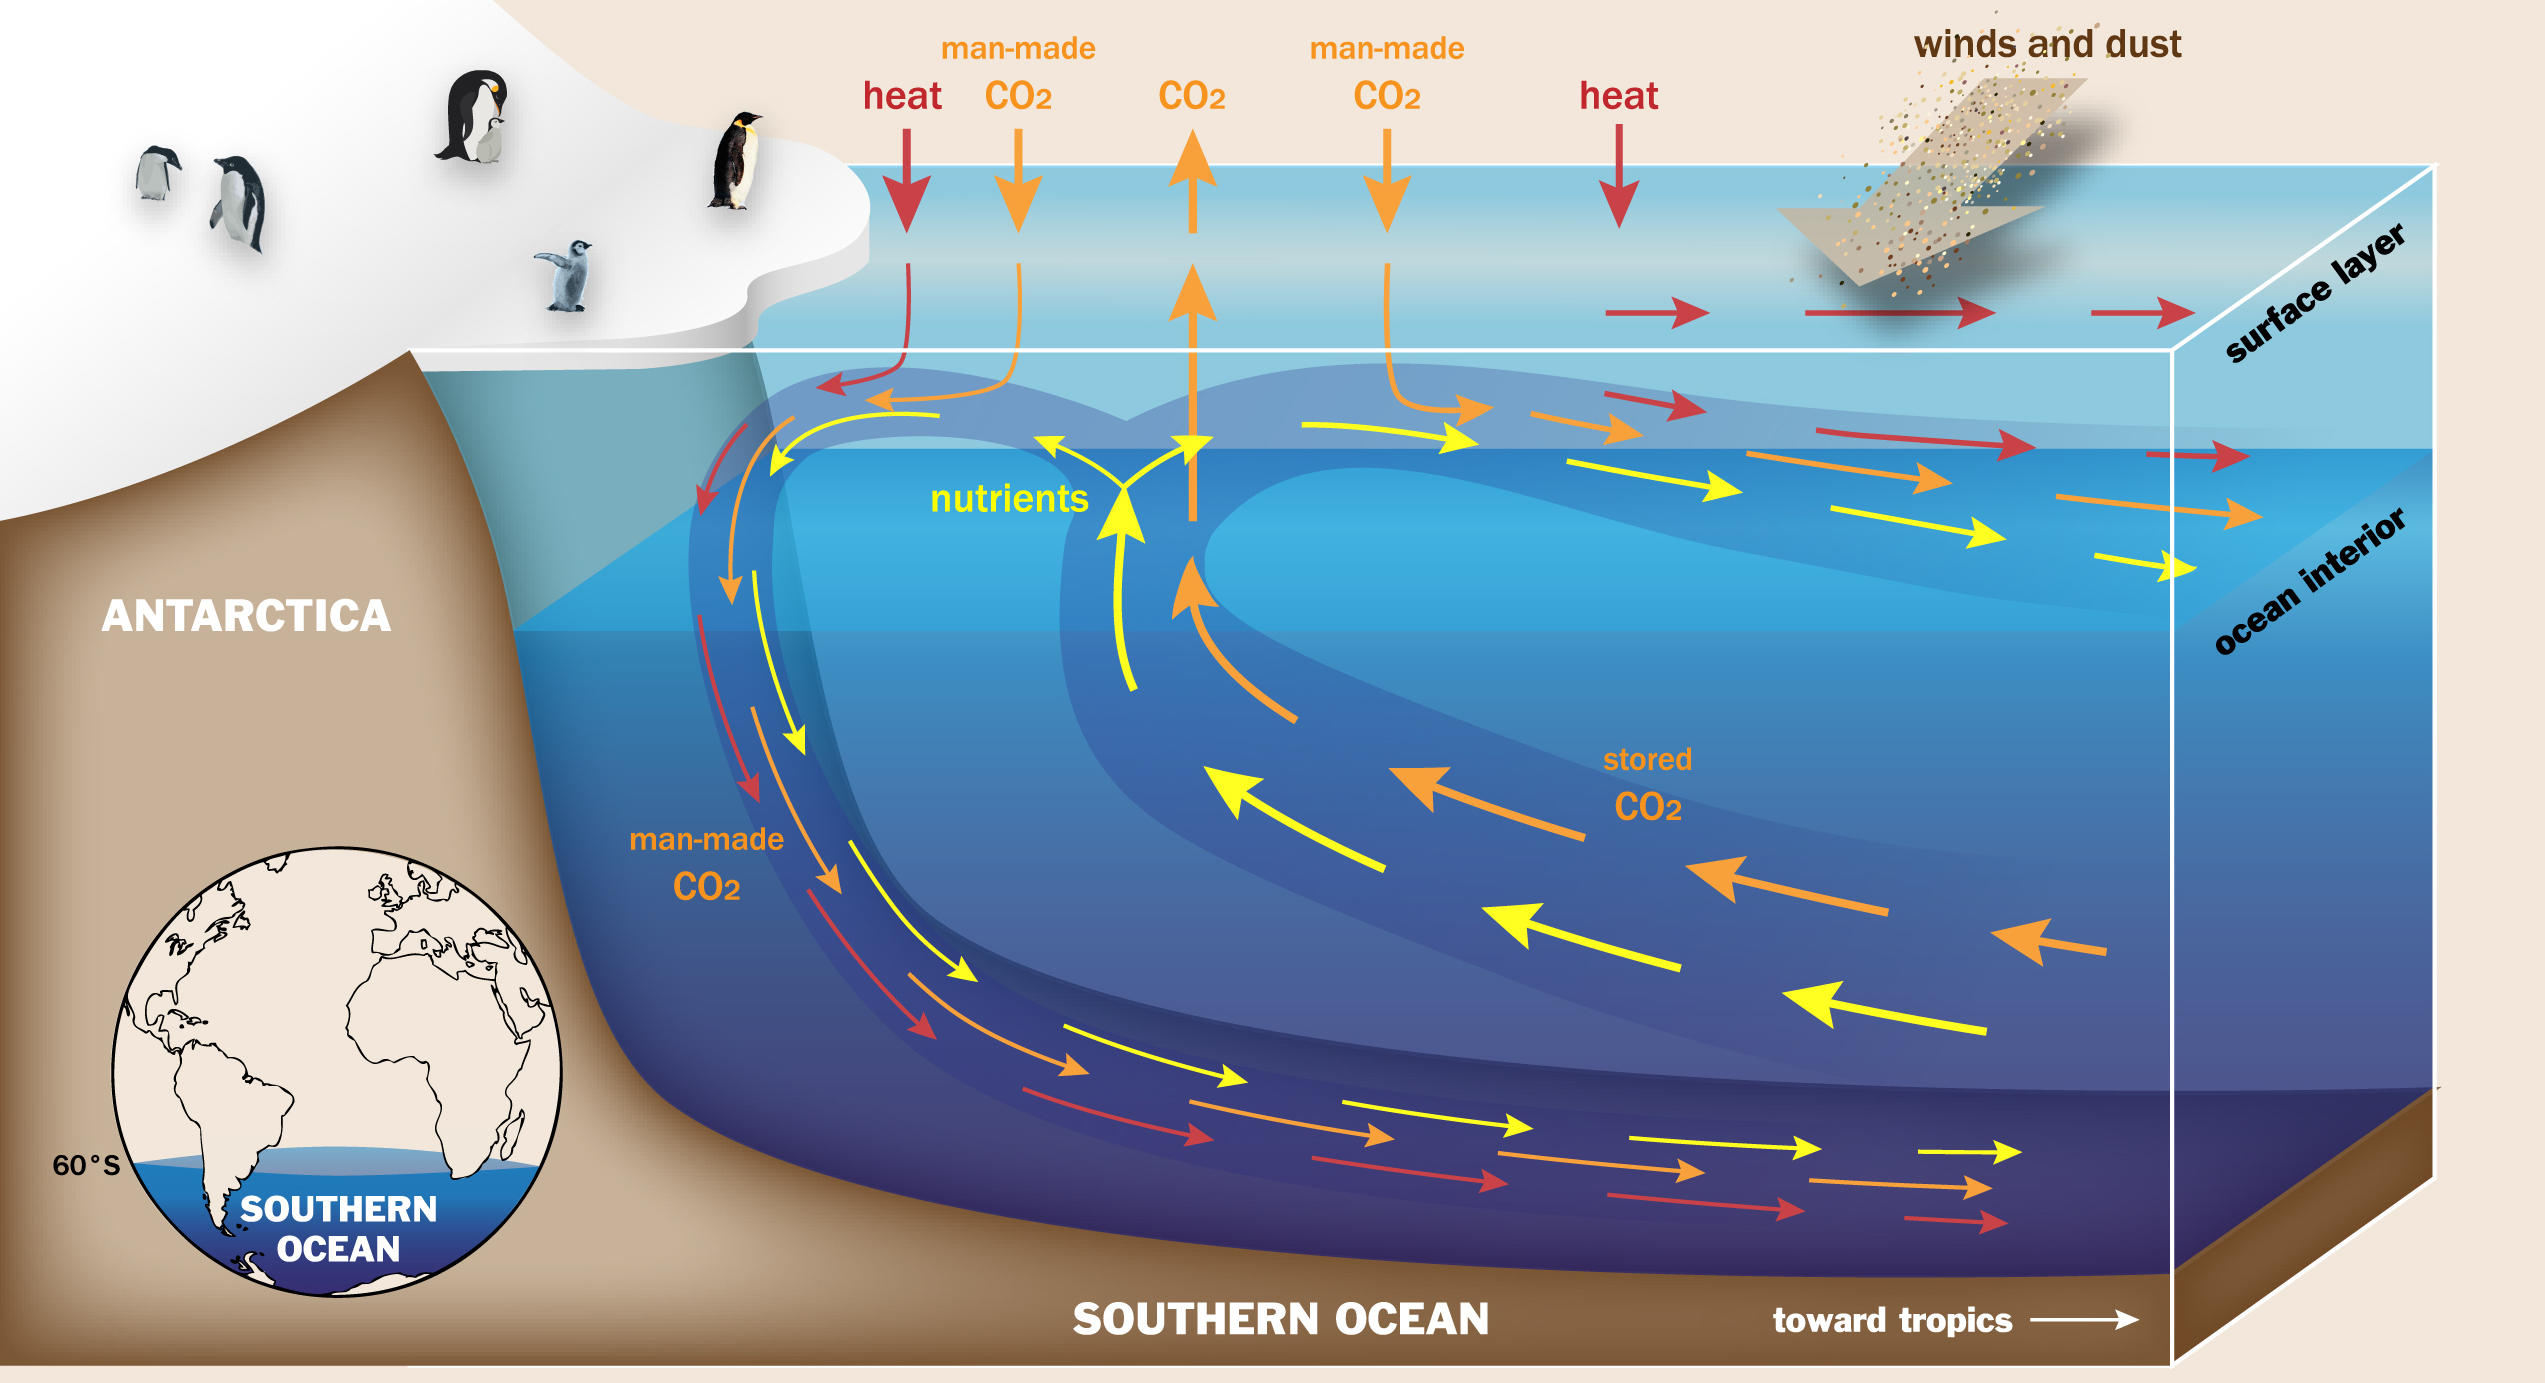
\includegraphics[width=33pc]{Southern_Ocean.jpg}
\caption{Schematic depicting Southern Ocean circulation. Figure by Ilissa Ocko, courtesy of Princeton University.}
\label{fig:carbon_cycle}
\end{figure}


%%% Local Variables:
%%% mode: latex
%%% TeX-master: "thesis"
%%% End:

\chapter{Recent trends and natural variability}
\label{cha:SHcirc}

\begin{quotation}
  Much of the work contained in this chapter is based upon \citet{Thomas2015},
  published in \emph{Geophysical Research Letters}.
\end{quotation}

\section{Overview and aims}

The Southern Ocean plays a critical role in the ocean overturning circulation
and moderating global climate through carbon and heat uptake
\citep{Khatiwala2009,Gnanadesikan1999}, with approximately 40$\%$ of
anthropogenic carbon and 75$\%$ of heat entering the ocean south of 30$^\circ$S
\citep{Frolicher2015,Sabine2004}. The leading mode of Southern Hemisphere
(SH) extratropical variability, the Southern Annular Mode (SAM), has been shown
to directly affect this overturning circulation and the distribution of
anthropogenic carbon uptake by altering the magnitude and location of the
westerly jet \citep{Hall2002b,Mignone2006b,SenGupta2006e}.  It is
therefore important to understand the variability in the SH extratropical
circulation.

Observations and reanalyses have shown a positive trend in SAM and jet magnitude
over the last couple decades along with a poleward shift in the jet location
\citep{Thompson2000b,Thompson2002e} in addition to trends in subtropical sea
surface temperature, Antarctic sea ice extent, ocean ventilation and gyre
circulation \citep{Parkinson2012c,Swart2012a,Waugh2013b,Roemmich2007b}.
Additionally, studies have detected anthropogenic influences in surface pressure
and the westerly jet \citep{Gillett2003,Gillett2005}. These trends in the
SAM and consequently the jet have been largely attributed to ozone depletion in
the SH stratosphere during austral summer \citep{Previdi2014f,Gillett2013,
Gillett2003a}. However, there is also evidence that this positive phase trend
in the SAM is due in part to greenhouse gas warming \citep{Arblaster2006,
Lee2013f,Gillett2013}.

While there is evidence of anthropogenic forcing, understanding the forcing in
the context of natural variability is difficult given the lack of in-situ
observations and satellite information prior to 1979. Previous studies have
tried to quantify the natural variability in the SH using proxy records
\citep{MARSHALL2003,Visbeck2009} and climate models \citep{Latif2013}.
Understanding the relative contribution of natural variability and anthropogenic
forcing to recent trends is critical to understanding how global climate will be
influenced in the future.

In this study, we aim to further estimate the natural variability of the SH
extratropical circulation by using the Coupled Model Intercomparison Project
Phase 5 (CMIP5) pre-industrial control model runs. We examine five metrics of
the SH extratropical circulation: the SAM, the jet location defined using the
850mb winds ($U_{lat}$) and the surface wind-stress ($\tau_{lat}$), the jet
magnitude defined by the 850mb winds ($U_{max}$) and the surface wind-stress
($\tau_{max}$). We turn to CMIP5 pre-industrial model runs to quantify the
natural variability of these five metrics to address the following questions:
Can recently observed trends in SH circulation occur in CMIP5 piControl model
runs due to natural variability alone, do the CMIP5 models historical
(1980-2004) runs show significant trends in the circulation metrics, and do
these simulated historical trends capture the characteristics of the observed
trends?

\section{Methods}


In order to examine the natural multi-decadal-scale variability in the SH
circulation we use a combination of pre-industrial control (``piControl'') and
historical (1980 to 2004) runs from models. Table 1 lists the models used in
this study, the length of their piControl run and the number of historical runs.
The models were chosen based on the availability of monthly-mean fields of sea
level pressure, 850mb zonal winds and zonal wind-stress for both piControl and
historical runs.  We focused on the austral summer (averaged over December,
January and February) because this is the season where the largest trends are
observed \citep{Thompson2002e,Thompson2011}.

From the monthly sea-level pressure, we calculated the SAM as the zonal sea
level pressure difference between $65^{\rm o}$ and $40^{\rm o}$ degrees South.
For the sake of comparisons across different models, we chose to leave the SAM
as a surface pressure difference as opposed to normalizing by the standard
deviation as done in \citet{Gong1999} to avoid normalizing by different
standard deviations across models. Additionally, we examine the SH  westerly
jet magnitude and location calculated using both zonal surface wind-stress
($\tau_{max}$ and $\tau_{lat}$) and 850mb zonal winds ($U_{max}$ and $U_{lat}$).
To find the jet maximum and location, the maximum zonal-mean wind-stress/850mb
winds and the surrounding 4 grid-points were isolated and interpolated to a
0.1-degree meridional grid. A quadratic polynomial was then fit to the
interpolated data and the maximum magnitude and location was found.

%%% Table
{\small
\begin{table}[t]
\caption{CMIP 5 models used in this study.}
\centering
\begin{tabular}{ l p{5cm} p{5cm} }
\hline
 Model & piControl model run length (years) & Historical model ensemble  runs \\
\hline
 CanESM2 & 996 & 1\\
 %\hline
 CNRM CM5 & 850 & 10\\
 %\hline
 GFDL ESM2M & 500 & 1\\
 %\hline
 IPSL CM5a LR & 1000 & 6\\
 %\hline
 IPSL CM5a MR & 300 & 3\\
 %\hline
 IPSL CM5b LR & 300 & 1\\
 %\hline
 MIROC ESM & 531 & 3\\
 %\hline
 MIROC ESM CHEM & 255 & 1\\
 %\hline
 MIROC5 & 200 & 5\\
 %\hline
 MPI ESM LR & 1000 & 3\\
 %\hline
 MPI ESM MR & 1000 & 3\\
 %\hline
 MRI CGCM3 & 500 & 3\\
 %\hline
 NOR ESM1m M & 501 & 1\\
 %\hline
 NOR ESM1m ME & 252 & 1\\
\hline
\end{tabular}
\end{table}
}
%%% End Table

While there are no trends (i.e., drift) in these metrics over the length of the
piControl time-series (order 250-1000 years), strong multi-decadal trends are
found. Time-series in SAM from a high-varying model (MPI ESM MR) and a
low-varying model (MIROC5) are shown in Figure~\ref{fig:ch2_fig1}a and c
respectively. As highlighted in red, there are multiple 25-year periods that
have strong trends even though there is no trend over the entire time-series.
In order to quantify the variability of these multi-decadal-scale trends, we
calculate the linear trend of each metric (SAM, $\tau_{max}$, $\tau_{lat}$,
$U_{max}$, and $U_{lat}$) for consecutive and overlapping 25-yr trends for each
model's piControl run (\citet{Polvani2013e} performed a similar analysis for
sea ice extent in piControl runs).

\begin{figure}[t]
\noindent
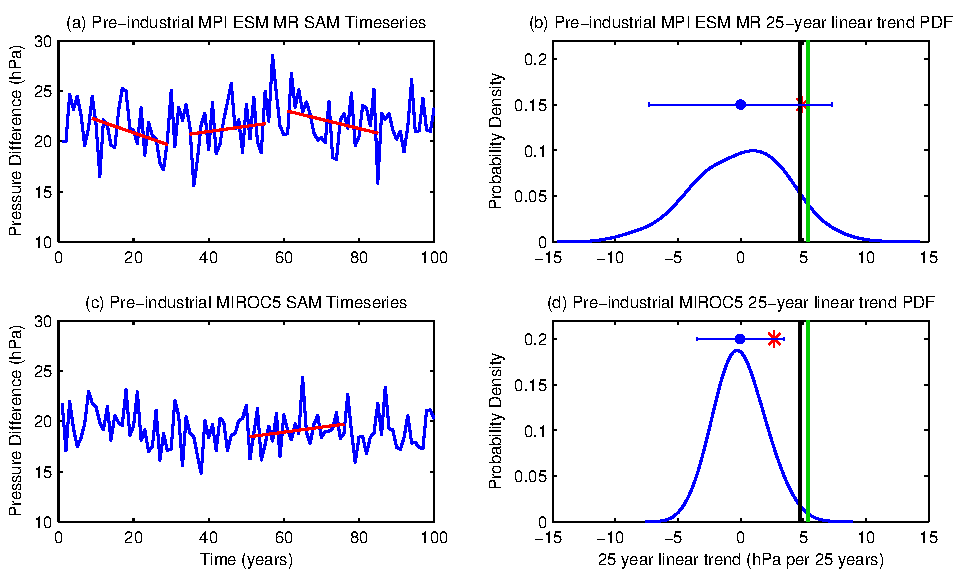
\includegraphics[width=\linewidth]{figures/chapter-SHcirc/2014jgrl-p01.pdf}
\caption{SAM time-series for (a) MPI ESM MR and (c) MIROC5 piControl runs over
the first 100 years. The red lines indicate periods where the trend is greater
than the average reanalysis trend between 1980-2004. Figures b and d show the
probability density functions for the 25-year linear SAM trends in MPI ESM MR
and MIROC5  respectively. The blue dot represents the mean of the 25-year trends
while the whiskers extend 2 standard deviations. The vertical lines represent
the observed trends: NCEP R1 (green), NCEP R2, ERA-Int, and JRA-55 (black), and
the red asterisk shows the magnitude of the historical model run trend (first
ensemble member). }
\label{fig:ch2_fig1}
\end{figure}

We focus on the period 1980-2004 because reanalyses are unreliable before the
implementation of satellites in 1979 (\citet{Swart2012a} Figure 1). Our
analysis goes up until 2004 in order to compare with the CMIP5 historical model
runs, which are typically run until year 2005. To verify that period length does
not influence our results, the same analysis with CMIP5 piControl model runs and
observations for the 34-year period between 1980-2014 was conducted (not shown).
The results are essentially identical to those reported below as the observed
changes over this period are either the same size or smaller than over the
1980-2005 period and the modeled trends are only slightly smaller.

The distribution of these 25-yr trends for the model piControl run is a measure
of the natural multi-decadal variability in each model (in other words, the
model internal variability with no anthropogenic influences). As an example,
the probability density function (PDF) of these 25-year linear trends for the
MPI ESM MR and MIROC5 models are shown in Figure 1b and d. The blue curve shows
the probability density of the 25-year linear trends for the SAM, and  the
whisker plot shows the mean (blue circle) and 2 standard deviations (whisker
extent) of the 25-year trends.  The means of the 25-year trends (blue dot) are
near zero, consistent with there being no drift in the piControl runs, but the
trend for any individual 25-year period varies from -10 to +10 hPa per 25 yrs
(with standard deviation of around 4 hPa per 25 yrs). Throughout the rest of the
paper we shall use the whiskers to represent the distribution of 25-year trends
from the model piControl runs. Each CMIP5 model has a different piControl run
length, which could potentially impact our model-model comparisons. However,
subsampling the output from 1000 year piControl runs shows limited sensitivity
of the standard deviation of 25-yr trends for run lengths between 250 and 1000
yrs.

To compare the observations with the modeled natural variability, we used four
reanalysis products: NCEP Reanalysis 1 (NCEP-1) \citep{Kalnay1996}, NCEP
Reanalysis 2 (NCEP-2) \citep{Kanamitsu2010}, ERA-Interim \citep{Dee2011},
and JRA-55 \citep{KOBAYASHIa} during the period 1980-2004. We also
calculated the linear trend between the years 1980-2004 from the model
historical runs, and compared both with the observed trends and model natural
decadal variability.  The vertical lines in Figure 1b and d represent the
1980-2004 reanalysis trends and the red asterisk shows historical simulation
trend.

\section{Results \& Discussion}

\subsection{Natural Variability}

We first examine the distribution of 25-year linear trends from CMIP5 piControl
runs. Figure 2 shows, as whisker plots, the distributions of 25-year linear
trends of (a) SAM, (b) $U_{lat}$, (c) $\tau_{lat}$, (d) $U_{max}$, and (e)
$\tau_{max}$, for each model . For all five metrics, the mean 25-year linear
trend (blue circles) is around zero for all the models, as expected for unforced
model runs with no drift. The width of the whiskers is, however, variable across
the different models, indicating differences in the multi-decadal variability
among the models. Models with larger whiskers are more variable with stronger
multi-decadal trends than models with smaller whiskers.

The variability of the whisker width among the models differs among the five
metrics. The SAM (Figure 2a) shows the most variability among the models, with
the width of the whiskers ranging from 3 hPa per 25 years to 10 hPa per 25 years
(the mean and 2 sigma of the whisker length for the ensemble of models is $6 \pm
3$ hPa per 25 years). This indicates there is little agreement in the magnitude
of the natural variability of the unforced system in SAM among the CMIP5 models.
The jet location variability, $U_{lat}$ (Figure 2b) and $\tau_{lat}$ (Figure 2c)
also differs across the various models,  but the differences are not as
pronounced as in the SAM (whisker width is $2 \pm 0.75$ degrees per 25 years).
There is even less variability between the models in  jet magnitude. For the
850mb winds (Figure 2d) the whisker extent is $0.75 \pm 0.25$ $m s^{-1}$ per 25
years, while for magnitude of the surface wind-stress (Figure 2e) it is
approximately $0.015 \pm 0.005$ Pa per 25 years.

{\small
\begin{table}
\caption{Probability of obtaining averaged reanalysis trend by only natural variability (first three columns) and natural variability + historical multi-model ensemble trend (second three columns). }
\centering
\begin{tabular}{p{4cm}cccccc}
\hline
  & \multicolumn{3}{c}{\footnotesize{Natural Variability}} & \multicolumn{3}{c}{\footnotesize{Nat. Variability + Hist. Ensemble}} \\
\cline{2-4}
\cline{5-7}

 Model  & $SAM$ &  $U_{loc}$ & $U_{max}$ & SAM & $U_{loc}$ &  $U_{max}$\\
\hline
 CanESM2   & \textbf{5.98}\% & 0.09\% & 0.03\% & \textbf{35.4}\% & \textbf{9.77}\% & 1.77 \%\\
  %\hline
 CNRM CM5 & 4.18 \% & 0.21\% & 0.28\% & \textbf{34.2}\% & \textbf{6.45}\% & \textbf{6.71} \%\\
 %\hline
  GFDL ESM2M & \textbf{5.41}\% & 1.05\% & 0.71\% & \textbf{32.1}\% & \textbf{7.32}\% & \textbf{6.92} \%\\
  %\hline
 IPSL CM5a LR & \textbf{17.24}\% & 2.79\% & 0.31\% & \textbf{39.5}\% & \textbf{13.0}\% & \textbf{5.54}\%\\
 %\hline
 IPSL CM5a MR & \textbf{9.29}\% & 1.84 \% & 0.30\% & \textbf{33.0}\% & \textbf{7.31}\% & 4.70\%\\
 %\hline
 IPSL CM5b LR & \textbf{16.3}\% & 3.70 \% & 1.49\% & \textbf{39.8} \% & \textbf{15.3}\% & \textbf{9.56}\%\\
 %\hline
 MIROC ESM & \textbf{5.69}\% & 0.078\% & 0.032\% & \textbf{37.8}\% & 3.80\% & 2.36 \%\\
 %\hline
 MIROC ESM CHEM & \textbf{10.24}\% & 0.52\% & 0.044\% & \textbf{34.4}\% & \textbf{7.27}\% & 1.78\%\\
 %\hline
 MIROC5 & 1.18\% & 0.005\% & 0.36\% & \textbf{26.7}\% & 2.13\% & 3.65 \%\\
 %\hline
 MPI ESM LR & \textbf{8.40}\% & 1.70\% & 0.81\% &  \textbf{34.8} \% & \textbf{10.4}\% & \textbf{6.67}\%\\
 %\hline
 MPI ESM MR & \textbf{9.50}\% & 1.81\% & 0.71\% & \textbf{40.3}\% & \textbf{12.3}\% & \textbf{7.61}\%\\
 %\hline
 MRI CGCM3 & \textbf{5.14}\% & 0.27\% & 0.93\% & \textbf{37.0}\% & \textbf{7.24}\% & \textbf{9.33}\%\\
 %\hline
 NOR ESM1m M & 3.98 \% & 0.09 \% & 0.05\% & \textbf{32.6}\% & \textbf{5.30}\% & 1.70 \%\\
 %\hline
 NOR ESM1m ME & 3.63\% & 0.09\% & 0.04\% & \textbf{33.3}\% & 4.46\% & 2.98 \%\\
\hline
\multicolumn{3}{l}{\footnotesize{*Bolded values indicate a probability of 5\% or higher.}}
\end{tabular}
\end{table}
}

To better understand how these metrics compare to each other, we compare the
linear correlations of each of the jet metrics with the SAM (Figure 3). The
highest correlations occur between the SAM and the jet latitude metrics, with
average $R^2$ values of 0.7 for both $\tau_{lat}$ and $U_{lat}$. The
correlations between the SAM and jet magnitude metrics are significantly lower
with average $R^2$ values at 0.5, with the $R^2$ values for correlations of SAM
with $\tau_{max}$ always being greater than that of SAM with $U_{max}$.

The comparison of magnitude of natural decadal variability of the different
metrics and correlation between the metrics shows our first key result: The SAM,
jet location and jet magnitude metrics are not interchangable.

\subsection{Observed trends}

With a description of the natural variability from the piControl run for each
model, we now compare the observed reanalysis trends to the modeled natural
variability to examine if the observed trend is forced or natural. In each panel
in Figure~\ref{fig:ch2_fig2}, the dashed horizontal lines show the magnitude of the observed
reanalysis trends.  As expected from the above analysis there are differences
among the different metrics.

\begin{figure}
\noindent
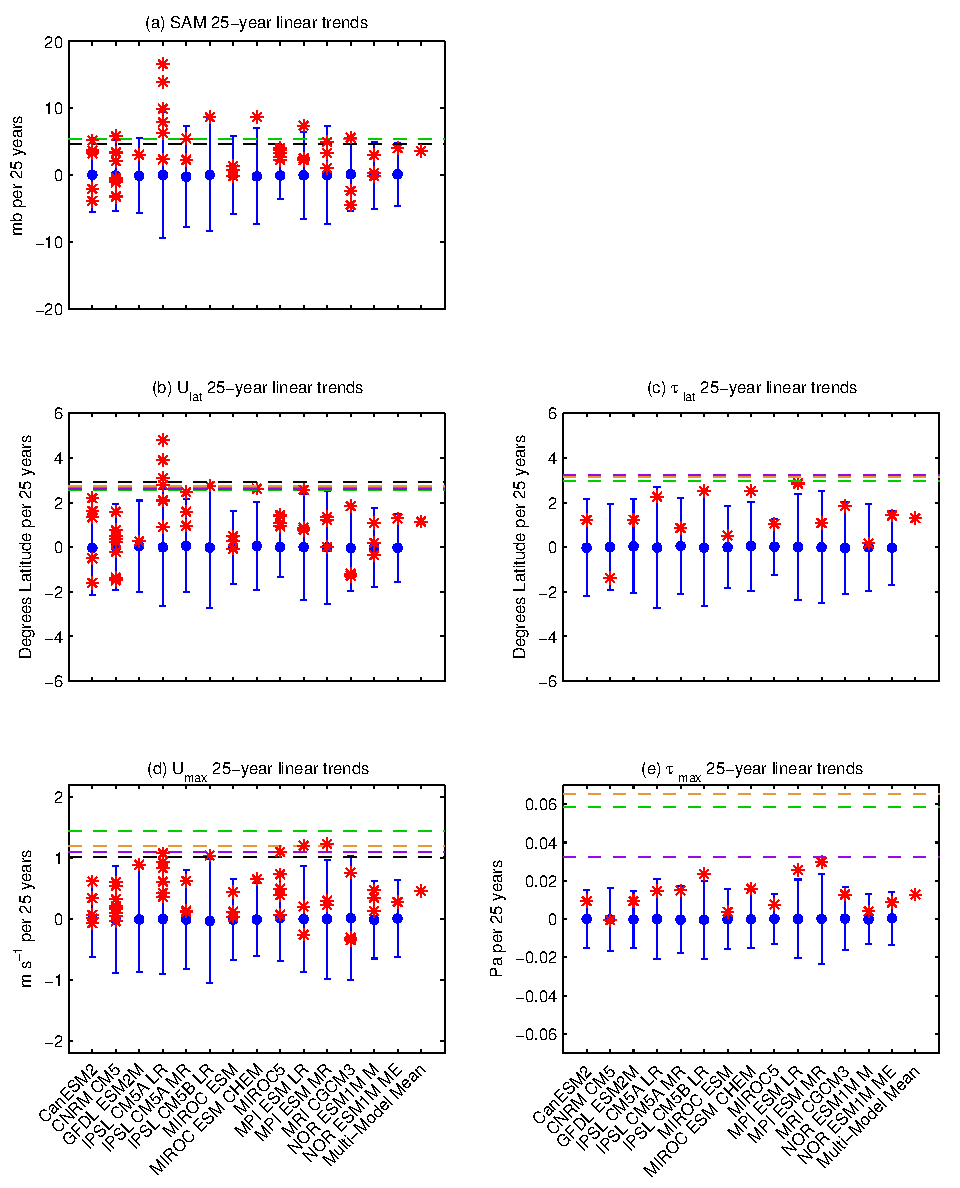
\includegraphics[width=1\linewidth]{figures/chapter-SHcirc/2014jgrl-p02.pdf}
\caption{Natural variability, historical trends and observations for (a) SAM,
(b) 850mb jet latitude, (c) wind-stress jet latitude, (d) 850mb jet magnitude,
and (e) wind-stress jet magnitude. Blue circles show the mean of the piControl
25-year linear trends indicating model drift. Whisker length is 2 standard
deviations. Red points show the historical run trends for each ensemble member.
Horizontal dashed lines indicate the absolute value of the observed trends: NCEP
R1 (green), NCEP R2 (orange), ERA-Int (purple), and JRA-55 (black).}
\label{fig:ch2_fig2}
\end{figure}

The observed SAM trend observations lie just within the whiskers for most of the
models, indicating the observed trends lie within the model natural variability.
To quantify this further, the probability of each model randomly obtaining a
trend with the magnitude of the average reanalysis SAM trend or larger is shown
in table 2 (column 1). 10 of the 14 models have a probability of 5\% or greater,
and thus there is a significant (at the 5\% level) probability of  obtaining the
observed 25-year trend in the piControl simulations by chance alone. In other
words, the observed trend over the period 1980-2004 in the SAM lies just within
the edge of natural variability as described by these models. This result also
holds for the period 1980-2014 (not shown).

The observed $\tau_{lat}$ and $U_{lat}$ trends are just outside the model's
natural decadal variability (Figure 2b and c).  If we calculate the probability
of each model obtaining the observed average reanalysis $U_{lat}$ trend (table
2, column 2), then we see that no models have a probability of 5\% or greater;
however, 6 of the 14 have greater than a 1\% probability. Thus, there is not a
significant (at the 5\% level) probability of obtaining the observed trend using
natural variability alone.

In contrast, the observed trends in $\tau_{max}$ and $U_{max}$ are both outside
the natural variability as described by the models (Figure 2d and e). The
probability of obtaining the average reanalysis $U_{max}$ trend in all but one
of the piControl models is less than 1\% (table 2, column 3) and therefore there
is not a significant (at the 1\% level) probability of the natural variability
reproducing the observed trend. The probabilities of the piControl $\tau_{max}$
and $\tau_{lat}$ obtaining the observed trends are not shown in table 2, but are
consistent with the $U_{max}$ and $U_{lat}$ probabilities.

The above shows that the observed trends in the SAM largely lie at the edge of
natural multi-decadal variability of the piControl model runs. However, this
does not necessarily mean that the observed trends are not forced by
anthropogenic activities, merely that the observations can contain a large
component of natural variability in the SAM. The observed trend in the jet
location and magnitude, however, is outside the variability of most models
piControl runs. This does suggest an external force driving the jet to
strengthen and shift over this 25-year period.

\subsection{Model historical trends}

We now examine the model historical runs to understand how the modeled trends
compare to the modeled natural variability and to compare the modeled trends
with the observed trends. The red asterisks in Figure 2 represent the 25-year
trend for each historical run (the number of historical runs varies among the
models).

There is considerable variability amongst the models in the magnitude of the
trends, but for all five metrics the vast majority of the simulated historical
trends are of the same sign (increase in SAM, poleward shift and strengthening
of the jet). This consistency in sign indicates that external (anthropogenic)
forcing is causing at least part of the trend.  However,  the magnitude of the
historical trends are almost all within the natural multi-decadal variability of
the corresponding model (i.e. within the whiskers). Thus while the response in
the models between 1980 and 2004 is due (at least in part) to forcing, the
response does not overwhelm the natural variability.

For the SAM, the magnitude of the individual historical ensemble member trends
are largely within the estimated natural variability and highly variable, with
some ensemble members having trends of the opposite sign to the observations
(dashed horizontal lines). Because the observed trends are generally within the
natural decadal variability of the models a close agreement between individual
historical ensemble members and observed trends would not be expected due to the
high component of natural variability. Most of the ensemble members have
positive trends and the magnitude of the multi-model ensemble mean historical
trend is similar to the observations. This further suggests an anthropogenic
forcing pushing the SAM towards positive phase.

The same comparison for jet location and magnitude yields different results.
The observed trends in the jet metrics are outside the natural variability of
the models, and generally larger than the modeled historical trends (especially
for the magnitude of the wind stress). A possible cause for this is that the
observed trends are due to anthropogenic forcing that is not well represented
(or under represented) in the models.  However, another possibility is that
there are issues with the reanalyses and the reanalyses are overestimating the
real trend.  This may especially be the case for the NCEP reanalyses, where the
wind stress trends  are significantly outside the model natural variability but
the 850 hPa winds are just outside the model natural variability.

If we consider the observed trends to be a combination of natural variability
and external forcing, and if we use the ensemble-mean historical trend as a
representation of the forced response, we can better capture the observed trend.
The last 3 columns in table 2 show the probability of obtaining the mean
reanalysis trend from a combination of each model's natural variability and the
multi-model ensemble mean historical trend (results for $\tau_{lat}$ and
$\tau_{max}$ are not shown, but are consistent with $U_{lat}$ and $U_{max}$).
The probabilities for each metric are substantially greater, indicating that
there is a significant probability, in most models, that the observed trends are
due to this combination of natural variability and anthropogenic forcing. This
does not exclude the possibility that the models are systematically biased low,
or that the reanalyses are biased high, but it suggests that the mismatch is
smaller than might be suggested from previous work \citep{Swart2012a}.

\begin{figure}
\noindent
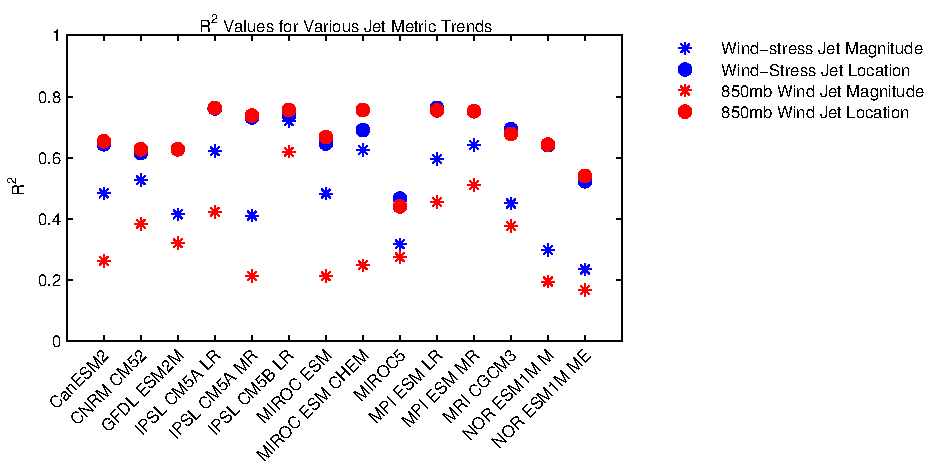
\includegraphics[width=0.9\linewidth]{figures/chapter-SHcirc/2014jgrl-p03.pdf}
\label{fig:ch2_fig3}
\caption{Correlation coefficient squared for correlation of the the 25-year
linear trends in wind-stress jet location, wind-stress jet magnitude, 850mb jet
location, and 850mb jet magnitude with the 25-year trends in SAM for each model.}
\end{figure}


\section{Conclusions}

Changes in the SAM are often linked with concurrent changes in the SH westerly
jet magnitude and location [\textit{Hall \& Visbeck}, 2002]. Additionally,
observational studies have shown recent trends in these diagnostics and
attribute them to a combination of ozone depletion and greenhouse gas induced
warming \citep{Arblaster2006}. By comparing CMIP5 models piControl and
historical runs with reanalysis observations, we have shown that there are
significant differences in the observed and modeled trends of the SAM from those
in the jet. Hence, the SAM and jet metrics cannot be used interchangeably.

Examining the natural variability of the SAM using CMIP5 preindustrial control
runs has led to the conclusion that the observed trend is not decisively outside
the natural variability as simulated by the CMIP5 models. While the modeled
natural variability in SAM in quite large, the positive bias of the model
historical trends suggest influence of an external forcing. The failure of
individual historical models to simulate the magnitude of the observed
historical trend could be due to the natural variability and not deficiencies in
the simulations.

In contrast, the observed trends in jet location and magnitude are outside the
natural variability of the models. The historical model runs also seem to
underestimate the magnitude of these trends, especially in jet magnitude.
Combining the natural variability and historical trend brings the models closer
to capturing the observed trends in jet location and magnitude, but this does
not eliminate the possibility that the model trends are biased low or the
reanalyses are biased high.

Changes in the SAM and SH westerly jet have been linked with significant changes
in ocean circulation, ocean heat and carbon uptake \citep{Mignone2006b}, and
Antarctic sea-ice extent \citep{Fan2014b}. We suggest that changes
in SAM and jet latitude may behave differently than changes in jet magnitude and
thus may have independent effects on the Southern Ocean and Antarctic climate.
Understanding how these atmospheric variables interact with each other will be
critical for predicting the future evolution of ocean circulation and the earth
system.


%\bibliography{/RESEARCH/library}
%%% Local Variables:
%%% mode: latex
%%% TeX-master: "thesis"
%%% End:

\graphicspath{{figures/chapter-ocean-heat-carbon/}} % Specifies the directory where pictures are stored

\chapter{Ocean heat and carbon variability}
\label{cha:ocean_heat_carbon}

\begin{quotation}
  The work contained in this chapter is based upon \citet{Thomas2017} published in
  \textit{Journal of Climate}.
\end{quotation}

\section{Introduction}
The global ocean is an important component of the climate system. Holding far more
heat and carbon than the atmosphere, it is an
important sink for anthropogenic carbon and heat generated from greenhouse gas
emissions. Observational estimates suggest that as of 1995, the ocean has been
responsible for the uptake of approximately 100 Pg of anthropogenic carbon
\citep{Khatiwala2012,Sabine2004,Waugh2006}. Temperature observations have also
been used to estimate that the upper 2000 m of the ocean has been a sink for
15$\times$10$^{\mathrm{22}}$ J of excess heat \citep{Levitus2009} between the
years 1975--2005. Additionally, \citet{Frolicher2015} demonstrated that in
climate model simulations the Southern Ocean is an important region for oceanic
uptake of anthropogenic carbon and heat. They estimate that 30\% of
anthropogenic carbon and 75\% of anthropogenic heat that enters the ocean does
so south of 30$^{\circ}$S.

However, changes in the circulation due to both anthropogenic forcing and
natural variability may play an important role in heat and carbon uptake. Many
studies have examined how changes in Southern Ocean circulation impact ocean
carbon content \citep{Sarmiento1984,Sarmiento1996,Marinov2008}. Between the
1980's to early 2000's, multiple studies linked an acceleration of the
wind-driven Southern Ocean overturning with the resulting increase in upwelling
of carbon-rich waters resulting in a decrease in the Southern Ocean
CO$_{\mathrm{2}}$ sink despite an increase in atmospheric CO$_2$
\citep{LeQuere2000h,Lovenduski2007,Lenton2009}. More recently however,
observational studies have suggested this weakening of the Southern Ocean carbon
sink has reversed~\citep{Landsch2015,Devries2017}, highlighting the importance
of understanding natural variability.
Finally, in many models, Weddell Sea deep convection has been
determined to cause large fluctuations in ocean heat \citep{Latif2013,
DeLavergne2014a} and carbon content \citep{Bernardello2014}. While significant
effort has gone into understanding the net uptake of both heat and carbon, less
research has focused on the natural fluctuations of heat and carbon content
associated with longer (decadal-to-centennial) timescales of variability.

It is additionally important to examine heat and carbon variations together. A
recent paper by \citet{Winton2013} showed that the impacts on heat and carbon
uptake are different in response to changing ocean circulation. A change in
ocean circulation has a larger influence on oceanic heat uptake than carbon
uptake. This supports the results of \citet{Banks2006} and \citet{Xie2012} who
show that temperature in the ocean does not in fact behave as a passive tracer.

While studies have focused on the forced response of oceanic heat and carbon and
have demonstrated that heat and carbon have different storage and uptake
patterns, we are unaware of any studies that have explored the un-forced
co-variability of heat and carbon content. In this paper, we investigate natural
variability of both heat and carbon content in multiple simulations of an
Earth-system model. We examine the magnitude and frequency of the variability in
global heat and carbon content in simulations with various
mesoscale mixing parameter settings. We then look more closely at the regional
and spatial patterns of variability and finally, we propose possible mechanisms
that drive this variability. Varying the mesoscale mixing parameters allows us
to test the sensitivity of the patterns of variability and the mechanisms
driving this variability. This analysis aims to help understand the magnitude
of natural variability and provide a context with which to view anthropogenic
trends. Additionally it aids in the understanding of how carbon and heat vary
with respect to each other.


Descriptions of the model used and quantities examined is found in section
~\ref{section:methods}. Section~\ref{section:Temporal and Spatial Variations in
Heat and Carbon Content} discusses the temporal and spatial variability in heat
and carbon content. The mechanisms driving this variability are examined in
section~\ref{section:Mechanisms}, and conclusions are in section
~\ref{section:conclusions}.





% METHODS


\section{Methods}
\label{section:methods}
\subsection{Model and Simulation Descriptions}
We use the GFDL ESM2Mc \citep{Galbraith2011}, a coarse resolution configuration
of the GFDL ESM2M \citep{Dunne2012}. The model has an atmospheric resolution of
3.875$^{\circ} \times$ 3$^{\circ}$ with 24 vertical levels. The ocean model is
non-Boussinesq, using pressure as the vertical coordinate, and has a resolution
of 3$^{\circ} \times$ 1.5$^{\circ}$ and 28 vertical levels. Despite its
relatively coarse resolution, ESM2Mc has a realistic simulation of the Southern
Annular Mode \citep{Galbraith2011}, response of Southern Hemisphere winds to an
ozone hole \citep{Seviour2017}, and El Ni\~{n}o Southern Oscillation
\citep{Russell2014}. The vertical tracer diffusion coefficient ($K_v$) value is
set within the KPP module. The value increases with depth and buoyancy forcing.
When the water column is statically unstable the value can exceed 4 m s$^{-2}$
which implies an equilibration time of approximately 5 days even for a water
column that is 4000 m deep. The oceanic model also has a coupled
biogeochemical module referred to as the Biogeochemistry with Light Iron
Nutrients and Gases (BLING) model \citep{Galbraith2010}. Although this module
uses a highly parameterized biological cycle, it predicts patterns of carbon and
oxygen change in response to global warming that are very similar to a more complex
biogeochemistry simulation in ESM2M \citep{Small2014}.

Because of the coarse resolution, processes associated with oceanic eddies are
parameterized. The mesoscale advection of tracers along isopycnals is
parameterized using the Gent-McWilliams parameterization scheme \citep{Gent2010}.
The diffusion coefficient, A$_{\mathrm{GM}}$, varies spatially depending on the
meridional gradient of the vertical shear between 100 m -- 2000 m. A default
minimum and maximum value of A$_{\mathrm{GM}}$ is imposed at 200 m$^2$s$^{-1}$
and 1400 m$^2$s$^{-1}$ respectively. Additionally, the along-isopycnal diffusion
(neutral diffusion) by mesoscale eddies is parameterized using a coordinate
rotation method \citep{Redi1982a}. The neutral diffusion coefficient,
A$_{\mathrm{redi}}$, is set to a spatially constant value of 800 m$^2$s$^{-1}$
by default.

The model was initialized using the World Ocean Atlas present-day observations of
temperature, salinity, and nutrients and was run for 1500 years with
pre-industrial (1860) values of greenhouse gases and aerosols. An additional 500
years were simulated using the default value of A$_{\mathrm{redi}}$
(800 m$^2$s$^{-1}$) and this simulation is referenced as the \textit{control}
simulation. At year 1500, the model was branched to produce two more
500-year simulations using different, constant values of
A$_{\mathrm{redi}}$ = 400 and 2400 m$^2$s$^{-1}$.
These runs are referred to as the \textit{low eddy diffusion} and
\textit{high eddy diffusion} runs respectively. As discussed in
\citet{Pradal2014} and \citet{AnandGnanadesikan2015}, the value of
A$_{\mathrm{redi}}$ varies significantly across modern climate models, which
tend to use values lower than observational estimates \citep{Ollitrault2002}.
The range of values used here is comparable to those seen in the CMIP5 model
suite. One final 500-year simulation was conducted by branching the control run
and changing the minimum value of the mesoscale eddy advection coefficient,
A$_{\mathrm{GM}}$, to be 600 m$^2$s$^{-1}$ while maintaining the default value
of A$_{\mathrm{redi}}$ (800 m$^2$s$^{-1}$). This is referred to at the
\textit{high eddy advection} simulation.

Figure~\ref{fig:climatology} shows the winter-time climatologies (JJA) for various
Southern Hemisphere metrics with comparison to observations for all simulations.
The Southern Ocean temperature (Figure~\ref{fig:climatology} (a)) in the surface
layer is biased warm for all simulations. Additionally, all simulations except
the \textit{high eddy diffusion} simulation have subsurface temperatures exceeding
the observations. Similarly, the modeled surface salinity
(Figure~\ref{fig:climatology} (b)) is biased fresh for all simulations except the
\textit{high eddy diffusion} simulation. Figure~\ref{fig:climatology} (c) shows the
profile of density stratification strength ($\sigma_0 - \sigma_0^{\mathrm{1500m}}$).
The model simulations envelop the observational density stratification with the
\textit{high eddy advection} simulation having the strongest density
stratification and the \textit{high eddy diffusion} simulation having the weakest
stratification. The comparison of the modeled Southern Hemisphere westerly
wind stress with the ERA-Interim westerly wind stress is shown in
Figure~\ref{fig:climatology} (d). All the model simulations underestimate the
strength of the wind stress south of 40$^{\circ}$S and have an equatorward-biased
peak in the wind stress. Finally comparison with the observational sea ice-extent
is shown in Figure~\ref{fig:climatology} (e). All simulations under estimate the
sea ice extent in all months except the \textit{high eddy advection} simulation
which has accurate sea ice extent values in the austral spring.

\begin{figure}
\centering
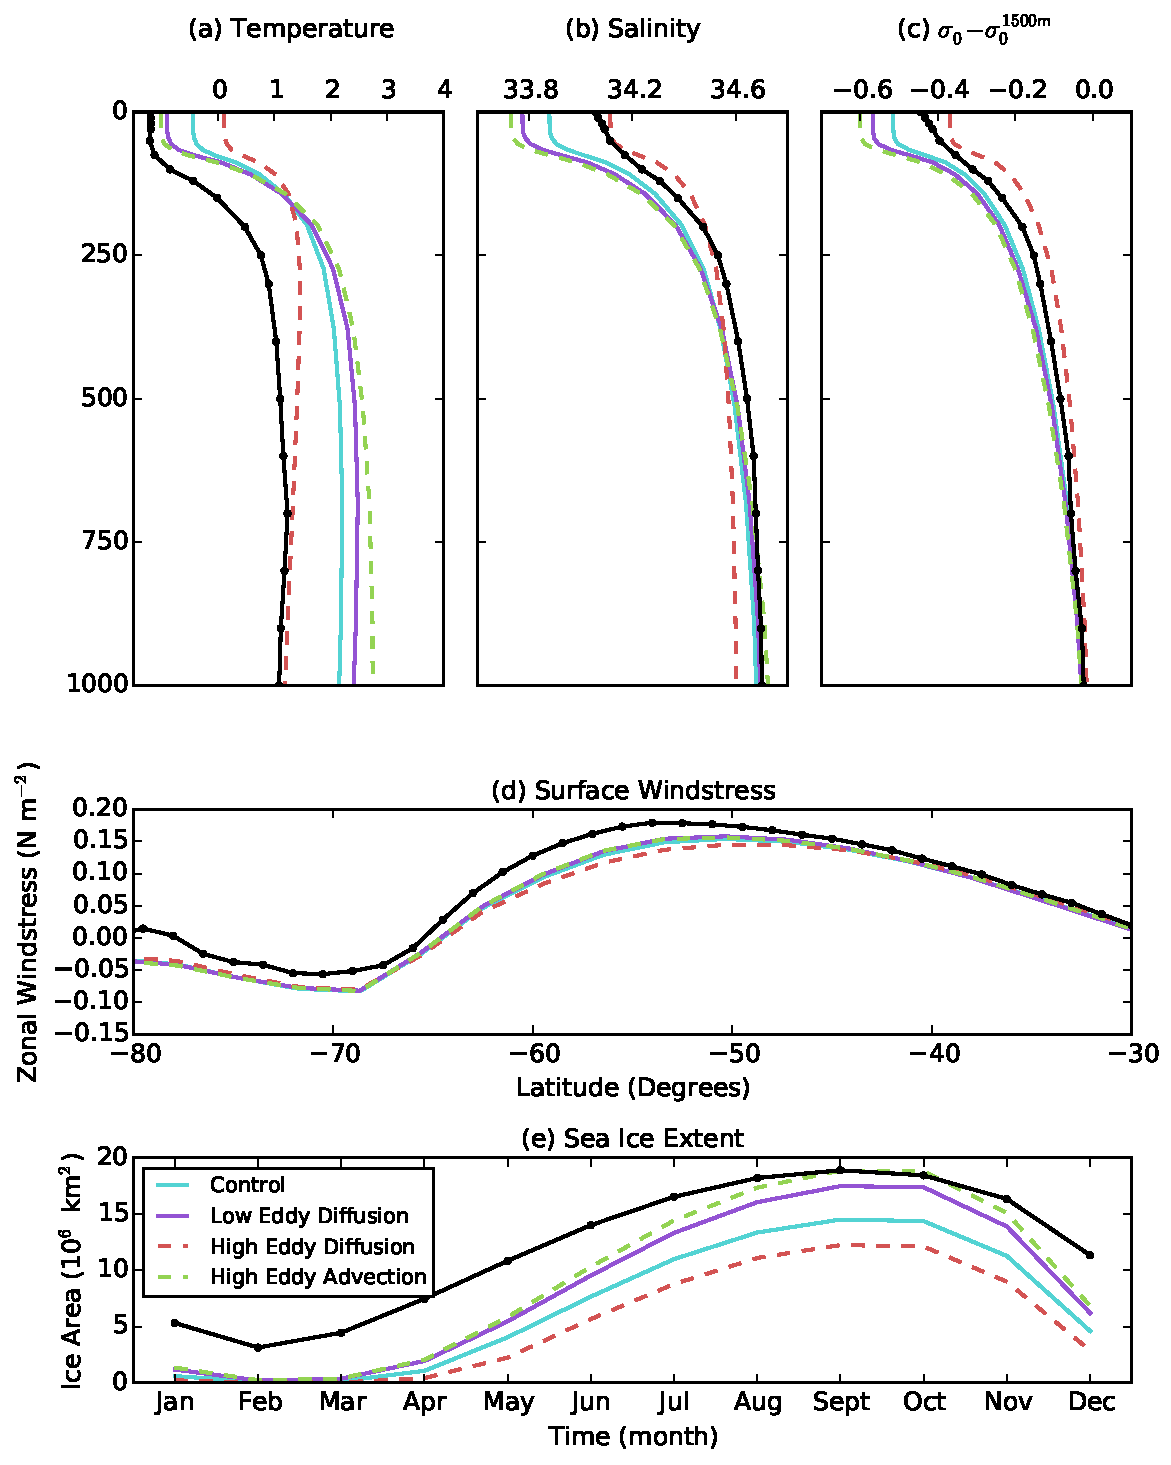
\includegraphics[width=33pc]{figure1.pdf}
\caption{Comparison of control (blue), low eddy diffusion (purple), high eddy
diffusion (red), and high eddy advection (green) simulations. JJA Southern Ocean
(60--90$^{\circ}$S) (a) temperature
(b) salinity and (c) density stratification
($\sigma_0 - \sigma_0^{\mathrm{1500m}}$). (d) JJA zonal surface wind stress
and (e) Antarctic sea ice extent. Observational data for each metric is shown in
black. Temperature, salinity, density stratification are estimates from the 2001
World Ocean Atlas 2001 dataset \citep{Boyer2002}. Surface wind stress are from ERA-Interim and averaged
between 1979--2015. Sea extent is calculated using the National Snow and Ice Data
Center Sea Ice Index \citep{Fetterer2016}}
\label{fig:climatology}
\end{figure}

The various $A_{\mathrm{redi}}$ simulations are discussed at length in
\citet{Pradal2014} and \citet{AnandGnanadesikan2015}, which examine the mean
climate response and sensitivity of anthropogenic carbon uptake to changing the
A$_{\mathrm{redi}}$ parameter. Here instead, we use the various simulations to
test the robustness of the mechanisms driving the co-variability of heat and
carbon. Because the different simulations have varying Weddell Sea  convective
variability (similar to the spread in CMIP5 models, see below), we can see if
convection alters the mechanisms driving the co-variability of heat and carbon
in this model. Unlike the CMIP5 suite where differences in biological models,
atmospheric radiation code, and sea ice formation contribute to intermodel
spread, our simulations differ only in the mesoscale parameterizations to
isolate the influence of Weddell Sea convection on the co-variability of heat
and carbon content.

\subsection{Heat and Carbon Content}
\label{subsection:Methods Heat and Carbon Content}
Heat and carbon content are calculated globally and regionally. The oceanic heat
content (H) is calculated using the subsurface potential temperature ($\theta$), and
integrated globally:

\begin{equation}
  H_{global} = \sum_{k = 0}^{bottom} \sum_{j = -90}^{90} \sum_{i=0}^{360} \rho
  c_p \theta \delta x_i \delta y_j \delta z_k
\end{equation}

Similarly, carbon content is calculated using Dissolved Inorganic Carbon (DIC)
concentration and integrated globally:

\begin{equation}
  C_{global} = \sum_{k = 0}^{bottom} \sum_{j = -90}^{90} \sum_{i=0}^{360} \rho
  [DIC] \delta x_i \delta y_j \delta z_k
\end{equation}

Because the oceanic heat and carbon reservoirs are so large ($150,000\times10^
{22}$ J and $37,000$ PgC, respectively), and the natural variability relatively
small ($\pm3\times10^{22}$ J and $\pm3$ PgC, respectively), we express the
variability as an anomaly from the climatological mean.

\subsection{Surface Heat Flux}
\label{subsection:Surface Heat Flux Analysis}

We determine the surface heat flux by vertically integrating the vertical
diffusion term over the entire water column and subtracting the geothermal heat
flux from the sea floor:
\begin{equation}
\begin{split}
\sum_{k = 0}^{bottom} {\bigg( \rho_k c_{p} {\bigg(\frac{\partial \theta}{\partial t}
\bigg)_{vdiff}}\bigg)_k}\delta z_k
 -… Q_{geo} = \\
Q_{SW} + Q_{LW} + Q_{latent} + Q_{sensible} = Q_{surface}
\end{split}
\end{equation}

The advantage to defining the surface heat flux with this method, as opposed to
the model-calculated surface heat flux, is that we can determine the heat
lost to overlying sea ice in addition to the atmosphere as well as track heat
sinks such as the melting of snow.

\begin{figure}
\centering
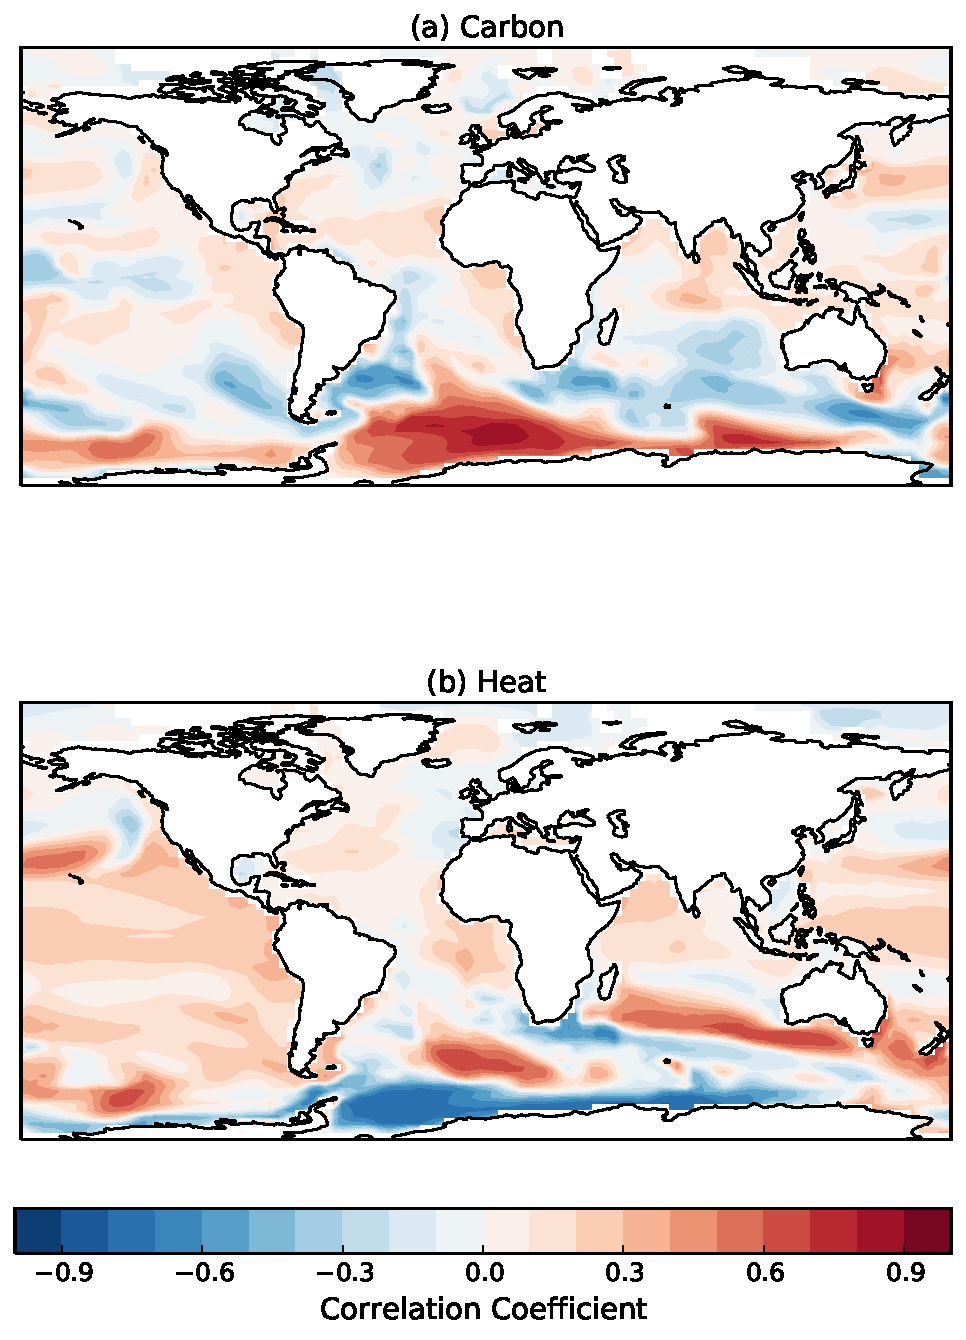
\includegraphics[width=19pc]{figure2.pdf}
\caption{Correlation between (a) vertically integrated carbon content at each
location and global carbon content and (b) vertically integrated heat content at
each location and global heat content for the control simulation
(A$_{\mathrm{redi}}$ = 800 m s$^{-2}$).}
\label{fig:heat_carbon_correlations}
\end{figure}

\subsection{Southern Ocean}
As has been previously documented \citep{DeLavergne2014a}, ESM2Mc has a
particularly active Southern Ocean. Deep convective events
occur often in the Southern Ocean, and have a sizable impact on the climate
system. \citet{Cabre} recently showed that Southern Ocean convective events in
this model have an impact on the Southern Hemisphere surface temperatures,
Hadley cell, and radiative balance. In light of the Southern Ocean influence in
this model, we first assessed the contribution of Southern Ocean variability to
global heat and carbon variability. Figure~\ref{fig:heat_carbon_correlations}
shows the correlation between vertically integrated carbon (heat) content at
each location with the global carbon (heat) content in the  \textit{control}
simulation. This initial analysis suggests the importance of  the Southern
Ocean, and particularly the Weddell Sea on global heat and carbon  variability
and will be more thoroughly examined in
section~\ref{section:Temporal and Spatial Variations in Heat and Carbon Content}.

%%%%%%%%%%%%%%%%%%%%%%%%%%%%%%%%%%%%%%%%%%%%%%%%%%%%%%%%%%%%%%%%%%%%%%%%%%%%%%%%
% RESULTS
%%%%%%%%%%%%%%%%%%%%%%%%%%%%%%%%%%%%%%%%%%%%%%%%%%%%%%%%%%%%%%%%%%%%%%%%%%%%%%%%
%% Section 1
\section{Temporal and Spatial Variations in Heat and Carbon Content}
\label{section:Temporal and Spatial Variations in Heat and Carbon Content}

%% Subsection 1

\subsection{Weddell Sea Convection}
In the mid-1970s, an anomalous opening in the sea ice in the Weddell Sea was
observed \citep{Carsey2009}. Named the Weddell Polynya, this large opening was
observed for three consecutive austral winters: 1974--1976. The polynya was
formed and maintained by vigorous convective mixing where the upward flux of
deep and relatively warm waters provided enough energy to melt the above sea
ice \citep{Gordon1982,Martinson1981}. This heat loss at the surface resulted in
subsurface cooling deep into the water column, depleting the subsurface heat
reservoir.

While a large feature like the Weddell Polynya has not been observed since and is considered to be a
rare event, these polynya events can be quite common in climate models. A recent
paper by \citet{DeLavergne2014a} quantifies these convective events in CMIP5
model preindustrial control simulations and shows the spread across models. They
find that some CMIP5 models have very little convection, while others have
constant deep convection, with most models lying somewhere in between.

Changing the mesoscale eddy parameterization in our model suite has a large
impact on the Weddell Sea deep convection. Figure~\ref{fig:convection} shows the
annually-averaged subsurface temperature as a function of time (colored
contours) and the annual mixed layer depth (black line) averaged over the
Weddell Sea (60--80$^{\circ{}}$S, 60$^{\circ{}}$W--0). The downward spikes in
mixed layer depth, and the concurrent decline in subsurface temperature indicate
the occurrence of a deep convective event. The simulations range from no
convection in the \textit{high eddy advection simulation} (Figure
~\ref{fig:convection} (d)), to constantly convecting in the \textit{high eddy
diffusion simulation} (Figure~\ref{fig:convection} (c)), with the
\textit{control} and \textit{low eddy diffusion} cases oscillating between
convective and non-convective periods (Figure~\ref{fig:convection} (a) and (b)).

When the neutral diffusion coefficient (A$_{\mathrm{redi}}$) is increased as in
the \textit{high eddy diffusion} simulation, the along isopycnal diffusive
mixing is increased. In the Southern Ocean where the isopycnals slope up to the
surface and the subsurface water is warmer than the surface ocean, this
increased along-isopycnal diffusion acts to decrease the vertical gradient in
temperature and salinity (also shown in Figure~\ref{fig:climatology} (a) - (c)).
This results in a lower subsurface temperature,
a weaker density contrast between deep and surface waters, less subsurface heat
build-up, and no large convective `events'
(Figure~\ref{fig:convection} (c)). Alternatively, a lower  neutral
diffusion coefficient as in the \textit{control} and \textit{low eddy diffusion}
simulations does the opposite: the along-isopycnal diffusive mixing is decreased
and subsurface heat is able to build up until a deep convective event occurs
(Figure~\ref{fig:convection} (a) and (b)).

Changing the eddy advection coefficient
(A$_{\mathrm{GM}}$) on the other hand impacts the slope of the isopycnal
surfaces. As shown in \citet{Gent2010d}, increasing A$_{\mathrm{GM}}$ acts to
flatten the isopycnal surfaces and reduce vertical exchange. In the Southern
Ocean where the isopycnals slope up to the surface, and the A$_{\mathrm{GM}}$
value is usually small, increasing the minimum value of A$_{\mathrm{GM}}$ thus
reinforces the vertical density gradient. The result is a build-up of subsurface
heat that continues to grow throughout the \textit{high eddy advection}
simulation. The reinforced density gradient is strong enough to suppress deep
convection throughout the 500-year simulation (Figure~\ref{fig:convection} (d)).

It is important to note that while the existence of subsurface heat build-up is
known to be important for the existence of deep convective events, it is not yet
known what mechanism initiates deep convection in the model or sets the
timescales for convective variability. We have found, however, that by changing
these parameterizations, we are able to span the range of convective variability
seen in CMIP5 models as shown in \citet{DeLavergne2014a} without the
additional complications introduced by different representations of atmospheric
processes and biological cycling. In this paper we will use these different
convective states of the model to identify the impact convective variability has
on both carbon and heat in the Southern Ocean and globally.


\begin{figure}
\centering
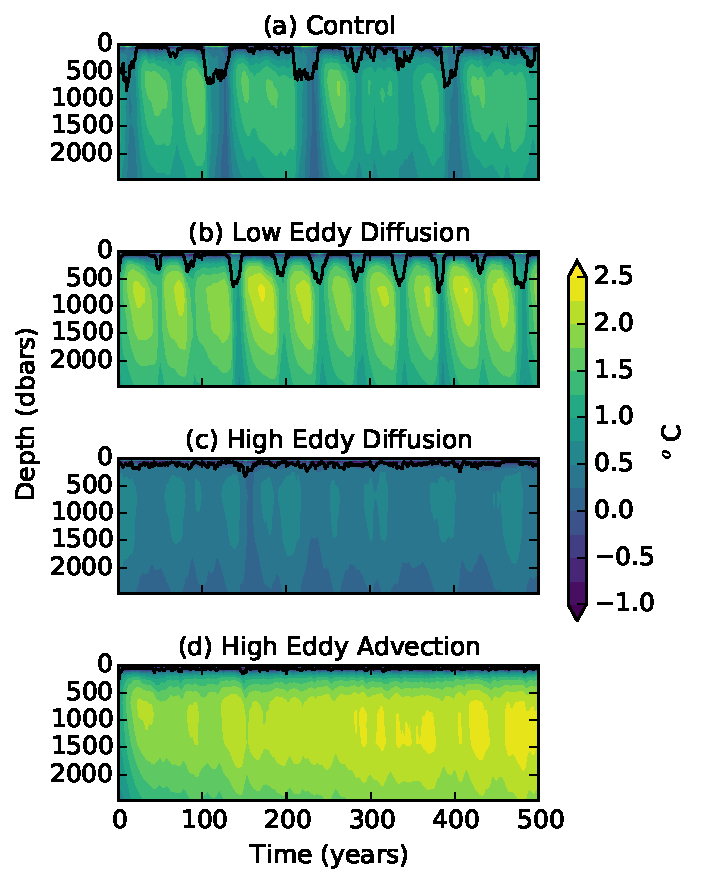
\includegraphics[width=19pc]{figure3.pdf}
\caption{Annually averaged subsurface temperature (color contours) and mixed
layer depth (solid black line) averaged over Weddell Sea for (a) Control
simulation (A$_{\mathrm{redi}}$ = 800 m s$^{-2}$), (b) Low Eddy Diffusion simulation
(A$_{\mathrm{redi}}$ = 400 m s$^{-2}$), (c) High Eddy Diffusion simulation
(A$_{\mathrm{redi}}$ = 2400 m s$^{-2}$), and (d) High Eddy Advection simulation
(GM$_{\min}$ = 600 m s$^{-2}$).}
\label{fig:convection}
\end{figure}

\subsection{Global Heat and Carbon Variability}
We first aim to understand the variability in global oceanic heat and carbon
content in the \textit{control} simulation. The time-series of global carbon and
heat content anomaly is shown in Figure~\ref{fig:heat_carbon_convection} (a) and
(b). Both quantities show strong multi-decadal-scale variability, undergoing
strong fluctuations roughly every 50 years. The magnitude of global
carbon variability is about $\pm$ 3 PgC which accounts for only approximately
3\% of the estimated anthropogenic uptake of carbon over the past few decades
\citep{Khatiwala2012,Sabine2004,Waugh2006}. The variability in global heat
content on the other hand is about $\pm$ 3 $\times 10^{22}$ J. This is a much
larger percentage (20\%) of the estimated uptake of anthropogenic in heat recent
decades \citep{Levitus2009}. Figure~\ref{fig:heat_carbon_convection}
(c) shows the time-series of Weddell Sea (WS)
subsurface temperature (averaged between 1500 m and 2500 m). This quantity has
been shown to be a good proxy for WS deep convection since the subsurface
temperature is significantly decreased during convective events \citep{Bernardello2014}.
Comparing the time-series of the WS subsurface temperature to those of
global heat and carbon anomalies, it is apparent that there is a strong
relationship. In the control simulation, the WS subsurface temperature explains
61\% and 35\% ($r^2$) of the variance in global heat content and carbon content
respectively (Table~\ref{t1}), with the strongest correlation occurring at time
lag = 0. The correlation between WS subsurface temperature and global heat and
carbon content is also high for the \textit{low eddy diffusion} simulation,
while the relationship is less strong (yet significant) for the \textit{high
eddy diffusion} and \textit{high eddy advection} simulations (Table~\ref{t1}).
These results suggest that WS convection is closely tied to the global heat and
carbon content.

\begin{figure}
\centering
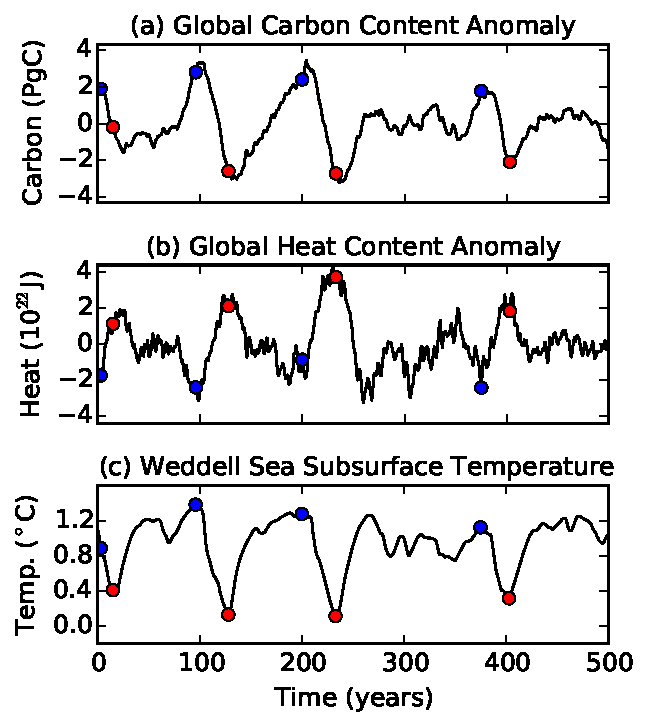
\includegraphics[width=19pc]{figure4.pdf}
\caption{Carbon content anomaly, heat content anomaly and Weddell Sea subsurface
temperature (averaged between 1500--2000 m, 0$^{\circ}$--60$^{\circ}$W,
60$^{\circ}$--80$^{\circ}$S) for control simulation. Blue circles indicate
beginning of convection and red circles indicate end of convection defined using
four strongest local maxima and minima in Weddell Sea Subsurface Temperature.}
\label{fig:heat_carbon_convection}
\end{figure}


\begin{table}[h]
\caption{Relationship between Weddell Sea subsurface temperature and global carbon
and heat content anomalies. All correlations are statistically significant from
0 (p = 0.005).}\label{t1}
\begin{center}
\begin{tabular}{lcc}
\hline
Simulation              & Carbon Content & Heat Content \\
\hline
 & \multicolumn{2}{c}{\textit{Correlations (r)}} \\
Control & 0.59 & -0.79   \\
Low Aredi & 0.61 & -0.56  \\
High Aredi & 0.49 & -0.20 \\
High GM$_{\mathrm{min}}$ min     & 0.12 & -0.24   \\
\end{tabular}
\end{center}
\end{table}

The global heat and carbon content anomaly time-series for all simulations is
shown in Figure~\ref{fig:heat_carbon_ts}. The
magnitude and frequency of heat and carbon content variability changes
substantially across the different simulations.  Comparing the time-series
of global carbon content and heat content anomalies in the control simulation we
find that they are anti-correlated ($r=-0.629$, Figure~\ref{fig:corr_coeff}).
Given that in this model, the global heat and carbon are primarily driven
by Southern Ocean variability and Southern Ocean convection acts to deplete the
Southern Ocean of both carbon and heat content, we would expect that global heat
and carbon content should vary together. Therefore it is surprising that the two
quantities are so strongly negatively correlated.

\begin{figure}
\centering
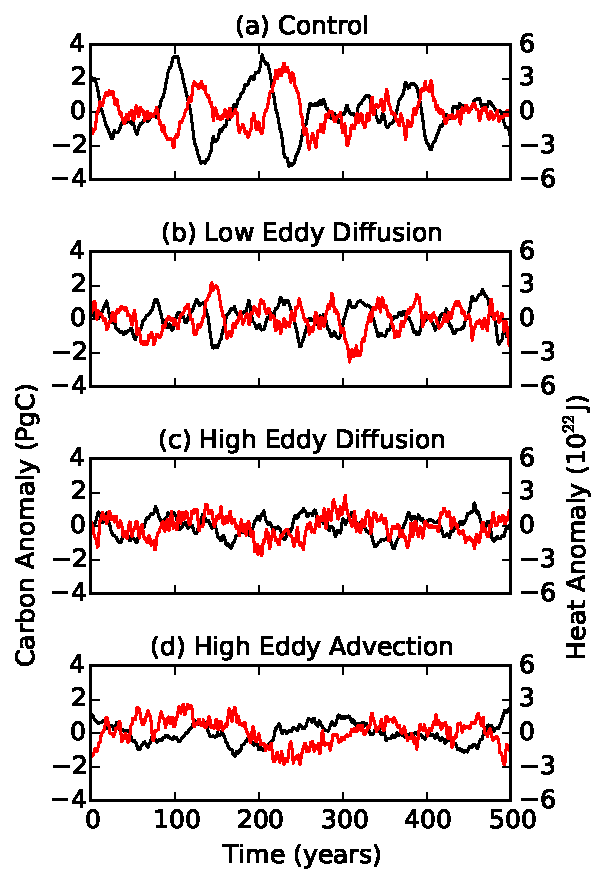
\includegraphics[width=19pc]{figure5.pdf}
\caption{Globally integrated carbon content anomaly (black) and heat content
anomaly (red) for (a) Control
simulation (A$_{\mathrm{redi}}$ = 800 m s$^{-2}$), (b) Low Eddy Diffusion simulation
(A$_{\mathrm{redi}}$ = 400 m s$^{-2}$), (c) High Eddy Diffusion simulation
(A$_{\mathrm{redi}}$ = 2400 m s$^{-2}$), and (d) High Eddy Advection simulation
(GM$_{\min}$ = 600 m s$^{-2}$).}
\label{fig:heat_carbon_ts}
\end{figure}

This anti-correlation relationship between global heat and carbon content is
consistent in the additional simulations as well (Figure~\ref{fig:heat_carbon_ts}).
Figure~\ref{fig:corr_coeff} shows the Pearson
correlation coefficient between global heat and carbon content for each
simulation. All of the simulations have a statistically significant negative
correlation between global heat and carbon exceeding -0.3. The two simulations
which oscillate between convective and non-convective periods (\textit{control} and \textit{low eddy
diffusion}) have stronger correlations at or exceeding -0.5. The fact that
significant anti-correlation is found for all simulations suggests that
the mechanisms causing this anti-correlation in global heat and carbon content
are not strongly dependent on the convective state in the WS.

\begin{figure}
\noindent
\centering
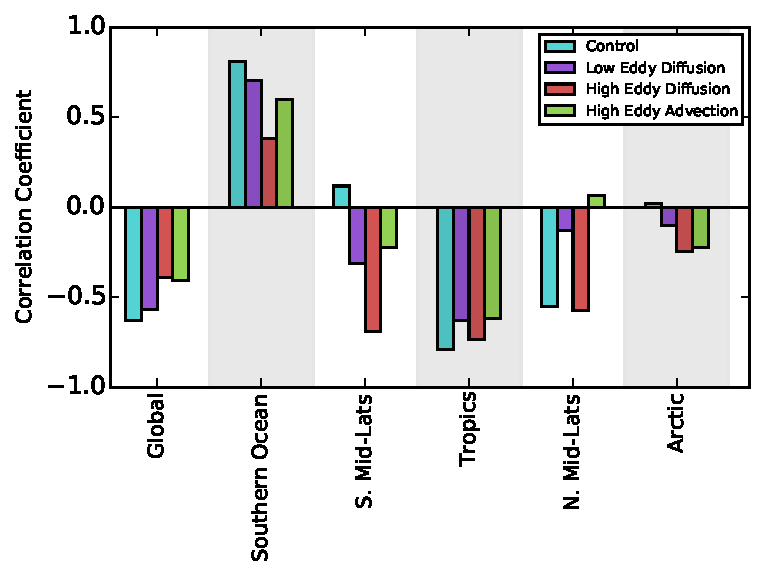
\includegraphics[width=33pc]{figure6.pdf}
\caption{Pearson correlation coefficients for integrated carbon content anomaly
versus integrated heat content anomaly for each region.}
\label{fig:corr_coeff}
\end{figure}

In light of these results, we find it helpful to divide these simulations up
into two classes: the \textit{low mixing simulations} which oscillate between
convective and non-convective periods (control and low eddy diffusion) and the
\textit{high mixing simulations} simulations which do not (high eddy diffusion
and high eddy advection). The low mixing simulations are characterized by a
build-up and subsequent release of abyssal heat content in the Southern Ocean
(Figure~\ref{fig:convection}). These two simulations also have very strong
oscillations in the global heat and carbon content, closely linked to the WS
convection. The high mixing simulations on the other hand do not show
this oscillation between subsurface build-up and release in the Southern Ocean,
but rather either constant depletion in subsurface temperature in the
\textit{high eddy diffusion} (Figure~\ref{fig:convection} (c)) or a constant
build-up of subsurface temperature in the \textit{high eddy advection}
(Figure~\ref{fig:convection} (d)). The lack of these oscillating convective
states results in smaller global heat and carbon variability
(Figure~\ref{fig:heat_carbon_ts}), and a weaker relationship (although
significant) between the WS and the global heat and carbon content.

To understand why the global heat and carbon are strongly anti-correlated, next
we look at the regional relationships between heat and carbon content.


%% Subsection 2
\subsection{Regional Heat and Carbon Variability}
To diagnose which regions significantly contribute to the observed variability
in global heat and carbon content, we break the global ocean into zonal bands:
the Southern Ocean (90$^o$S--55$^o$S), the southern mid-latitudes (55$^o$S--
20$^o$S), tropics (20$^o$S--20$^o$N), the northern mid-latitudes (20$^o$N--
60$^o$N), and the Arctic (60$^o$N--90$^o$N). These divisions were defined by the
zonal average of the zero wind-stress curl in order to isolate the dynamical
regions (not shown). The correlation coefficients
between heat and carbon content in each of these regions are also shown in
Figure~\ref{fig:corr_coeff}. The correlation coefficients give a sense of what
remains consistent across the simulations even with the different convective
states. The Southern Ocean has a strong positive correlation between heat and
carbon for all the simulations. Additionally, in the tropics there is a strong
negative correlation between heat and carbon for all the simulations. This
result suggests that the negative correlation in the tropics is key to
understanding the negative correlation between heat and carbon seen globally.

To get a better sense of which regions dominate the variability, we decompose
the global heat and carbon regionally by regressing the regional inventories of
heat and carbon against the global inventories of heat and carbon. We first
consider heat content in the \textit{control} simulation
(Figure~\ref{fig:linear_regression} (a), red dots). The regression highlights
the importance of three regions in contributing to the global heat content
signal: the Southern Ocean, southern mid-latitudes, and tropics. The Southern
Ocean regression coefficient has a magnitude similar to the southern
mid-latitudes and tropics, but the opposite sign. This indicates that the
variability in Southern Ocean heat content is being compensated by similar
magnitude variability in heat content in both the southern mid-latitudes and
tropics.

\begin{figure}
\noindent
\centering
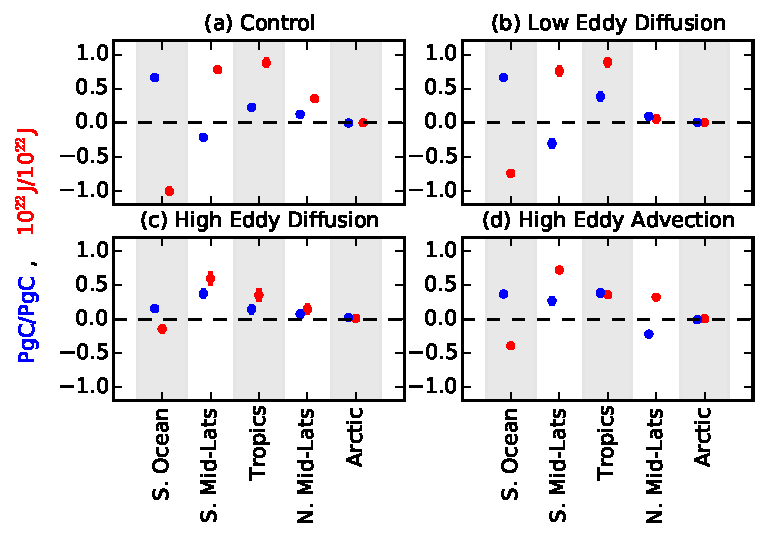
\includegraphics[width=33pc]{figure7.pdf}
\caption{Linear regression of each region's carbon content against global carbon
content (blue) and each regions heat content against global heat content (red).
Linear regression  95\% confidence interval is shown, but too small to be
discerned.}
\label{fig:linear_regression}
\end{figure}

The picture is nearly identical in the \textit{low eddy diffusion} simulation
(which also undergoes oscillations between convective and non-convective
states). The Southern Ocean heat content variability is compensated by similar
magnitude variability in both the southern mid-latitudes and tropics
(Figure~\ref{fig:linear_regression} (b)). However, the \textit{high mixing}
simulations are less clear. The regional heat content is dominated by the
southern mid-latitudes with weak compensation between the Southern Ocean
and tropics (Figure~\ref{fig:linear_regression} (c) and (d)).

The linear regression of regional carbon content
(Figure~\ref{fig:linear_regression}, blue dots), however, suggests that the
Southern Ocean carbon content variability contributes most towards the global
carbon content variability for all simulations. For the \textit{low mixing simulations},
there appears to be a compensation between the southern mid-latitude and tropical
carbon content variability. This compensation in regional variability is not seen
in the \textit{high mixing simulations} where the regression coefficients are both
positive for these two regions. Regardless of these differences, the Southern
Ocean is the region with the largest regression coefficient for all simulations.

The time-series of the regional variability for heat and carbon content compared
to the global heat and carbon content are shown in the supplemental information
as an additional way to visualize the offsetting variations in different regions.

This relationship between WS deep convection and Southern
Hemisphere surface warming is consistent with \citet{Bernardello2014} and
\citet{Cabre}. Both papers use the same GFDL model shown here in the control configuration to assess the
impact of convection on the climate system and both sets of analysis show
similar Southern Hemisphere surface warming in response to a convective event.
Specifically, \citet{Cabre} show that during these winter time convective events,
substantial warming occurs in the Southern Ocean, increasing sea surface
temperatures, decreasing sea ice and low clouds, and increasing solar radiation
absorption. The result is a substantial warming of the Southern Hemisphere surface
ocean and atmosphere. This atmospheric warming propagates to the rest of the
atmosphere almost instantaneously, changing the meridional temperature gradient
and altering the strength of the Hadley Cell in both hemispheres. For a more
detailed look at the teleconnections between the Southern Ocean convection and
tropical SST increases, we refer the reader to \citet{Cabre}.


\begin{figure}
\noindent
\centering
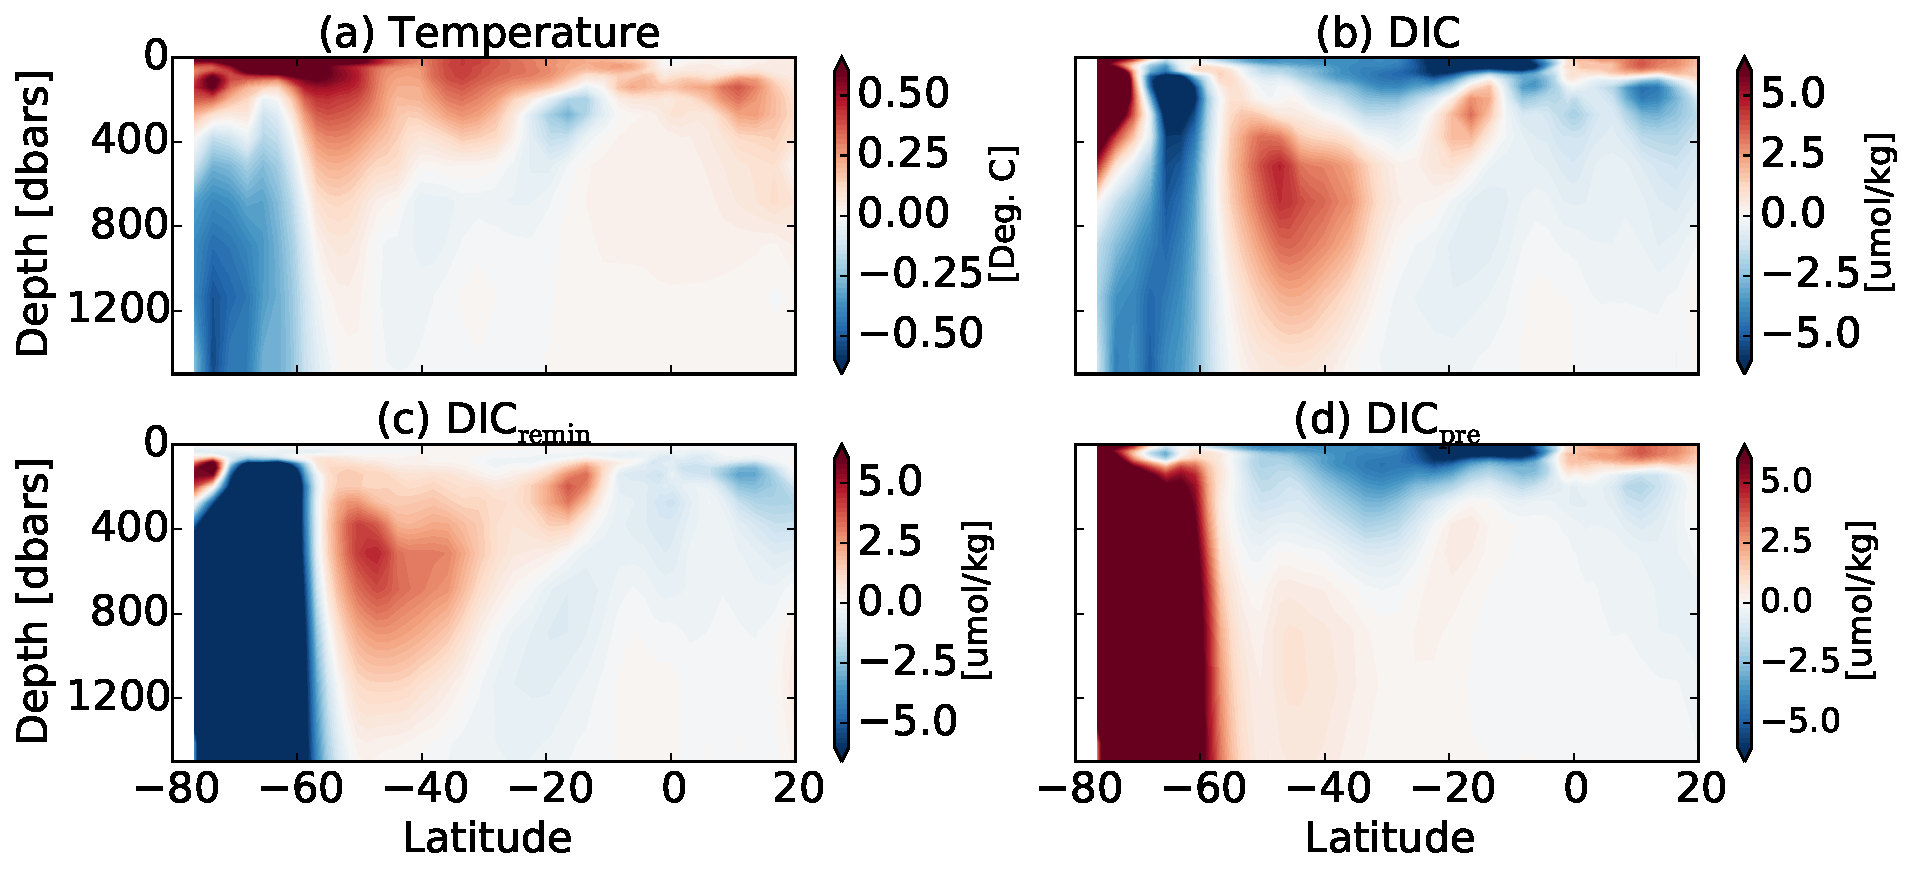
\includegraphics[width=33pc]{figure8.pdf}
\caption{Subsurface (a) potential temperature, (b) DIC, (c) remineralized DIC, and (d) preformed
DIC for convective year composite from control simulation. Only the surface ocean
is shown to highlight the strongest-magnitude features.}
\label{fig:subsurface}
\end{figure}



%%%%%%%%%%%%%%%%%%%%%%%%%%%%%%%%%%%%%%%%%%%%%%%%%%%%%%%%%%%%%%%%%%%%%%%%%%%%%%%%
% MECHANISMS
%%%%%%%%%%%%%%%%%%%%%%%%%%%%%%%%%%%%%%%%%%%%%%%%%%%%%%%%%%%%%%%%%%%%%%%%%%%%%%%%
\section{Mechanisms Driving Variability}
\label{section:Mechanisms}

In order to understand why global heat and carbon content are anti-correlated
we look more in depth at the mechanisms driving the regional variability of
these quantities.

\subsection{Heat Content Variability}
We first examine the variability of heat content. As shown for the \textit{control}
simulation subsurface temperature in Figure~\ref{fig:subsurface} (a), convection
acts to deplete the Southern Ocean of subsurface heat, and increase the surface
heat content in the southern mid-latitudes and tropics. These processes are more
explicitly shown in Figure~\ref{fig:heat_flux_fig}. Periods of convection
(highlighted in grey) are consistent with deepening of the mixed layer
(black line), a depletion of subsurface Southern Ocean temperature (green line),
an increase in Southern Ocean heat flux into the atmosphere (negative out of
ocean -- red line), and an increase in southern mid-latitude and tropical SST
(blue line). These processes are consistent in the \textit{low eddy diffusion}
simulation which  also oscillates between convective and non-convective periods
(not shown).

This relationship between WS deep convection and Southern
Hemisphere surface warming is consistent with \citet{Bernardello2014} and
\citet{Cabre}. Both papers use the same GFDL model shown here to assess the
impact of convection on the climate system and both sets of analysis show
similar Southern Hemisphere surface warming in response to a convective event.
Specifically, \citet{Cabre} show that during these winter time convective events,
substantial warming occurs in the Southern Ocean, increasing sea surface
temperatures, decreasing sea ice and low clouds, and increasing solar radiation
absorption. The result is a substantial warming of the Southern Hemisphere surface
ocean and atmosphere. This atmospheric warming propagates to the rest of the
atmosphere almost instantaneously, changing the meridional temperature gradient
and altering the strength of the Hadley Cell in both hemispheres. For a more
detailed look at the teleconnections between the Southern Ocean convection and
tropical SST increases, we refer the reader to \citet{Cabre}.

In this paper we show that the impact of this surface warming in the southern
mid-latitudes and tropics is strong enough to counteract the depletion of
subsurface heat in the Southern Ocean, resulting in a global increase in heat
content after WS convection.

\begin{figure}
\noindent
\centering
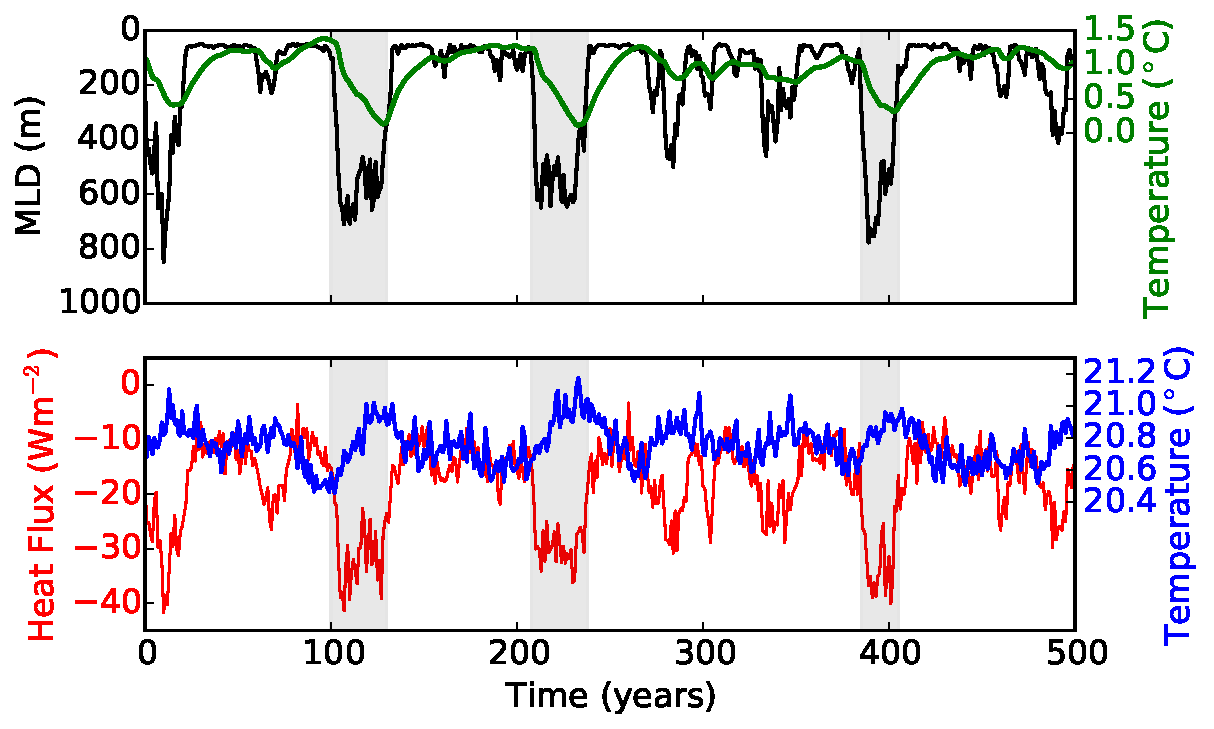
\includegraphics[width=33pc]{figure9.pdf}
\caption{Top: Weddell Sea subsurface temperature as in Figure
~\ref{fig:heat_carbon_convection} (green) and Weddell Sea mixed layer depth
(black). Bottom: Southern Ocean surface heat flux where positive indicates into
the ocean (red), Southern Hemisphere SST averaged between
0$^{\circ}$--55$^{\circ}$S (blue) for the control simulation.}
\label{fig:heat_flux_fig}
\end{figure}

\subsection{Carbon Content Variability}
Next we examine the regional mechanisms driving variability in carbon content in
order to understand the anti-correlation between global heat and carbon content.
Examining the \textit{control} simulation (Figure~\ref{fig:subsurface} (b)), we
see that during convection there is a strong subsurface depletion of DIC in the
Southern Ocean, an increase in subsurface DIC in the southern mid-latitudes, and
a further depletion of surface-layer DIC in the southern mid-latitudes to equator.
To understand these spatial patterns, we
break the DIC up into two components:
\begin{equation}
DIC = DIC_{pre} + DIC_{remin}
\end{equation}

where the preformed component (DIC$_{pre}$) is the DIC concentration of the
water at the ocean surface and the remineralized component (DIC$_{remin}$) is
the carbon concentration due to biological accumulation. DIC$_{pre}$ is set
equal to DIC in the mixed layer and is advected and mixed into the ocean
interior with biological sources and sinks set to zero. Thus by definition,
 DIC$_{remin}$ is zero within the mixed layer and represents the component of
 DIC in the interior that is due to biological sources and sinks.

When breaking the DIC down into its two components, we see that in
the Southern Ocean there is a very strong depletion of subsurface remineralized
carbon and a strong increase in preformed carbon (Figure~\ref{fig:subsurface}
(c) and (d)). This signal is consistent with deep convective mixing. The
increase in subsurface DIC$_{pre}$ occurs from mixing relatively high surface
DIC$_{pre}$ down into the subsurface and the decrease in DIC$_{remin}$ occurs from
mixing relatively high DIC$_{remin}$ from the subsurface to the surface layer.
Mixing these high DIC waters from the abyssal Southern Ocean to the surface
results in outgassing of CO$_2$ to the atmosphere (not shown) and the net result
is a reduction in subsurface DIC.

The depletion in surface DIC in the Southern Hemisphere tropical region on the
other hand is entirely due to a depletion in preformed DIC. This region also
experiences a strong warming thus reducing the solubility of CO$_{\mathrm{2}}$
within the surface waters and
limiting the amount of DIC that can be held by the water in equilibrium with the
atmosphere and at constant alkalinity. To verify that the reduction
in solubility is driving the subsequent decrease in DIC, we show the
DIC content versus heat content for the tropical region in
Figure~\ref{fig:heat_dicpre_scatter} (a). The strong negative relationship
supports the hypothesis that the variability in preformed DIC in this region is
driven by changes in solubility. Figure~\ref{fig:heat_dicpre_scatter} (a)
additionally shows the theoretical change in carbon content given a change in
heat content due to solubility alone (constant pCO$_{\mathrm{2}}$ and alkalinity
-- black line) with a slope of  -0.27 PgC/$10^{22}$J. This relationship is calculated using the relationship derived
in \citet{Gruber1996} and scaled to relate carbon content with heat content.
There is good agreement between this theoretical model and the linear regression of carbon content
versus heat content for this region, represented by the dashed grey line (linear slope
values, $m$, also shown on Figure~\ref{fig:heat_dicpre_scatter}),
 further supporting the hypothesis that carbon variability is consistent
with variability in solubility.

\begin{figure}
\noindent
\centering
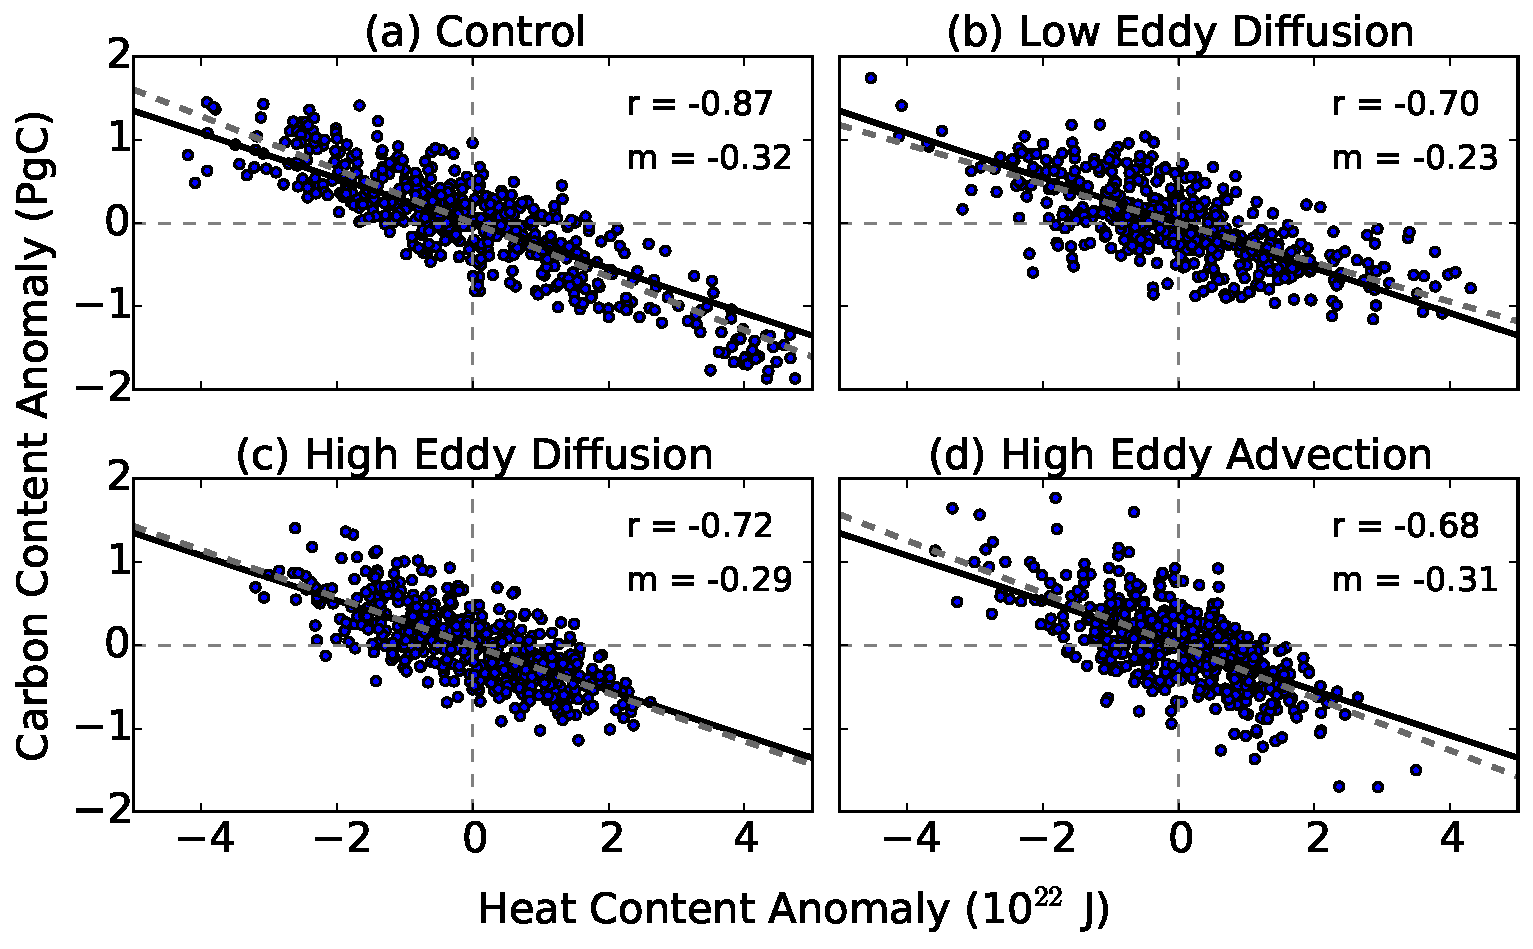
\includegraphics[width=33pc]{figure10.pdf}
\caption{Scatter of heat content anomaly vs preformed DIC integrated over the
tropical region for each simulation. Dashed grey linear line represents the linear fit of the carbon vs heat data with
slope, $m$, and pearson correlation coefficient $r$.
Solid black linear line represents the projected change
in carbon content given a change in heat content with constant alkalinity and
pCO$_2$ in equilibrium with the preindustrial atmosphere (scaled from \citet{Gruber1996}).
}
\label{fig:heat_dicpre_scatter}
\end{figure}

The above solubility mechanism appears to hold in all simulations
(Figure~\ref{fig:heat_dicpre_scatter} (b) -- (d)). All simulations have the same
negative relationship between preformed carbon content and heat content
integrated over the tropical region (20$^\circ{}$S -- 20$^\circ{}$N) with good
agreement with the scaled solubility line (black line). This result
suggests that the variability in DIC in this region is driven by variability
in the temperature-driven solubility, regardless of the high-latitude convective
variability.

Finally we examine the southern mid-latitude subsurface increase in DIC seen in
Figure~\ref{fig:subsurface} (b). Looking at the components of DIC, it is apparent that this
increase is entirely due to remineralized DIC. To understand why this increase
of remineralized DIC occurs, we correlate the remineralized DIC anomaly with ideal age
in the southern mid-latitude subsurface region (averaged between 40$^\circ{}$--
50$^\circ{}$S and 200--1000 m, Figure~\ref{fig:dic_remin_vs_age}). The ideal age
is a tracer in the model simulation which quantifies the mean time since the
water last had contact with the surface. The tracer is set to zero in the mixed
layer and ages at a rate of 1 yr yr$^{-1}$ after it leaves the mixed layer.
In all simulations, the remineralized DIC anomaly in this region is strongly correlated
with ideal age with Pearson
correlation coefficients exceeding 0.8 (Figure~\ref{fig:dic_remin_vs_age}).
Calculating the linear regression coefficient ($m$) between the remineralized
DIC and ideal age yields a rate of accumulation of remineralized DIC of
approximately 0.25 $\mu$mol kg$^{-1}$ yr$^{-1}$ for all simulations
(Figure~\ref{fig:dic_remin_vs_age}).
Comparing this rate of accumulation of remineralized DIC to the modeled local
remineralization rate ($jPO_4 \times$ 108 = 1.6 $\mu$mol kg$^{-1}$ yr$^{-1}$) we find that
the rate of accumulation of remineralized DIC in this region is significantly
less than the remineralization rate. The DIC found at a given point has
accumulated along many trajectories, some largely passing through surface waters
where the local remineralization rate is large, and some passing through deep
waters where the local remineralization rate is small. The low slope of the
relationship between DIC$_{remin}$ and age suggests that it is changes in the
fraction of waters taking deeper trajectories that is most important in
explaining the changes in Figure~\ref{fig:dic_remin_vs_age}.

\begin{figure}
\noindent
\centering
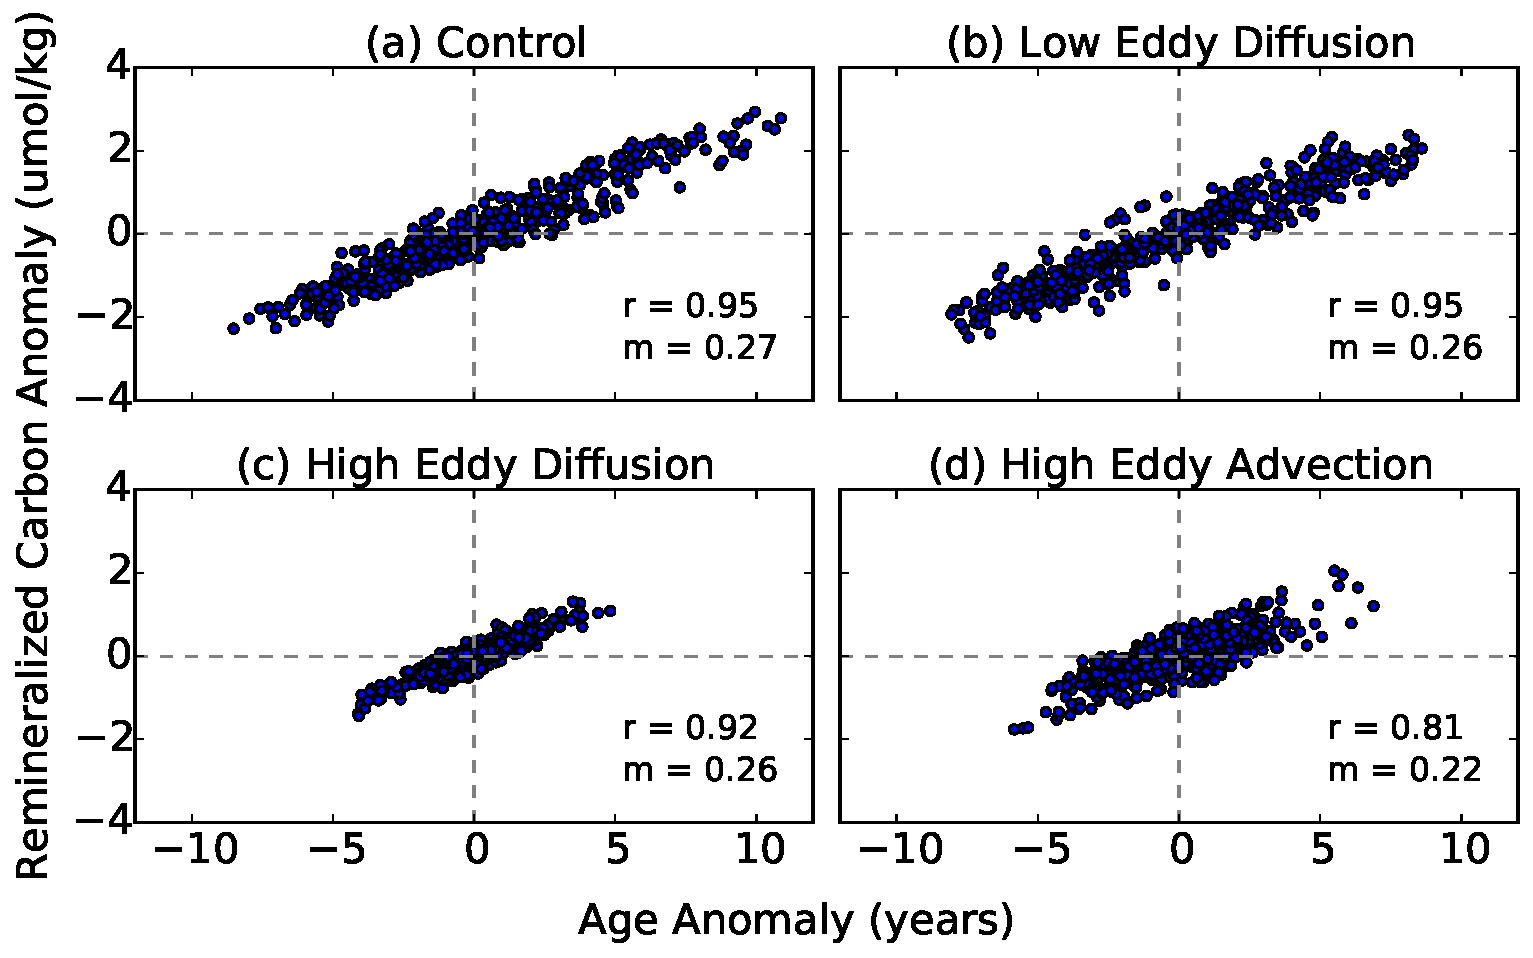
\includegraphics[width=33pc]{figure11.pdf}
\caption{Ideal age versus remineralized DIC for all simulations. Quantities are
averaged over latitudes 40$^{\circ}$--50$^{\circ}$S and 200--1000 m. Linear
regression coefficients, $m$, and pearson correlation coefficients, $r$, are
included for reference. }
\label{fig:dic_remin_vs_age}
\end{figure}

Because only changes in transport cause the ideal age to change, the strong
correlation between the remineralized DIC and ideal age suggest the accumulation
of DIC$_{remin}$ is due to a slow down of exchange between the surface and
subsurface waters. This conclusion is only valid if the rate of local
remineralization is constant, or does not impact the time tendency of DIC in
this region. Correlation analysis between the modeled remineralization rate and
DIC tendency suggest no significant (or very small) correlation between the two
variables (see supplemental material Figure 5) indicating the variability in
subsurface DIC$_{remin}$ is indeed due to variability in transport.

To verify that the same spatial relationship of DIC and its components is
consistent in all simulations, we show the covariance of globally integrated DIC
against zonally (and vertically) integrated DIC, DIC$_{pre}$, and DIC$_{remin}$
in Figure~\ref{fig:covariance}. The general pattern of covariance between the
global DIC and remineralized DIC shows a strong positive value in the Southern
Ocean followed by a decreasing to negative covariance in the southern mid-latitudes
and then increasing again to above zero in the tropics. This pattern is apparent
in all simulations, but with different magnitudes due to the different convective
variability. When comparing with Figure~\ref{fig:subsurface} it
is important to note that these covariance calculations use the DIC integrated
over the entire water column, whereas Figure~\ref{fig:subsurface} only shows the
surface layer (top 1500 dbars). Due to deep spreading of decreased DIC$_{remin}$
values from the Southern Ocean convection into the abyssal mid-latitudes (supplemental
Figure S6),
the depth-integrated global DIC and remineralized DIC covariance does not become
negative until approximately 45$^{\circ}$S.



\begin{figure}
\noindent
\centering
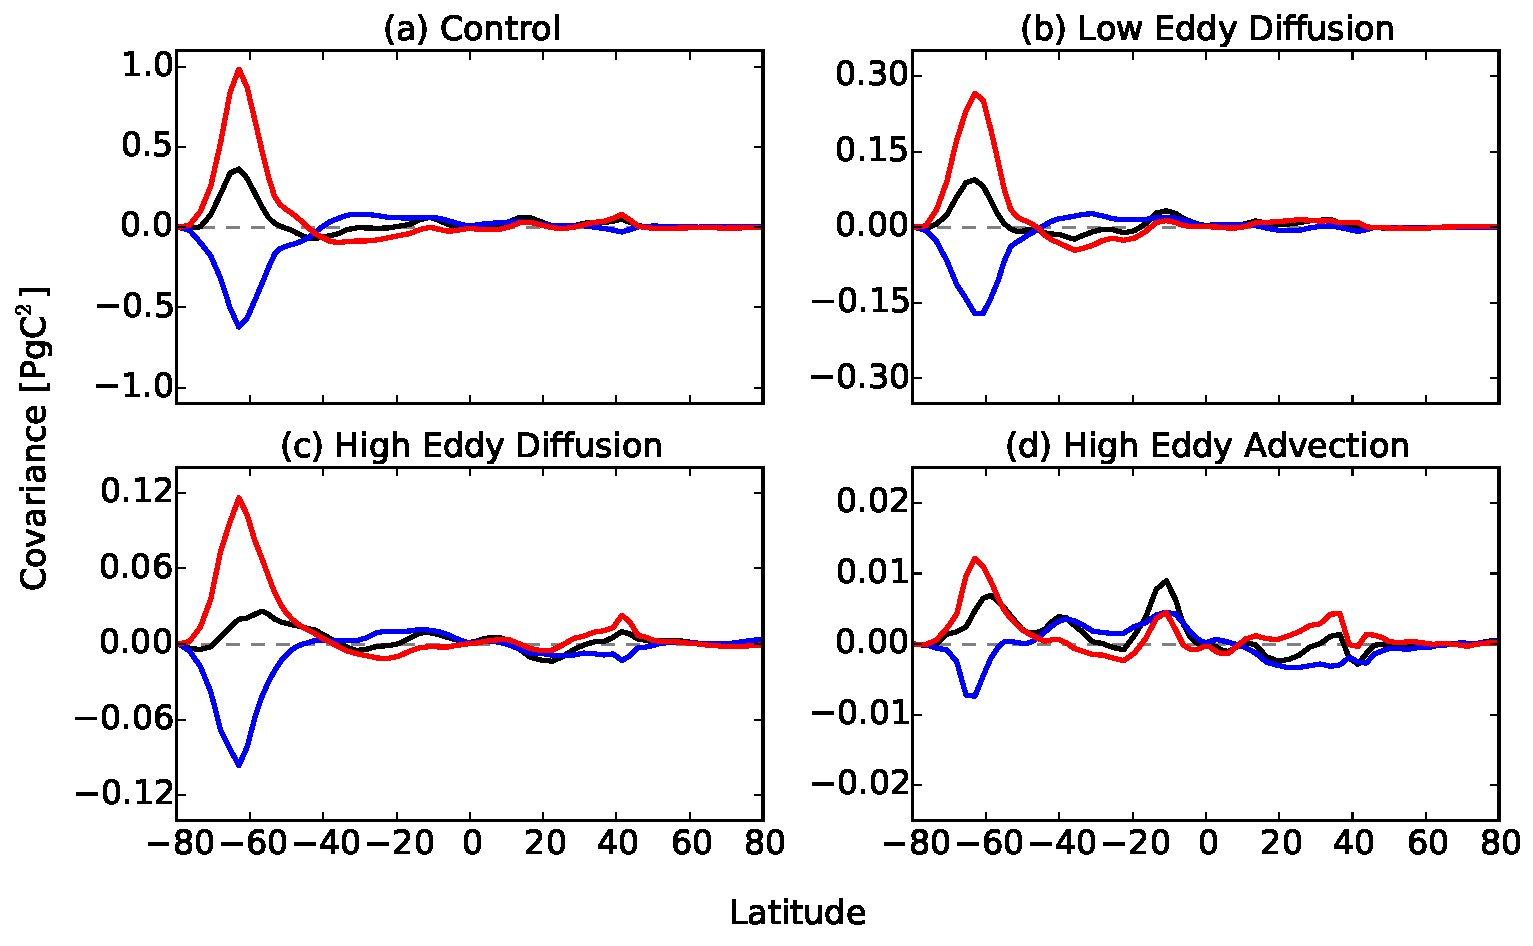
\includegraphics[width=33pc]{figure12.pdf}
\caption{Covariance between globally integrated DIC content and DIC (black),
preformed DIC (blue) and remineralized DIC (red) for each simulation as a
function of latitude. Note different y-axis scales.}
\label{fig:covariance}
\end{figure}

The opposite pattern holds for the covariance between global DIC
and preformed DIC: a negative covariance in the Southern Ocean, followed
by an increase in covariance in the southern mid-latitudes and a decrease below
zero north of the equator. Because of the lack of deep convection in the
\textit{high mixing simulations}, the Southern Ocean covariance is significantly smaller
than the other simulations (note different y-axis scales in
Figure~\ref{fig:covariance}), but the qualitative relationship remains the same.
The consistency in the general shape of these relationships suggests that the
same mechanisms are controlling the regional variability in all simulations.



%%%%%%%%%%%%%%%%%%%%%%%%%%%%%%%%%%%%%%%%%%%%%%%%%%%%%%%%%%%%%%%%%%%%%%%%%%%%%%%%
% CONCLUSIONS
%%%%%%%%%%%%%%%%%%%%%%%%%%%%%%%%%%%%%%%%%%%%%%%%%%%%%%%%%%%%%%%%%%%%%%%%%%%%%%%%

\section{Conclusions}
\label{section:conclusions}
Using a coupled climate model, we have quantified the global
and regional natural variability in oceanic heat and carbon content. We have
found that in this model, the highly convective Southern Ocean drives strong
global variability in heat and carbon content. Additionally, these two
quantities are strongly anti-correlated.  Using simulations with different
parameter settings for mesoscale mixing, we show that these results are robust
across simulations with different WS convective variability, but the
anti-correlation relationship is strongest with the two simulations which oscillate
between convecting and non-convecting states.

As illustrated in Figure~\ref{fig:schematic}, the global anti-correlation
between heat and carbon content is due to differences in the sign and magnitude
of the regional variability. The arrows in the schematic indicate the magnitude
of variability and the sign during a convective period. As indicated, the global
heat and carbon content are anti-correlated.

In the Southern Ocean, heat and
carbon content are both depleted during convection, but the southern
mid-latitude and tropical regions each have heat content variability that
balance the Southern Ocean variability. The resulting global heat content
variability therefore has the same sign and magnitude as the variability in the
southern mid-latitudes and tropics.
Carbon content variability on the other hand exhibits a cancelation between the
southern mid-latitudes and tropics. Therefore, the resulting variability in
global carbon content closely follows the variability in the Southern Ocean.


\begin{figure}
\noindent
\centering
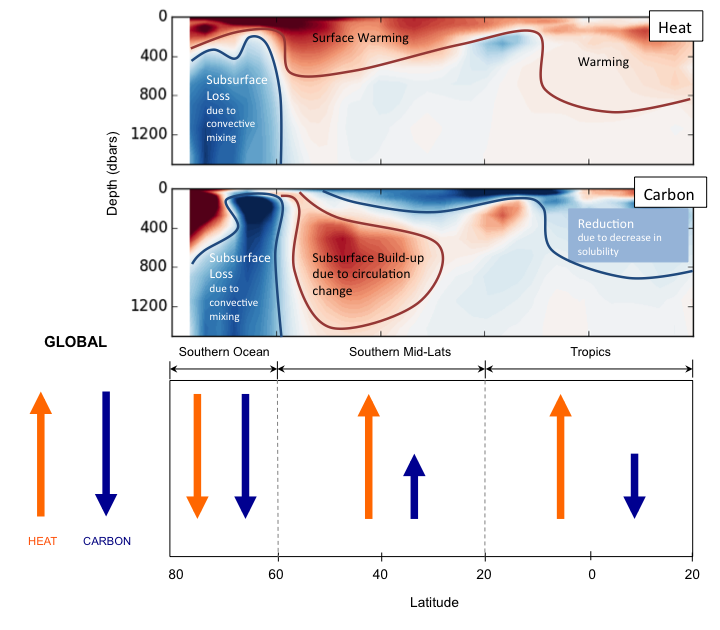
\includegraphics[width=1\linewidth]{schematic.png}
\caption{Schematic summarizing regional variability in oceanic heat and carbon
during a convective year. Arrows designate the sense of global and regional
inventory change during a convective year, positive indicating an increase in
oceanic content.}
\label{fig:schematic}
\end{figure}

The sub-surface variability structure is also depicted in Figure~\ref{fig:schematic}
and highlights the differences between heat and carbon.
During convection, both quantities decrease in the subsurface Southern Ocean.
Additionally, both heat and carbon show increases in the southern mid-latitudes,
but the temperature increases are contained in the surface, while DIC increases
at depth. This increase in subsurface DIC is likely a result of decreased
ventilation. Finally, the southern mid-latitudes and tropics show an increase in
surface temperature and a decrease in surface DIC. The variability in DIC here
is due to solubility decreases as a result of the temperature increase.

Comparing the magnitude of the modeled natural variability to the size of recent
observed trends can provide information on how detectible anthropogenic trends
are \citep{Thomas2015}. For the control simulations, the magnitude of global
carbon variability is about $\pm$ 3 PgC. This accounts for only approximately
3\% of the estimated anthropogenic uptake of carbon over the past few decades
\citep{Khatiwala2012,Sabine2004,Waugh2006}. The variability in global heat
content on the other hand is about $\pm$ 3 $\times 10^{22}$ J. This is a much
larger percentage (20\%) of the estimated uptake of anthropogenic heat in recent
decades \citep{Levitus2009}. These results suggest that changes in carbon
content due to anthropogenic activity are unlikely to be obscured by
long-timescale variability, but changes in heat content could be obscured. This
large natural variability in global heat content could explain why there is less
CMIP5 model agreement in oceanic heat uptake than there is for carbon uptake
\citep{Frolicher2009}.

If we assume these results hold for the real ocean, we would expect that during
the current non-convective period we would experience a subsurface warming in the Southern
Ocean and a slowdown of the intermediate water ventilation. Both these processes
have been documented in observational studies \citep{Purkey2012,Waugh2013b}, but
it is important to note that these changes could also be due to anthropogenic influences
such as greenhouse gas warming and ozone depletion in addition to variability in
WS convection.
The frequency of modeled WS convection is a hard to compare to real-life WS
convection because of the lack of an observational record in the Southern Ocean.
Additionally, \citet{DeLavergne2014a}
have shown that models that have frequent convection in preindustrial control
simulations have a significant reduction in convection under global warming
scenarios. This suggests that we may not observe another strong WS convective event,
and makes it extremely difficult to determine what frequency of WS convection is
`correct'.

The results of this study suggest that the atmosphere could exhibit significant
changes in temperature and CO$_2$ concentration in response to Southern Ocean
convective variability. A previous study by \citet{Cabre} using our
control version of the ESM2Mc model shows an increase in SH and global atmospheric
temperatures. This is because the additional flux of heat into the ocean is more
than balanced (and indeed is driven) by a decrease in clouds and ice, resulting
in an additional 0.15 PW of additional shortwave heating of the Southern Hemisphere
when convection is at its peak. An interesting extension of this
study would be to examine whether relatively small preindustrial changes in
atmospheric carbon dioxide could be associated with changes in SH temperatures,
as well as a more comprehensive examination of this process in Earth System
Models with variable atmospheric carbon dioxide.

A caveat with this study is that only a single model has been used. More
analysis should be conducted with additional model simulations to examine if
this relationship and the relative magnitudes of variability between heat and
carbon are consistent. Similar analysis with additional models could help to
understand the
intermodel spread of oceanic carbon content, and the larger intermodel spread
in  oceanic heat content \citep{Frolicher2014}, and also provide a better context
in which to analyze recent observational trends. Additionally, the model used in
this analysis has a relatively coarse resolution and parameterizations for
mesoscale eddies. \citet{Dufour2017} assessed the impact that model resolution has on
WS convection and concluded that horizontal model resolution has
an important impact on vertical stratification and the subsurface heat reservoir build-up.
However, the impact of resolution is not straightforward - a 1/4 degree ocean
behaved more like our high eddy diffusion model with relatively constant convection
while a 1/10 degree ocean model showed more stratification and behaved more
like our control model.
\citet{GRIFFIES2015} have additionally examined the impact eddies have on Southern
Ocean heat uptake and transport in eddy-permitting models
and have concluded that uncertain model
parameterizations tend to lead to model drift and less accurate lateral and
vertical heat distribution. These impacts need to be kept in mind when discussing
model simulations with parameterized eddies.



%\bibliography{/RESEARCH/library}
%%% Local Variables:
%%% mode: latex
%%% TeX-master: "thesis"
%%% End:

\graphicspath{{figures/chapter-oxygen/}}
% Specifies the directory where pictures are stored

\chapter{Relationship between age and oxygen}
\label{cha:oxygen}

\section{Introduction}
Characterizing the ventilation of the ocean interior is a fundamental goal of
oceanography. In order to do so, signatures of biological activity and transient
(i.e. a tracer with time-varying sources or sinks) tracers such as Chlorofluorocarbons
(CFCs) are used in to infer ventilation. The goal of this work is to evaluate
what we can learn from measurements of transient tracers and oxygen that have been
made in recent decades, focusing on the relationship between oxygen utilization
and water age inferred from transient tracers.

When examining the relationship between age and oxygen, it is generally assumed
that the two follow a negative relationship. Oxygen concentration is set at the
surface and generally decreases in the ocean interior due to biological
consumption. Age on the other hand, is set to zero at the surface and increases
in the ocean interior, characterizing the time spent since last in contact with
the surface. This relationship between age and oxygen is exploited in the
oceanography in two ways. The first is that allows for the indirect measurement
of the oxygen utilization rate to diagnose changes in ocean productivity, and
the second is that it allows for the possibility to use oxygen as a proxy for
age when examining changes in ocean circulation.

The primary sink of oxygen is the utilization by biology. For this reason, the
oxygen utilization rate (OUR) is a powerful tool for understanding ocean biology
and biogeochemistry. In the ocean interior, the OUR is generally very small and
therefore very difficult to directly measure. A commonly used solution to this is
to estimate the OUR as the derivative of the change in Apparent Oxygen Utilization
(AOU) over the change in age:

\begin{equation}
  OUR = \frac{dAOU}{d\Gamma} = \frac{d([O_{2 sat}] - [O_2])}{d\Gamma}
\end{equation}

This definition of OUR is fairly ubiquitous in the ocean biogeochemistry
community. It is referenced in multiple textbooks~\citep{Sarmiento2006,Emerson2008},
and has been used extensively in the literature to draw conclusions on organic
matter transport from the surface ocean to the deep~\citep{Jenkins}, and quantify
biological productivity in the ocean~\citep{Burd2010}. However, as discussed
in~\citet{Koeve2016}, this method for determining OUR assumes that the advective
and diffusive transports impact the age and oxygen in the same way. This will
only be strictly true if the two tracer fields have the same distribution of
internal sinks, something which in general is not the case. The authors found
that when averaged over three coupled physical and biogeochemical ocean models,
the OUR determined by this method underestimated the actual modeled OUR by a
factor of 3. This result suggests that the relationship between age and oxygen
is not as straightforward as often assumed.

Another way that oxygen and age have been combined in the field is through the
suggestion that oxygen could be used as a proxy for age for quantifying changes
in ocean circulation. While transient tracers are a useful tool for understanding
ocean circulation, there are some well-documented complications in estimating age
from such tracers~\citep{Haine2002}. Additionally, transient tracer
measurements are made much less frequently than oxygen measurements, making it
impossible to directly estimate ocean age from the historical record. To resolve
these problems, the possibility of exploiting the age-oxygen relationship and
using oxygen as a proxy for age has been suggested in the physical oceanography
community. Changes in oxygen concentration could be used to diagnose changes in
ocean circulation when age measurements are unavailable~\citep{Deutsch2005,Kwon2016}.
Similarly, \citet{Brennan2008} use AOU to improve the detectability of anthropogenic
changes in overturning in a climate model. However, in order for these methodologies
to be successful, the negative correlation relationship between age and oxygen
(or positive correlation relationship between age and AOU) would need to be robust
over time and space.

In this chapter, we evaluate the relationship between age and oxygen to shed
light on where it may be valid to use oxygen as a proxy for age and to consider
the use of defining OUR as AOU divided by mean age. Because it crosses the western
boundary current in the North Atlantic Ocean, and has measured both transient
tracer and oxygen concentrations, Line W provides a unique opportunity to
investigate the assumed negative relationship between age and oxygen and examine
the robustness of the two mentioned applications of this age-oxygen relationship.
Because of the limited temporal resolution and spatial coverage of the Line W
observational data, we seek to put the observational data in context by performing
a similar analysis of an earth system model, GFDL ESM2Mc.

In the next section we introduce the Line W observational data set, describe how
transient tracer ages were derived, and discuss the earth system model specifications.
In Section~\ref{section:results} we explore the age-oxygen relationship in the observations and model,
and discuss mechanisms driving the resulting relationship. Finally, in Section~\ref{section:conclusions}
we share our conclusions.

% METHODS


\section{Methods}
\label{section:methods}
\subsection{Line W Observational Data}
\subsubsection{Data Collection}
The observational data set used in this analysis comes from the Woods Hole Oceanographic
Institute's (WHOI) Line W ship-based repeat hydrography study~\citep{Andres2017}.
Observations include full-depth temperature and salinity profiles, horizontal
velocity profiles from lowered ADCPs (LADCPs), and bottle-sampled transient tracer
and oxygen concentrations.  Data was collected once or twice-per-year (one cruise
in the spring and one in the fall) over the 2003-2012 period. The Line W cruise
line extends from just south of the coast of Cape Cod (40.29 N, 70.21 W) and
extends to Bermuda (32.16 N, 65.23 W - Figure~\ref{fig:observational_linew_model_interpolation}
(a)). The water property and velocity measurements were taken at 26 fixed sites
along Line W. The stations are more densely situated across the continental shelf
to resolve the Deep Western Boundary Current. The station spacing becomes greater
and temporal sampling frequency is lower along the end of the Line W tract, near Bermuda.

Temperature and salinity data was collected using a conductivity-temperature-depth
(CTD) instrument mounted on a rosette frame. Salinity (i.e. conductivity)
measurements were then validated with bottle measurements of salinity~\citep{Millard1930}.
Bottle measurements were sampled using 10-L Nisken bottles
mounted on a rosette. Generally, 23 bottle samples at various depths were taken
at each location along the cruise line. Water samples were analyzed on board for
salts, dissolved oxygen, and transient tracer concentrations. The transient tracers
sampled include multiple chlorofluorocarbon compounds: CCl$_3$F (CFC-11), CCl$_2$F$_2$ (CFC-12),
and CClF$_3$ (CFC-13).

The data is available on the WHOI Line W website (http://www.whoi.edu/science/PO/linew).

\begin{figure}
\centering
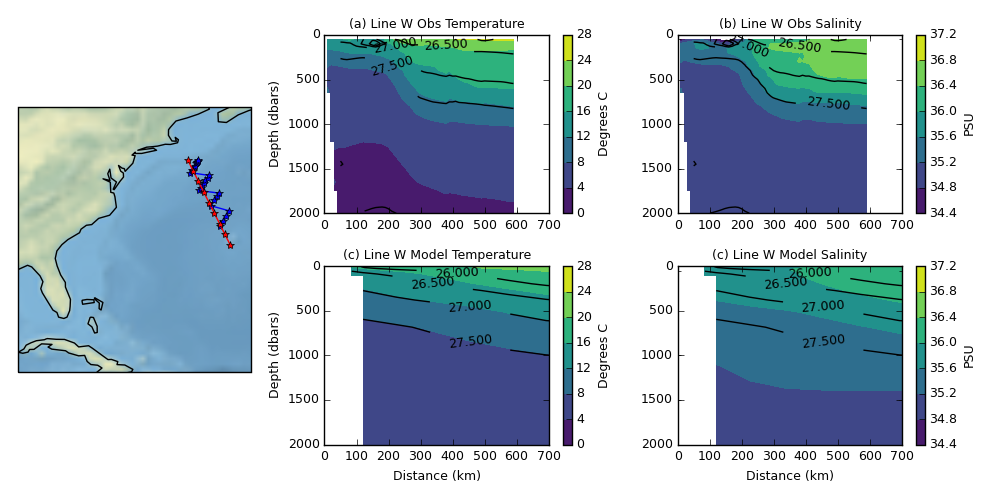
\includegraphics[width=\linewidth]{linew_interpolation.png}
\caption{Observational Line W and model interpolation. (a) and (b) climatologies of observational temperature and salinity. (c) and (d) Line W interpolated model temperature and salinity.}
\label{fig:observational_linew_model_interpolation}
\end{figure}

\subsubsection{Data Processing}
For purposes of visualization and comparison with the Earth System Model, the
data has been interpolated to a grid with a vertical resolution of 100 dbars and
horizontal resolution of 10 km. Cross-sections of oxygen concentration and mean
age (described below) for two years are shown in Figure~\ref{fig:obs_age_oxygen}.
Oxygen is generally high at the surface and decreases with depth, reaching a
minimum between depths 250 dbars and 750 dbars. Age on the other hand is at a
minimum at the surface and increases with depth. Figure~\ref{fig:obs_age_oxygen}
additionally shows the time-series of two locations along Line W (as indicated
by the black boxes). The first time-series (Figure~\ref{fig:obs_age_oxygen} (e))
suggests that there is a positive correlation between age and oxygen. The second
time-series (Figure~\ref{fig:obs_age_oxygen} (f)) on the other-hand shows the
anticipated negative relationship between age and oxygen.

Because temperature and salinity impact oxygen saturation, we additionally
compute the Apparent Oxygen Utilization for the observational data:

\begin{equation}
AOU = O_{2 sat} - O_2
\end{equation}

where $O_{2 sat}$ is the equilibrium saturation concentration of oxygen,
calculated as a function of temperature and salinity, and $O_2$ is the observed
oxygen concentration. The AOU is a measure of how under-saturated the oxygen sample
is. Using the AOU instead of oxygen concentration allows us to ignore the impacts
of temperature on the oxygen measurement.


\begin{figure}
\centering
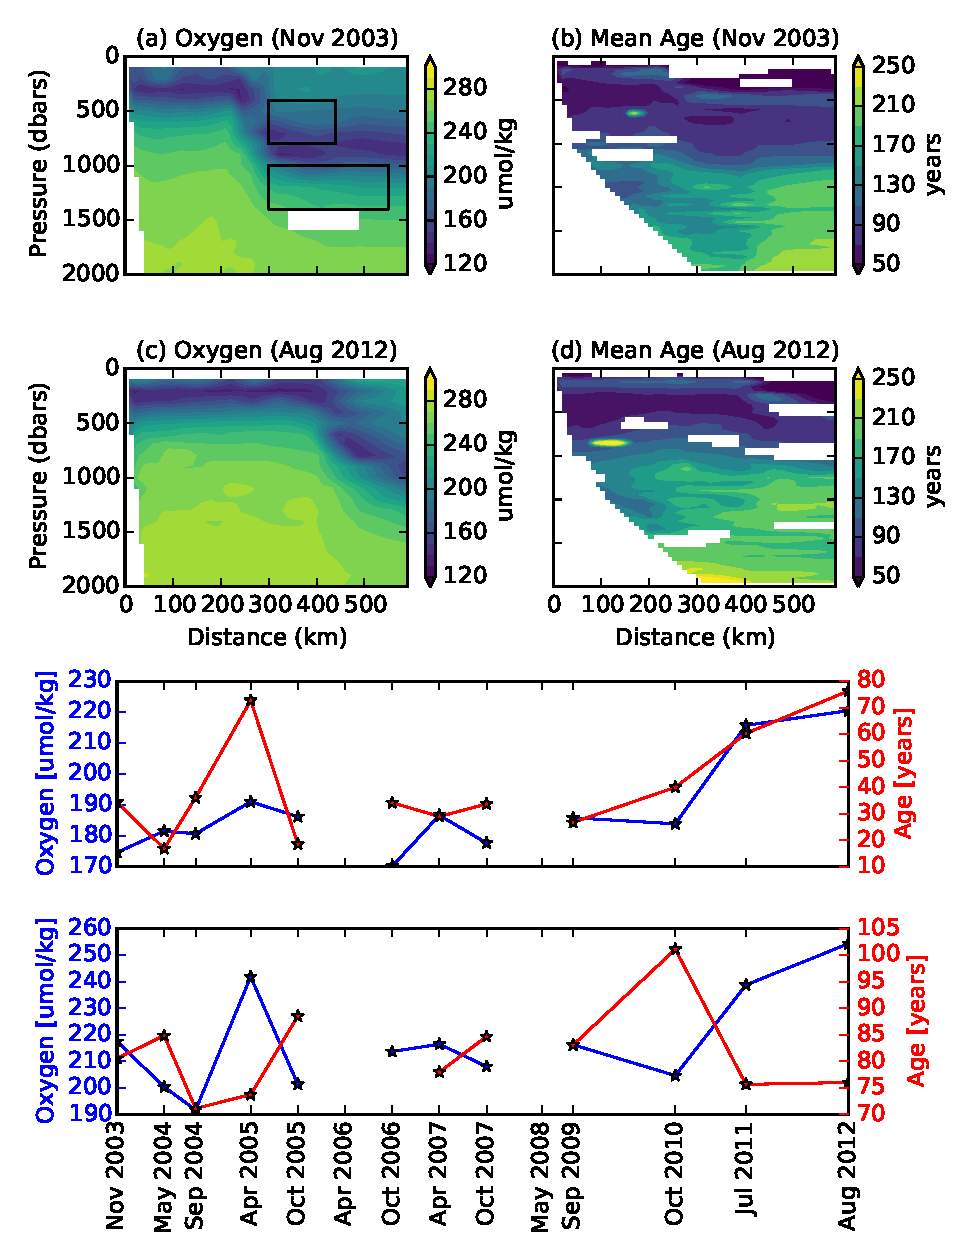
\includegraphics[width=\linewidth]{age_oxygen_ts.pdf}
\caption{Observational age and oxygen for two years. Subplots (a) and (b) show observational oxygen and
age from November 2003 while (c) and (d) show the oxygen and age from August 2012.
(e) and (f) show the timeseries of oxygen (blue) and age (red) averaged over the
boxes shown in subplot (a).}
\label{fig:obs_age_oxygen}
\end{figure}

\subsubsection{Mean Age Calculation}
A critical component to understanding ocean circulation and quantifying biological respiration is estimating the age of the water - or how long since the water was last in contact with the surface. Doing this with observations is not easy, but transient tracers make it possible. Because of the atmospheric time history of Chloroflourocarbons (CFCs), and the fact that CFCs have no sources and sinks in the ocean, CFCs are often used to quantify the age of ocean water. The simplest way of doing this is to assume that CFCs are in equilibrium with the atmosphere when they leave the ocean surface and are then transported advectively to the observation site. One can then deduce the date at which the water was subducted by matching the partial pressure of CFCs in the water to the date at which they had that concentration in the atmosphere.  This assumes that the transport to a given point can be characterized by a single timescale- the advective time.
In reality, estimating the age is complicated by mixing in the ocean. Because all flow is a combination of advective and diffusive flow, there is no one timescale that characterizes the time that a parcel of water has taken to reach an interior location from the surface. Because of this advective and diffusive flow, we characterize the timescales of a given point in the ocean interior with a distribution if transit times (or transit time distribution).
	The basis for this transit time distribution (TTD) approach for estimating ocean age is that for steady transport, the interior concentration of a transient tracer, $c(r,t)$, is given by (Haine and Hall, 2002):

\begin{equation}
	c(r,t) = \int_{0}^{\infty}c(t-t')G(r,t')dt'
\end{equation}

where $G(r,t)$ is a function describing the TTD at location r and time t. Measurements of CFC-12 were used to estimate the TTD assuming that (1) the TTD follows an Inverse Gaussian distribution and (2) the ratio of the mean width to mean age ($\Delta⁄\Gamma$) of the Inverse Gaussian is approximately equal to 1 (Waugh et al, 2003; Waugh et al, 2004; Waugh et al, 2006). Making the assumptions in order to estimate $G(r,t)$ using the Line W CFC-12 data and using the atmospheric history of CFC-12 allows us to estimate the mean age of the water sample.

\subsection{Model Simulation}
In addition to the observational data, we use an Earth system model (GFDL ESM2Mc)
to quantify the relationship between oxygen and age. GFDL ESM2Mc~\citep{Galbraith2011}
is a coarse resolution configuration of the GFDL ESM2M~\citep{Dunne2012}. The model
has an atmospheric resolution of 3.875$^{\circ}$ $\times$ 3$^{\circ}$  with 24 vertical levels. The ocean
model is non-Boussinesq, using pressure as the vertical coordinate, and has a
resolution of 3$^{\circ}$ $\times$ 1.5$^{\circ}$  and 28 vertical levels. The oceanic model also has a
coupled biogeochemical module referred to as the Biogeochemistry with Light Iron
Nutrients and Gases (BLING) model~\citep{Galbraith2010}. Although this module
uses a highly parameterized biological cycle, it predicts patterns of carbon and
oxygen change in response to global warming that are very similar to a more
complex biogeochemistry simulation in ESM2M~\citep{Small2014}. The model
also computes an ideal age~\citep{Thiele1990}, setting this tracer to
zero in the surface box and allowing it to increase at 1 yr/yr in the ocean
interior. For a full description of the model simulation, reference Section 3.2.1.

The model is interpolated to 1 $\times$ 1  grid in the North Atlantic and then
interpolated to a line extending from position (40$^{\circ}$N, 69$^{\circ}$W)
to (22$^{\circ}$N, 60$^{\circ}$W) to match observational Line W
(Figure~\ref{fig:observational_linew_model_interpolation} (a)). The model shows
a similar temperature and salinity profile on Line W compared with the
observations (Figure~\ref{fig:observational_linew_model_interpolation} (b) - (e)).
The model simulation is used to help put the observational analysis in in spatial
context and to investigate potential mechanisms affecting the age-oxygen relationship.

\begin{figure}
\centering
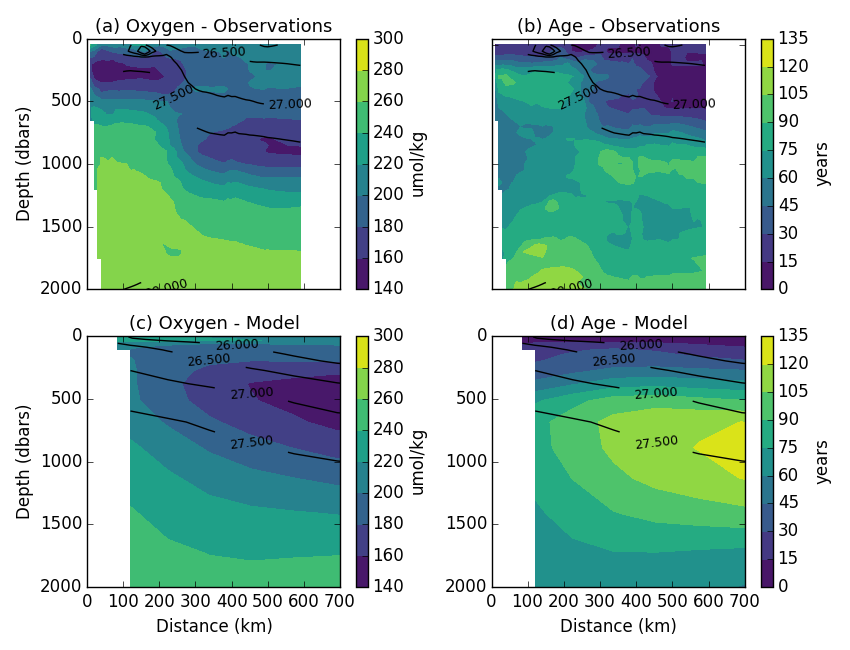
\includegraphics[width=\linewidth]{age_oxygen_climatology.png}
\caption{(a) Oxygen climatology and (b) age climatology from observations along Line W.
Contour lines show average neutral density. (c) Oxygen climatology and (d) age
climatology from the model simulation. Contour lines show the average netural density.}
\label{fig:oxygen_age_climatology}
\end{figure}

%%%%%%%%%%%%%%%%%%%%%%%%%%%%%%%%%%%%%%%%%%%%%%%%%%%%%%%%%%%%%%%%%%%%%%%%%%%%%%%%
% RESULTS
%%%%%%%%%%%%%%%%%%%%%%%%%%%%%%%%%%%%%%%%%%%%%%%%%%%%%%%%%%%%%%%%%%%%%%%%%%%%%%%%
%% Section 1
\section{Results}
\label{section:results}
\subsection{Age and Oxygen Relationship}

The climatologies of the calculated mean tracer age and oxygen concentration from
the Line W observations are shown in Figure~\ref{fig:oxygen_age_climatology} (a)
and (b). As expected, on large spatial scales there appears to be a negative relationship between the age and oxygen.
There is relatively high oxygen concentration and zero age at the surface, consistent
with the surface waters being in contact with the atmosphere, resulting in
near-equilibrium in oxygen and CFC concentrations. Age then generally increases
with depth, reaching a local maximum at just below the average depth of the 27.5
neutral density surface. Oxygen on the other hand generally decreases with depth,
reaching a local-minimum along the average depth of the 27.5 neutral density surface.
The spatial patterns of age and oxygen generally point towards a negative relationship
between the two qualities, particularly at intermediate depths. Oxygen shows a
core of minimum values with two intense patches, where the concentrations drop
below 160$\mu$mol kg$^{-1}$, on either side of the Gulf Stream more or less aligned
with the 27.5 neutral density surface. Age also shows two such patches of high
values on either side of the Gulf Stream at similar depths. However, there are
interesting differences in the detailed structure. First, the age maximum just
below the ventilated thermocline at distances 300-500 km offshore occurs at a depth of 1000
dbars. This is lower in the water column than the oxygen minimum, which occurs
at an approximate depth of 800 dbars. Additionally, there is significantly more
spatial variability in the age in the deeper regions across all distances than
is seen in the oxygen climatology. These differences between the spatial patterns
suggest the relationship between age and oxygen is likely more complicated than has
been suggested in previous work.

As discussed in the introduction, we also examine the age-oxygen relationship in
an Earth System Model. The vertical structure of the modeled oxygen and age
climatologies (Figure~\ref{fig:oxygen_age_climatology} (c) and (d)) are similar
to the observed climatologies, though somewhat offset in density space. The
modeled oxygen concentration exhibits a local minimum close to the 27.0 average
neutral density surfaces, while the age reaches a local maximum on the 27.5
average neutral density surface. While the vertical structure of age and oxygen
in the model are similar to the observations, there is a more obvious offset
between the depths of the local oxygen minimum and local age maximum in the model.
As with the observational data, this suggests a possible breakdown of the suggested
negative relationship between age and oxygen in this region. Note also that our
relatively coarse model does not allow for separation of two cores of low oxygen
water by the Gulf Stream-only the offshore core seen in the observations
is simulated with some measure of fidelity.

To better quantify the temporal relationship between mean age and oxygen, the
Pearson correlation coefficient between age and oxygen is calculated for
locations along Line W (Figure~\ref{fig:correlations} (a)).  Although this figure shows the anticipated
negative correlation between age and oxygen, in much of the plot the correlations
are relatively low.  Moreover, two regions of positive correlation are apparent
between 200 and 400 km offshore. One positive correlation region is at approximate
depths 500-750 dbars (between neutral density surfaces 27.0 and 27.5), and the
second is slightly deeper at depths 1250 - 2000 dbars.

One possible reason for the lack of a tight relationship between oxygen and age
is that oxygen concentration depends on solubility and thus on temperature and
salinity. In order to correct for this effect, we also examine the relationship
between the age and AOU. The AOU is a measure of how under-saturated the oxygen
concentration is. This under-saturation is usually due to the biological
consumption of oxygen but may also see an effect from incomplete equilibration
of sinking source waters, particularly in convective regions. Analyzing the
relationship between AOU and age gives us similar information to the age-oxygen
relationship, however, because we are subtracting the oxygen concentration from
the oxygen saturation, the AOU-age relationship will be the opposite sign
(mainly positive) and the AOU-age relationship removes the impacts of temperature
(and salinity) on oxygen saturation.

The Pearson correlation coefficient between age and AOU
(Figure~\ref{fig:correlations} (b)) shows a positive relationship between the
two quantities.  Similar to the pattern seen in the age-oxygen correlation
coefficients (Figure~\ref{fig:correlations} (a)), there are two regions with
anomalous correlation. One upper region of near-zero correlation, corresponds
with the upper region of positive correlation seen in Figure~\ref{fig:correlations}
(a). This suggests that this positive correlation between age and oxygen in this
region largely results from temperature effects. Younger waters in this region
are colder and thus hold more oxygen-countering any impacts from less
remineralization. Note however, that even with temperature effects removed the
AOU-age correlation remains low. Moreover, the region with anomalous O2-age
correlation in the deeper waters also shows an anomalous AOU-age correlation
(negative).  The fact that these patterns exist in the age-AOU correlation pattern
in addition to the age-O2 correlation pattern suggest that we need to find a
mechanism other than solubility changes for explaining such variability.

\begin{figure}
\centering
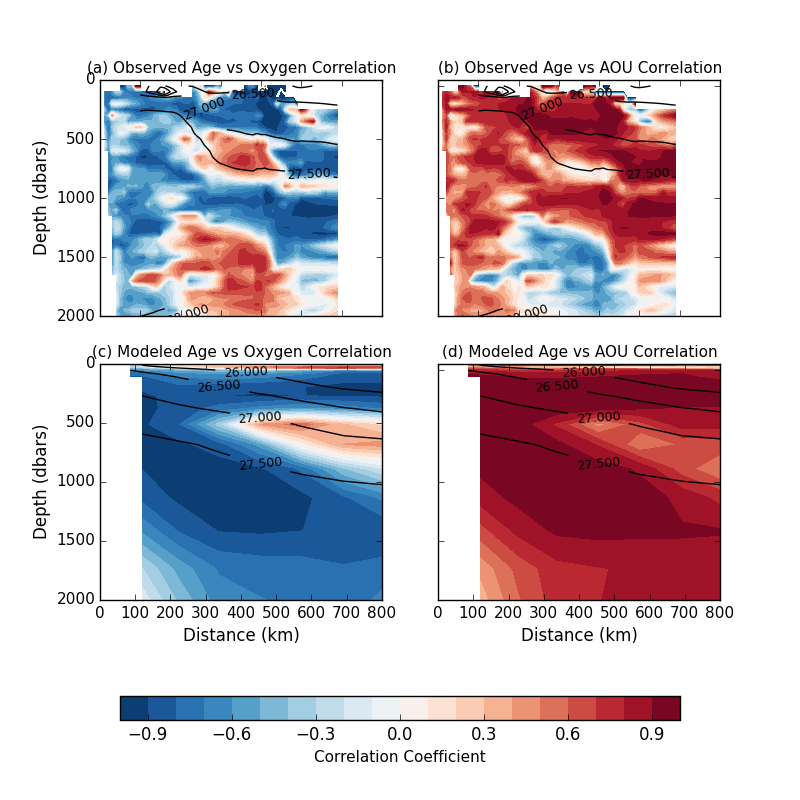
\includegraphics[width=\linewidth]{correlation.png}
\caption{Pearson correlation coefficients for age versus (left) oxygen and (right)
AOU for Line W observations. Contour lines indicate average neutral density climatology.}
\label{fig:correlations}
\end{figure}

We also show the Pearson correlation coefficient for the model simulation
(Figure~\ref{fig:correlations} (c) and (d)). Although the model also shows the
expected negative correlation between age and oxygen over much of the domain,
the correlation is far from uniform with one core of strong positive correlation
in denser waters around 1000 dbars and a second layer of negative correlation at
around 300 dbars.  As in the observations, there is a region of positive correlation
(with correlation coefficient of approximately 0.4) between the negative correlation
layers, starting at distance 400 km and extending to the end of Line W. This region
of positive correlation is similar to the upper region of positive correlation seen
in the observational record. Interestingly, in the model simulation, there is no
deeper region of positive correlation as seen in the observational correlation,
although there is a decline in the correlations as one approaches the coast below
1500 dbars.

The modeled age-AOU temporal correlation shows a very consistent pattern with the
modeled age-oxygen correlation. The area of anomalous correlation (now negative)
around depth 500 dbars is greatly reduced in Figure~\ref{fig:correlations} (d),
suggesting that a fraction of the positive correlation seen in the age-oxygen
correlation is due to solubility- a signal similar to that seen in the observations.
However, as in the observations this region still has a reduced positive correlation,
suggesting some additional mechanism is impacting the age-AOU relationship.

\subsection{Age and Oxygen/AOU Scatterplots}

To better visualize and analyze the relationship between the mean age and oxygen
along observational Line W, we show the scatter plot of age versus oxygen in
Figure~\ref{fig:scatter_plots} (a). The scatter points are colored with each
location's temporal correlation coefficient (same as in Figure~\ref{fig:correlations}
(a)). The ``S-shape'' of the age-oxygen scatterplot relationship roughly follows
the depth of the water column, with the surface waters at the left end of the
``S-shape'' and the deep waters at the right end. The positive correlation regions
indicated from Figure 4 (a) also appear in this relationship.

The scatter plot relationship between age and AOU is also shown
(Figure~\ref{fig:scatter_plots} (b)).  Similar to the age-oxygen scatter plot,
the age-AOU scatter plot also roughly follows depth, with the surface waters at
the left-hand side of the scatter plot, transitioning to the deeper waters at
the right hand-side. The upper region of reduced/zero correlation discussed in
Figure~\ref{fig:correlations} (b) is seen on this diagram at an age of 50 years,
just before the maximum in AOU. Additionally, the deeper region of negative
correlation discussed in Figure 4 (b) is seen on this diagram on the almost-flat
tail end of the scatterplot. Visualizing the age-AOU relationship in this way is
a powerful tool because it allows us to gain initial insight to the mechanisms
governing the AOU variability. The dashed lines represent expected linear
relationships between age and AOU with the slope of the linear relationship being
directly proportional to the rate of remineralization. At the surface, where
sinking particulate matter has higher concentrations and is more easily decomposed,
we have increased rates of remineralization, and therefore we would expect the
age-AOU relationship to follow one of the linear relationships with a higher slope.
As we move deeper in the water column, the slopes should decrease to reflect the
slower rates of remineralization in the deep ocean.

If the variability in AOU were driven exclusively by changes in the rate of
ventilation (but not the pathways of ventilation or the rate of remineralization),
we would expect the age-AOU relationship to fall along one of the dashed lines.
The upper region does follow this linear relationship (with a slope of
1.7$\mu$mol yr$^{-1}$). When the age-AOU relationship does not follow these linear
lines however, it indicates that other processes are influencing the spatial
(and thus potentially the temporal) variability in AOU. The right-hand tail of
this relationship, where the correlation is negative, does not follow the
anticipated linear relationship, and therefore we can infer that some additional
process is influencing the AOU-age relationship. This region is also one where
the correlation between AOU and age is (unexpectedly) negative.

The shape of the modeled relationship between age and oxygen is similar to the
shape of the observed age-oxygen relationship (Figure~\ref{fig:scatter_plots} (a)),
suggesting that the model captures the mean relationships to a surprising extent
(given the coarseness of its resolution and the simplicity of its biological model).
However, there are clear differences between the modelled and observed variability.
In the model, the area of positive correlation between the age and oxygen occurs
in the region of the oxygen minimum, which is a region where the age is still
increasing with depth. Since the shape of the relationship roughly follows depth,
movement along this curve would correspond to vertical movement in the water column.
In this region, if we move lower in the water column, age increases and oxygen also
increases, therefore resulting in a positive correlation. This suggests that vertical
movement in the water column could be causing the positive correlation. In the
observations, however, the upper region of positive correlation is found above the
oxygen minimum and the lower region is found around a weak age minimum. The
corresponding point on the modelled age-oxygen plot shows some near-zero correlations,
but no positive values.

\begin{figure}
\centering
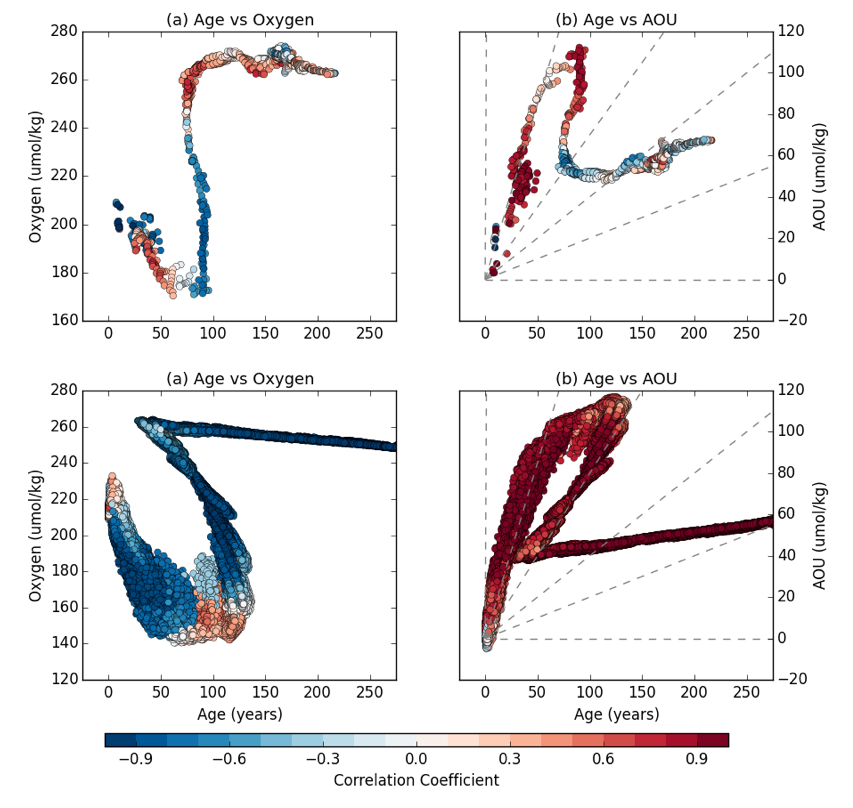
\includegraphics[width=\linewidth]{age_aou_scatter.png}
\caption{Scatter plot of age versus observed (a) oxygen and (b) AOU and
modeled (c) oxygen and (d) age for distances 300-400 km.
Colors indicate correlation coefficient of given relationship. Dashed grey lines indicate linear relationship between age and AOU.}
\label{fig:scatter_plots}
\end{figure}

The modeled age-AOU scatter plot (Figure~\ref{fig:scatter_plots} (d)) has
similarities to the observed age-AOU relationship (Figure~\ref{fig:scatter_plots}
(b)), but has a much more pronounced mid-depth age minimum. As in
Figure~\ref{fig:scatter_plots} (b), the dashed grey lines represent the linear
relationship between the age and AOU. In the upper region of the domain, the age
and AOU follow this linear relationship quite closely (with a slope of 1.7$\mu$mol yr$^{-1}$
- similar to the observations). Slightly deeper in the water column, the age and
AOU also closely follow a linear line, with a slightly smaller slope (slope of 0.8).
In the deeper waters however, the age-AOU relationships break away from the linear
model, suggesting additional processes impacting the AOU variability.

Some part of the mean relationship is driven by the well-known decrease in the
remineralization of organic material with depth~\citep{Armstrong2002,Klaas2002}
as unprotected organic materials are preferentially consumed near the surface.
This would move points between a steeply-sloped linear relationship near the
surface to lying along a line with a flatter slope at depth. An additional
factor is that the pathways of ventilation change with depth, with waters near
the deep age minima more affected by the southward flow of North Atlantic Deep
Water. These different factors have the potential to affect the variability as
well. In particular, changing pathways of ventilation would be expected to
change the mix of water masses seen at a given point. Assuming the water masses
involved in this mixing are reflected in the AOU-age structure, such changes
might be expected to produce relationships parallel to the age-AOU curve - which
in many locations would imply anti-correlation (where the mean curve slopes down
to the right) or near-zero correlation (where the mean curve is oriented either
horizontally or vertically). We note that when the age-AOU curve lies along one
of these dashed lines, it is impossible to distinguish changes in ventilation
rate from changes in water mass type without bringing in more information.

The region of reduced positive correlation seen in the depth profile of the age-AOU
Pearson correlation coefficient (Figure~\ref{fig:correlations} (d)) is seen in the
age-AOU scatterplot (Figure~\ref{fig:scatter_plots} (d)) at the apex of the scatter
plot, where the AOU goes from increasing with age to decreasing with age. This
region occurs between the two regions of strong linear relationship between age
and AOU as discussed above. This result suggests that it is a change in the
fraction of water associated with two water masses that is contributing to the
reduced positive correlation in age versus AOU (or positive in the age-oxygen
correlation).

This analysis provides some initial insight to why the age-oxygen relationship
displays an area of positive correlation. The age-AOU scatter plot suggests that
mixing between water masses may be contributing to the anomalous correlation in
the age-oxygen and age-AOU relationships. In the next section, we will investigate
the mechanisms driving the modeled variability in age and oxygen further,
examining whether the results can be simply explained in terms of vertical
excursions of density, or whether more subtle changes in circulation are involved.

\subsection{Mechanisms Driving Age and Oxygen Variability}
In this section, we will use the model simulation to assess the spatial extent of
the anomalous correlation outside of Line W and diagnose the most likely mechanisms
responsible for the break-down in the anticipated age-AOU relationship.

\subsubsection{Horizontal Extent of Anomalous Correlation}

To determine the horizontal extent of the anomalous correlation between age and
AOU, we show the age-AOU temporal correlation from the model on various neutral
density surfaces over the entire North Atlantic basin (see left-hand side of
Figure~\ref{fig:iso_correlations}). These correlations show that the temporal
relationship between age and AOU is largely positive throughout the entire domain
with Pearson correlation coefficients exceeding 0.6 in most of the basin. There
is a region at the end of Line W where the age-AOU correlation is reduced. This
is most prominently seen on the lower neutral density surfaces
(Figures~\ref{fig:iso_correlations} (e) and (g)).

The subplots on the right-hand side show the correlation on each designated
density surface ignoring the impacts of vertical heave in the isopycnals, while
the subplots on the left side do include vertical isopycnal heave as described
by the following equations:

\begin{equation}
	r_{\mathrm{with \; heave}} = \mathrm{corr}(\Gamma, O_2)|_{\gamma_n = 27.0}
\end{equation}

\begin{equation}
	r_{\mathrm{without \; heave}} = \mathrm{corr}(\Gamma|_{\gamma_n = 27.0}, O_2|_{\gamma_n = 27.0})
\end{equation}

In both equations (4.4) and (4.5) above, $\gamma_n$ designates the depth of a
neutral density surface and the overbar designates the time average. It is
important to distinguish between these two methods of neutral density interpolation
because the 'with heave' method includes the impact of vertical motion and allows
us to determine the extent that vertical motion impacts the correlation. The
positive correlation appears to be more significantly reduced on the neutral density
surfaces including vertical heave (left-hand side subplots). These results
suggest that the mechanism decoupling age and AOU is spatially limited to the
region at the end of Line W and includes some component of vertical mixing.

\begin{figure}
\centering
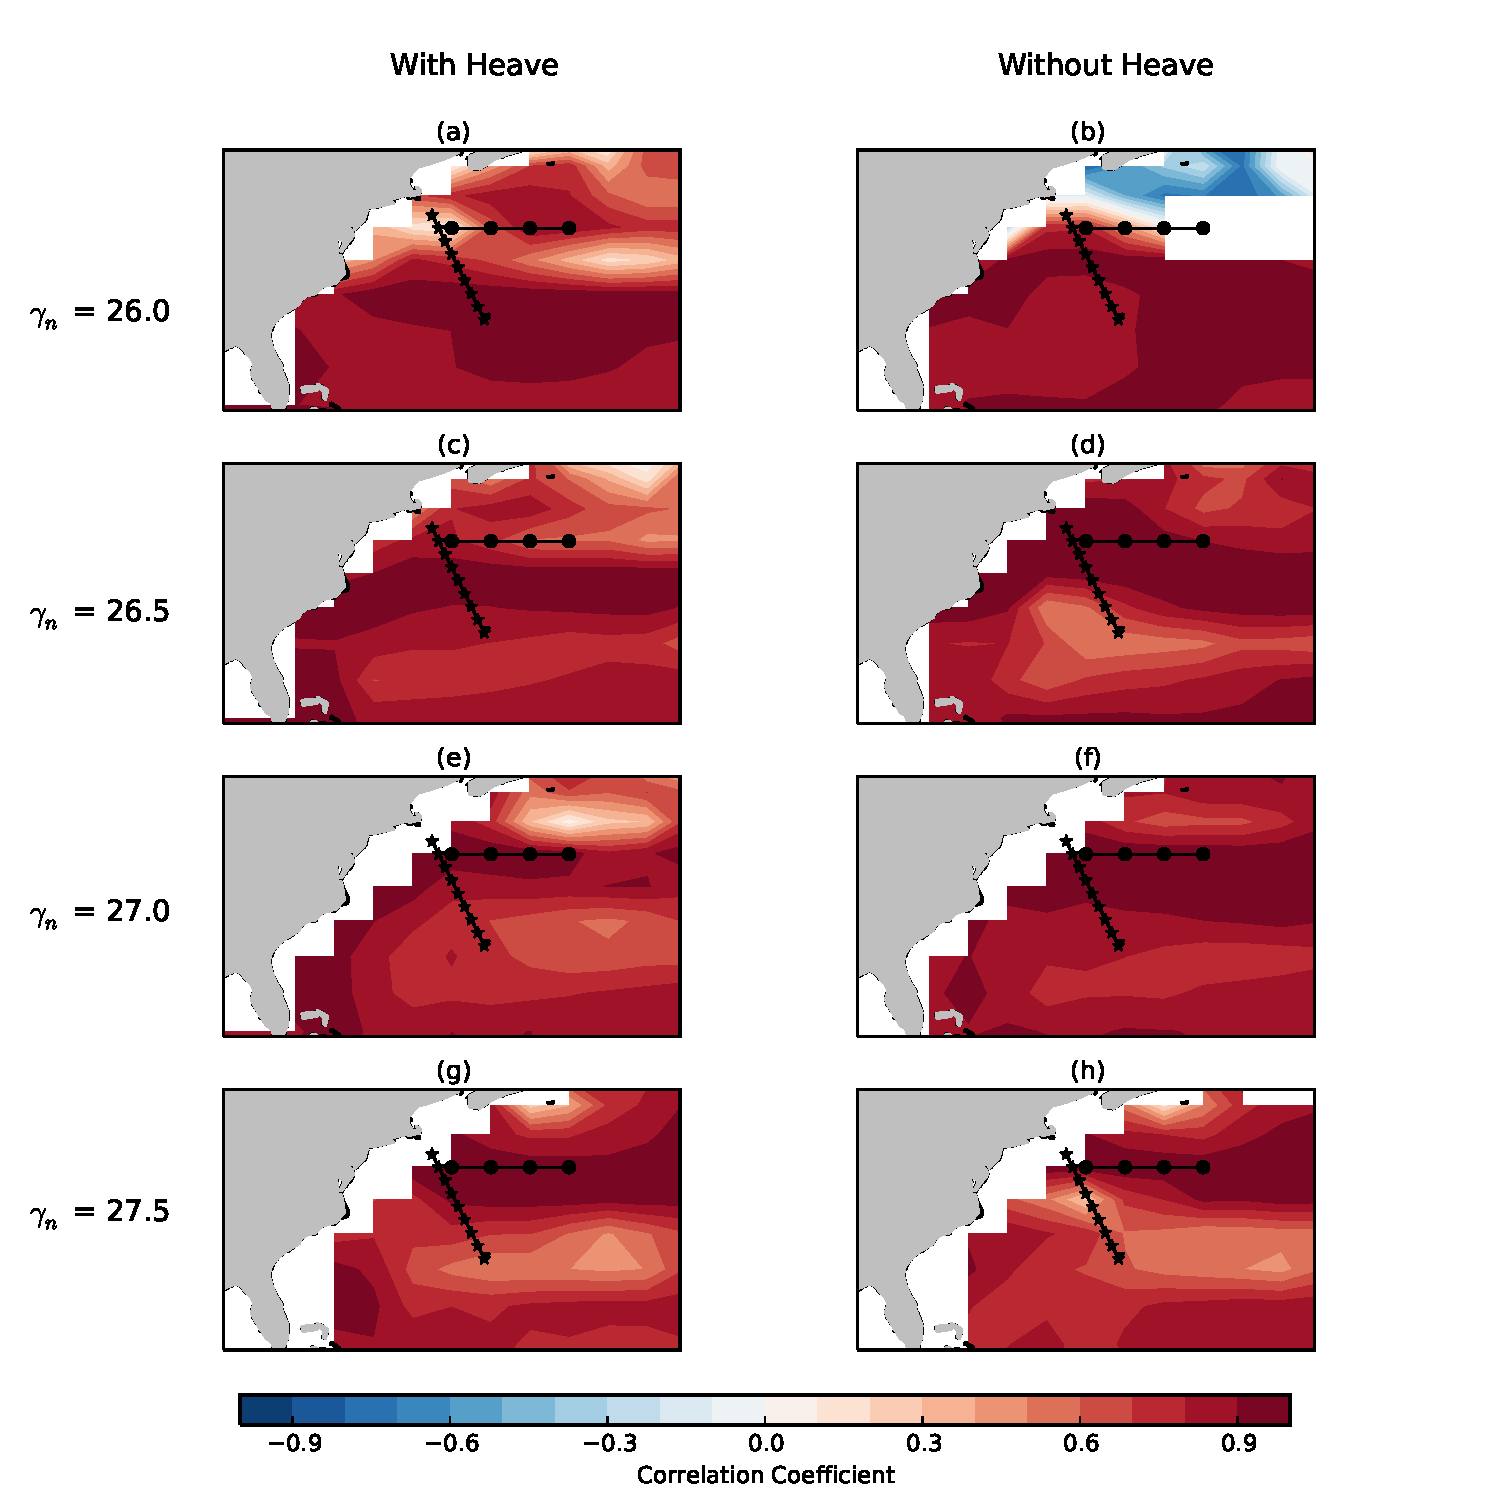
\includegraphics[width=\linewidth]{age_aou_corr_iso_sfc.pdf}
\caption{Correlation between age and AOU on various isopycnal surfaces. Left column indicate correlation calculated on average depth of the isopycnal surface, and therefore including contributions from isopycnal heave. Right column shows correlation calculated on the isopycnal surface and does not include contributions from heave.}
\label{fig:iso_correlations}
\end{figure}

\subsubsection{Line W versus Line 40N}
In order to diagnose what is causing this reduction in the negative age-oxygen
correlation and positive age-AOU correlation, we examine a region of the North
Atlantic where this breakdown of the age-AOU relationship does not occur and compare
it with Line W. We refer to this region as Line 40N, a hypothetical transect that
extends from Cape Cod eastward along latitude line 40 N. This hypothetical
transect follows along a region of the North Atlantic basin where the age-oxygen
correlation is strongly negative (not shown) and the age-AOU correlation is
strongly positive for all neutral density surfaces (Figure~\ref{fig:iso_correlations}).
Comparing Line 40N and Line W allows us to evaluate the differences between the
two and understand why Line W experiences these low correlations in the age-AOU
relationship.

One possible reason Line 40N maintains a strong positive correlation is due to
strong horizontal (primarily along-isopycnal) variability relative to Line W.
In order to diagnose the relative contributions of this along-isopycnal
variability and the isopycnal heave variability, we break the time rate of change
of age and AOU as follows:

\begin{figure}
\centering
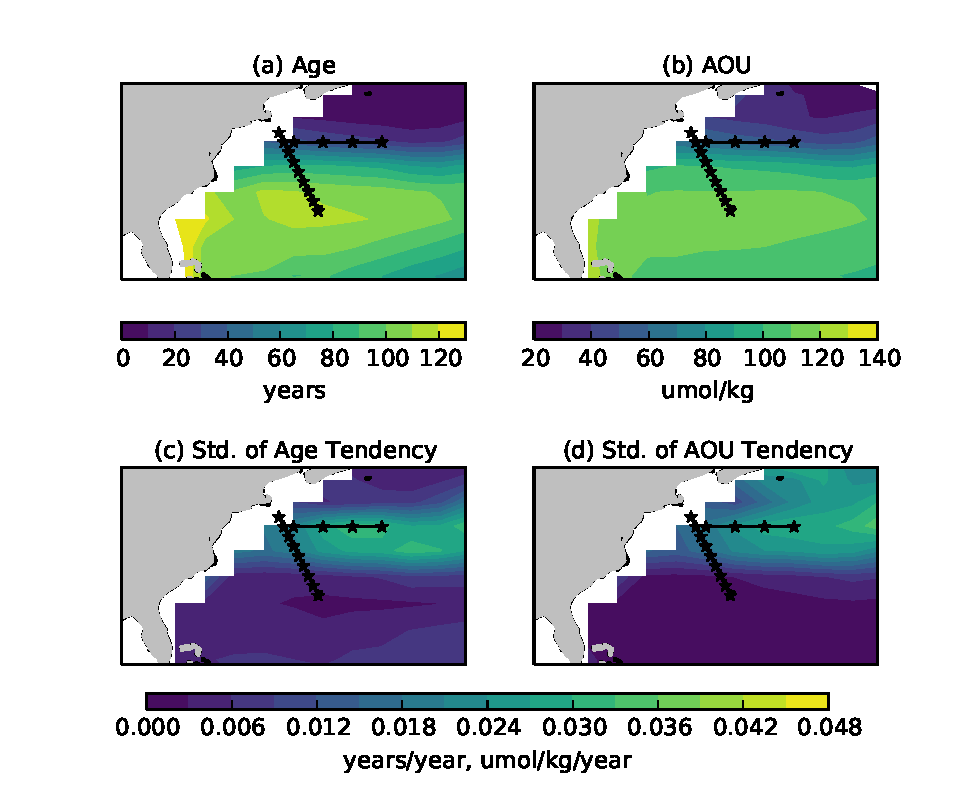
\includegraphics[width=\linewidth]{spice_figure.pdf}
\caption{Climatologies of (a) age and (b) AOU interpolated on neutral density surface 27.0. Bottom: Standard deviation of (c) age tendency and (d) AOU tendency interpolated on neutral density surface 27.0. Bottom plots are calculated as the standard deviation of the first term on right-hand side of equation (4).}
\label{fig:spice}
\end{figure}

\begin{equation}
	\left. \frac{\mathrm{d}\Gamma}{\mathrm{d}t}\right|_z = \left. \frac{\mathrm{d}\Gamma}{\mathrm{d}t}\right|_{\gamma_n=27.0} + \left. \frac{\mathrm{d}z}{\mathrm{d}t}\right|_{\gamma_n=27.0} \frac{\mathrm{d}\Gamma}{\mathrm{d}z}
\end{equation}

\begin{equation}
 \left. \frac{\mathrm{d}AOU}{\mathrm{d}t}\right|_z = \left. \frac{\mathrm{d}AOU}{\mathrm{d}t}\right|_{\gamma_n=27.0} + \left. \frac{\mathrm{d}z}{\mathrm{d}t}\right|_{\gamma_n=27.0} \frac{\mathrm{d}AOU}{\mathrm{d}z}
\end{equation}

\begin{figure}
\centering
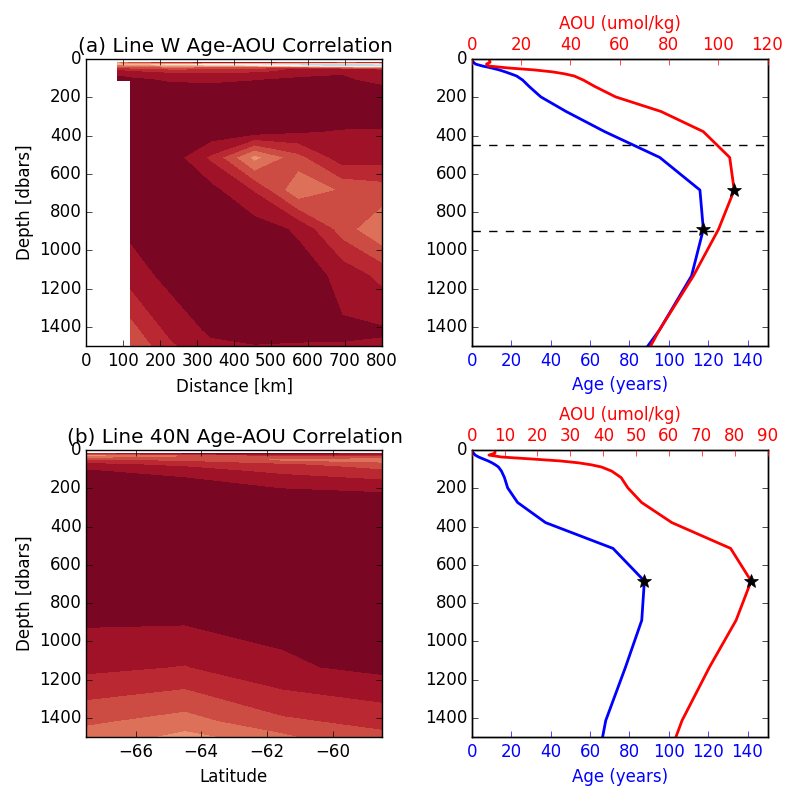
\includegraphics[width=\linewidth]{age_aou_corr_linew_line40N.png}
\caption{Age-AOU correlation and vertical profiles for (top) Line W and (bottom) Line 40N.}
\label{fig:vertical_profile}
\end{figure}

where the first term on the right-hand side refers to the age tendency on the
neutral density surface and the second term on the right-hand refers to the
contribution of vertical heave to the age variability. The climatologies of age
and oxygen on the $\gamma_n$=27.0 surface along with the standard deviation of the age
and oxygen tendencies along this surface are shown in Figure~\ref{fig:spice}.
The end of Line W, where the age-AOU correlation is near zero, lies in a
region where there is reduced horizontal gradient in age and oxygen. This is
significantly different to Line 40N, which lies in a region where the horizontal
gradients in age and oxygen (primarily in the meridional direction) are
particularly strong. This results in significantly more along-isopycnal variability
along Line 40N than Line W, as shown in figure~\ref{fig:spice} (c) and (d).
Because of the reduced along-isopycnal variability on Line W, the vertical heave
component (second term on right hand side of equations 4.6 and 4.6) may be important
in setting up the reduced positive correlation between age and AOU.

To investigate the vertical heave contribution to the age-AOU correlation, we show
the correlation between age and AOU for Line W and Line 40N in Figure~\ref{fig:vertical_profile}.
As previously discussed, Line W has an anomalous region of near-zero correlation.
Line 40N on the other hand has a strong positive correlation between age and AOU
in the upper 1500 dbars of the cross section. Figure 8 also compares the vertical
profiles of age and AOU along both lines. There is a visible offset between the
depths of the age and AOU maximum (as indicated by the stars) with the age
maximum occurring lower in the water column (900 dbars) than the AOU maximum
(700 dbars). Between the age and AOU maximums, age increases with depth and AOU
decreases with depth. It is between these depths that the reduced positive
correlation occurs between age and AOU (as indicated by dashed lines in
Figure~\ref{fig:vertical_profile}). We propose that the reduced correlation occurs
because of vertical motion acting on this particular vertical gradient in age and
AOU. When comparing the vertical profiles on Line W with Line 40N, we see that
there is no offset between the age and AOU maximums on Line 40N. We also examined
the magnitude of the vertical motion of the isopycnal surfaces (not shown) and
found no significant difference between Line W and Line 40N. While both transects
have similar levels vertical motion, the presence of a depth offset between the age
and AOU maximum in addition to decreased along-isopycnal variability result in
Line W having a reduced correlation between age and AOU.

Line W is unusual because the along-isopycnal (horizontal) gradients are so small
that variations in mixing or along-isopcynal velocity will have relatively small
impacts. This allows the vertical heave to dominate the local
variability in age and oxygen. Between depths 500 dbars - 750 dbars, this vertical
heave acts on an offset in the depths of the age maximum and oxygen minimum,
resulting in the observed positive correlation. In other regions of the basin
(Line 40N), the horizontal variation in transport is large enough to dominate the local variability.
Even though the same vertical heave and age maximum and oxygen minimum depth
offset is seen in this region, the large magnitude of horizontal variability maintains
the expected age-oxygen relationship.


%%%%%%%%%%%%%%%%%%%%%%%%%%%%%%%%%%%%%%%%%%%%%%%%%%%%%%%%%%%%%%%%%%%%%%%%%%%%%%%%
% CONCLUSIONS
%%%%%%%%%%%%%%%%%%%%%%%%%%%%%%%%%%%%%%%%%%%%%%%%%%%%%%%%%%%%%%%%%%%%%%%%%%%%%%%%

\section{Conclusions}
\label{section:conclusions}

Our analysis of the Line W observations of age and oxygen show that there is a
much more complicated relationship between the two quantities than one would naively
expect. The commonly held expectation of a negative relationship between age and
oxygen breaks down along observational Line W due to two regions of positive correlation.
One region of positive correlation is seen within the ventilated thermocline and
the other is lower in the water column. The same upper region of positive correlation
is seen in an Earth System Model (GFDL ESM2Mc) representation of Line W. We
additionally remove the impacts of temperature on oxygen saturation, by looking
at the age correlation with AOU. The age-AOU correlation also shows anomalous
(zero to negative) correlation in the observational data set and model simulation.

\begin{figure}
\centering
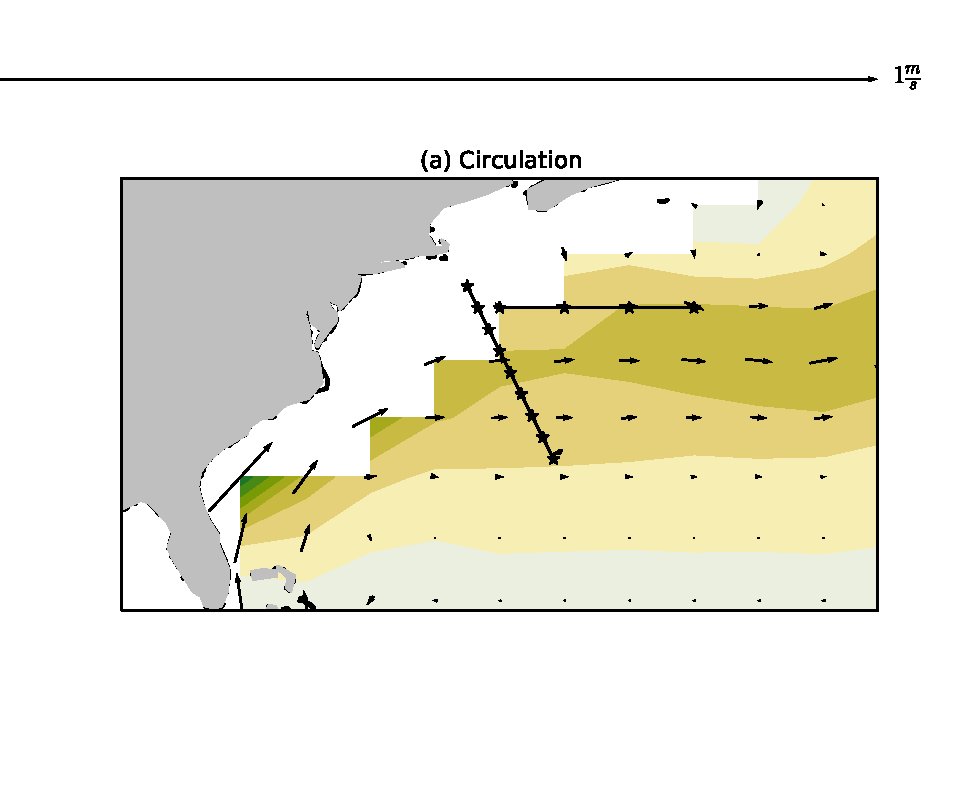
\includegraphics[width=\linewidth]{circulation.pdf}
\caption{Circulation on neutral density surface 27.0}
\label{fig:circulation}
\end{figure}

Our analysis of the Line W observations of age and AOU show that there is a much
more complicated relationship between the two quantities than one would naively
expect. The commonly held expectation of a positive relationship between age and
oxygen breaks down along observational Line W in two regions. One region of low
correlation is seen within the ventilated thermocline and the other is lower in
the water column. The same upper region of near-zero correlation is seen in an Earth
System Model (GFDL ESM2Mc) representation of Line W.

Because of the limited temporal resolution and spatial extent of the observational
data, we use the GFDL ESM2Mc to investigate the potential mechanisms causing the
anomalous correlation between and AOU. We show that the region of anomalous
correlation is limited to a region at the end of Line W, and to a few isopycnal
surfaces (surfaces 27.0-27.5). The end of Line W lies in a unique region in the
North Atlantic basin where the horizontal gradients in age and AOU are relatively
weak and thus the along-isopycnal variability is very small. Additionally, at the
bottom of the ventilated thermocline, there is a depth offset between the age
maximum and AOU maximum. Any vertical motion within this region, coupled with the
limited horizontal variability, would cause a break-down of the correlation between
the age and AOU.

The end of Line W is unique because it lies in the approximate center of the North
Atlantic gyre circulation (Figure~\ref{fig:circulation}). Because the horizontal
circulation in the middle of the gyre is very small, there is little horizontal
gradients in ocean tracers. In such regions, the balance between vertical heaving
of isopycnals (which acts to reduce age-AOU correlation) and horizontal mixing
(which mostly strengthens age-oxygen relationship) determines whether or not the
expected age-AOU relationship holds. Because of this delicate balance, one needs
to consider the local dynamics before assuming that oxygen and age follow a strong
negative relationship.



%\bibliography{/RESEARCH/library}
%%% Local Variables:
%%% mode: latex
%%% TeX-master: "thesis"
%%% End:

\chapter{Conclusions}
\label{cha:conclusions}

\section{Summary of results}

The main findings of this thesis are summarised as follows:
%\begin{enumerate}

\section{Limitations and further investigations}



%%% Local Variables:
%%% mode: latex
%%% TeX-master: "thesis"
%%% End:


%now enable appendix numbering format and include any appendices
%\appendix
%\appendix{Appendix 1}

 Appendix here

%\nclude{appendix2}


\baselineskip=14pt plus4pt % as HA
%next line adds the Bibliography to the contents page
\addcontentsline{toc}{chapter}{Bibliography}
%\addcontentsline{toc}{chapter}{Curriculum Vitae}
%uncomment next line to change bibliography name to references
%\renewcommand{\bibname}{References}
\bibliography{/RESEARCH/library.bib}        %use a bibtex bibliography file refs.bib
%\bibliographystyle{plain}  %use the plain bibliography style
\begin{cv}
\addcontentsline{toc}{chapter}{Curriculum Vitae}

  \begin{centering}
    \Huge{Jordan Thomas}\\
    \normalsize{Born: May 4, 1990}\\
    \normalsize{Wichita, KS}\\
  \end{centering}
  \vspace{1cm}
  \noindent\Large{Education}\\
  \vspace{0.2cm}
  \noindent\rule{\textwidth}{0.4pt}
  \normalsize{
  \noindent \textbf{Johns Hopkins University} (August 2012 -- Present) \hfill Baltimore, MD\\
	\indent PhD in Earth and Planetary Science\\
	\indent Masters in Earth and Planetary Science\\
	\indent Dissertation: Investigating Natural Variability in the Climate System\\
  \noindent \textbf{Pennsylvania State University} (August 2008-- May 2012) \hfill University Park, PA\\
	\indent Bachelors of Science in Meteorology\\
	\indent Concentration in Atmospheric Sciences \\
  \noindent \textbf{University of Southampton} (January 2011 -- July 2011)\hfill Southampton, UK\\
	\indent Minor in Oceanography\\
  }

  \vspace{1cm}
  \noindent\Large{Publications}\\
  \vspace{0.2cm}
  \noindent\rule{\textwidth}{0.4pt}
  \normalsize{
  Thomas J. L., Waugh D. W., and Gnanadesikan A. (2018) ``Relationship between ocean heat\\
  \indent and carbon variability''. \textit{Journal of Climate}. 31. 1467--1482. \\
  Brune W. H., Baier B. C., Thomas J.L., Ren X., Cohen R. C., Pusede S. E., Browne E. C.,\\
  \indent Goldstein A. H., Gentner D. R., Keutsch F. N., Thornton J.A., Harrold S., Lopez-\\
  \indent Hilfiker F. D. and  Wennbergm P. O. (2016) ``Ozone production chemistry in the pres-\\
  \indent ence of urban plumes''. \textit{Faraday Discussions}. 189. 169--189. \\
  Thomas J. L., Waugh D. W., and Gnanadesikan A. (2015) ``Southern Hemisphere extra- \\
  \indent tropical circulation: Recent trends and natural variability''.
  \textit{Geophysical Research Let-}\\
  \indent \textit{ters}. 42. 5508--5515. \\
  Pusede S. E., Gentner D. R., Wooldridge P. J., Browne E. C., Rollins A. W., Min K.-E., \\
  \indent Russell A. R., Thomas J. L., Zhang L., Brune W. H., Henry S. B., DiGangi J. P., Keutsch \\
  \indent F. N., Harrold S. A., Thornton  J. A., Beaver M. R., St. Clair J. M., Wennberg P. O., \\
  \indent  Sanders J., Ren X., VandenBoer T. C., Markovic M. Z., Guha A., Weber R., Goldstein  \\
  \indent A. H., and Cohen R. C. (2014) ``On the temperature dependence of organic reactivity,\\
  \indent nitrogen oxides, ozone production, and the impact of emission controls in San \\
  \indent Joaquin Valley, California''. \textit{Atmospheric Chemistry and Physics}. 14. 3373--3395.

  }
  \clearpage
  \thispagestyle{myplain}
  \vspace{1cm}
  \noindent\Large{Experience}\\
  \vspace{0.2cm}
  \noindent\rule{\textwidth}{0.4pt}
  \normalsize{
  \textbf{Johns Hopkins University | RESEARCH ASSISTANT}\\
  September 2012 -- Present
  \begin{itemize}
   \item Researched the impact of ozone depletion on atmospheric and oceanic circulation biogeochemistry.
   \item Performed statistical analysis on output from 27 coupled climate model simulations (CMIP5) using Python to determine that recent trends in atmospheric quantities are likely caused by anthropogenic activities.
   \item Designed and executed model simulations using a fully coupled General Circulation Model to investigate relationship between ocean heat and carbon content.
   \item Analyzed model output using post-processing techniques in Python and MATLAB, focusing on atmosphere-ocean interactions, ocean dynamics, ocean biogeochemistry and ocean acidification.
   \item Presented dissertation research at multiple scientific conferences and invited talks including at University of Pennsylvania and MIT.
  \end{itemize}
  \textbf{Johns Hopkins University | TEACHING ASSISTANT}\\
  September 2015 -- December 2015
  \begin{itemize}
    \item Developed and taught interactive lessons focused on global and environmental change.
    \item Facilitated bi-weekly review sessions and held weekly office hours to assist with questions and homework.
  \end{itemize}
\textbf{Pennsylvania State University | UNDERGRADUATE RESEARCH ASSISTANT}\\
August 2009 -- May 2012
\begin{itemize}
  \item One of two students selected from Penn State to participate in CalNEX 2010, an air quality research campaign in Bakersfield, CA.
  \item Studied oxidation photochemistry and preformed analysis and model comparison with collected data.
  \item Developed an instrument to measure in-situ tropospheric ozone production.
  \item Analyzed air-quality data to diagnose large scale meteorological patters.
\end{itemize}


  }

\end{cv}

\end{document}
